%DIF 1c1
%DIF LATEXDIFF DIFFERENCE FILE
%DIF DEL incremental-statics-paper-initial/incremental-paper.tex   Tue Jul 29 21:04:20 2025
%DIF ADD incremental-statics-paper/incremental-paper.tex           Tue Jul 29 20:59:06 2025
%DIF < \documentclass[acmsmall,dvipsnames,10pt,review,nonacm,anonymous]{acmart}\settopmatter{printfolios=true}
%DIF -------
\documentclass[acmsmall,dvipsnames,10pt,nonacm]{acmart}\settopmatter{printfolios=true} %DIF > 
%DIF -------

\startPage{1}

%% Copyright information 
\setcopyright{none}

\bibliographystyle{ACM-Reference-Format}
%\citestyle{acmauthoryear}
\citestyle{acmnumeric}

%% Spacing hacks 
\usepackage{titlesec}
\titlespacing*{\section} {0pt}{6pt}{2pt}
% \titlespacing*{\subsection} {0pt}{6pt}{2pt}
\titlespacing*{\subsubsection}{0pt}{6pt}{10pt}
\titlespacing*{\paragraph} {0pt}{4pt}{10pt}
% \titlespacing*{\subparagraph} {12pt}{5pt}{10pt}

\usepackage{enumitem}
\usepackage{todonotes}
\usepackage{placeins}

%%%%%%%%

\renewcommand{\topfraction}{1} % Allow floats to take up the page
\renewcommand{\textfraction}{0}

%%%%%%%%
% \autoref from hyperref
\renewcommand{\AMSautorefname}          {Equation}
\renewcommand{\appendixautorefname}     {Appendix}
\renewcommand{\chapterautorefname}      {Chapter}
\renewcommand{\equationautorefname}     {Equation}
\renewcommand{\FancyVerbLineautorefname}{Line}
\renewcommand{\figureautorefname}       {Figure}
\renewcommand{\footnoteautorefname}     {Footnote}
\renewcommand{\Hfootnoteautorefname}    {Footnote}
\renewcommand{\itemautorefname}         {Item}
\renewcommand{\Itemautorefname}         {Item}
\renewcommand{\pageautorefname}         {Page}
\renewcommand{\paragraphautorefname}    {Section}
\renewcommand{\partautorefname}         {Part}
\renewcommand{\sectionautorefname}      {Section}
\renewcommand{\subparagraphautorefname} {Section}
\renewcommand{\subsectionautorefname}   {Section}
\renewcommand{\subsubsectionautorefname}{Section}
\renewcommand{\tableautorefname}        {Table}
\renewcommand{\theoremautorefname}      {Theorem}

%% Packages
\usepackage{scalerel}
\usepackage[most]{tcolorbox}
\usepackage{booktabs}
\usepackage[rule=false]{subcaption}
\usepackage{xspace}
\usepackage{graphicx}
\usepackage{relsize}
% \usepackage{centernot}
\usepackage{stmaryrd}
% \usepackage{semantic}

\let\colonapprox\undefined % Avoid redefinition error in `colonequals`
\let\colonsim\undefined % Avoid redefinition error in `colonequals`


% \usepackage{todonotes}
% \usepackage[ruled]{algorithm2e}



% Load MnSymbol without clobbering \ast
% See https://tex.stackexchange.com/a/269691
\usepackage{amsmath}% needed before mathabx
\let\amsast=\ast
\usepackage[matha]{mathabx}% needed to prevent \ast getting clobbered
\let\abxast=\ast
% \usepackage{MnSymbol}
\let\mnast=\ast
\let\ast=\abxast

\usepackage{bm}
\usepackage{thmtools}
\usepackage{colonequals}
\usepackage{mathpartir}
\usepackage{stmaryrd}
\usepackage{fontawesome}
\usepackage{array}
\usepackage{mathtools}
\usepackage{centernot}

\newtcolorbox{mybox}[2][]
{
  on line,
  hbox,
  boxsep=0pt,
  left=1pt,
  right=1pt,
  top=1pt,
  bottom=1pt,
  colframe=white,
  colback=#2
  #1,
}
\newcommand\goodcolor[2]{%
  \protect\leavevmode
  \begingroup
    \color{#1}%
    #2%
  \endgroup
}
%DIF 112-117d112
%DIF < %%%%%%%%
%DIF < % TikZ Stuff
%DIF < %\usepackage{etex} % Fix "No room for new \dimen" error
%DIF < \usepackage{shellesc} % Fix bug that breaks the tikz 'external' library
%DIF < \usepackage{tikz}
%DIF < \usetikzlibrary{babel} % Ensure compatibility the 'babel' package
%DIF -------

%DIF 119-121d113
%DIF < \usetikzlibrary{external} % Needs to be separately enabled
%DIF < %\tikzexternalize % Enable externalization
%DIF < %\usepackage{lua-visual-debug}
%DIF -------

%DIF 123-209d114
%DIF < \usetikzlibrary{arrows.meta} % Arrow Tips
%DIF < \tikzset{>=Stealth}
%DIF < %\tikzset{<=stealth}
%DIF < %\tikzset{arrows={-Stealth[scale=50]}}
%DIF < %\tikzset{edge from parent/.style={draw,->,line width=0.6pt}}
%DIF < %\tikzset{wideline/.style={line width=0.7pt}}
%DIF < %\tikzset{boldline/.style={color=black,line width=1.0pt}}
%DIF < 
%DIF < \usetikzlibrary{
%DIF <   backgrounds,  % Provides "framed" and "gridded"
%DIF <   bending,      % bending arrow tips
%DIF <   decorations.pathmorphing,   % Provides wavy edges
%DIF <   graphs,       % Graph *notation*
%DIF <   graphdrawing, % Graph *layout*
%DIF <   quotes,       % Quote syntax (e.g., "foo")
%DIF < }
%DIF < 
%DIF < \usegdlibrary{
%DIF <   trees,
%DIF < }
%DIF < 
%DIF < \tikzset{
%DIF <   %every picture/.style={framed, background rectangle/.style={draw=gray!50}},
%DIF < }
%DIF < \tikzset{edge style/.style={
%DIF <   draw,
%DIF <   %color=gray,
%DIF <   font={\small\ttfamily},
%DIF <   /tikz/every edge quotes/.style={
%DIF <     %draw=gray!20,
%DIF <     anchor=west,
%DIF <     swap/.append code={
%DIF <       \ifpgfarrowswap
%DIF <         \pgfkeysalso{anchor=west}
%DIF <       \else
%DIF <         \pgfkeysalso{anchor=east}
%DIF <       \fi}},
%DIF < }}
%DIF < \tikzset{graphs/graph style/.style={
%DIF <   tree layout,
%DIF <   level distance=0.5cm,
%DIF <   level sep=0.5cm,
%DIF <   sibling distance=0.5cm,
%DIF <   sibling sep=0.1cm,
%DIF <   part distance=0.1cm,
%DIF <   part sep=0.1cm,
%DIF <   component distance=0.1cm,
%DIF <   component sep=0.1cm,
%DIF <   nodes={
%DIF <     draw,
%DIF <     %color=gray,
%DIF <     inner sep=2pt,
%DIF <     rounded corners=1mm},
%DIF <   edges={edge style},
%DIF < }}
%DIF < \tikzset{graphs/root style/.style={
%DIF <  %draw=none,
%DIF <  as={\textbullet$_{\id{0}}$}
%DIF < }}
%DIF < \tikzset{alice/.style={
%DIF <   color=red!80!black,
%DIF <   font={\bfseries\small},
%DIF <   thick,
%DIF < }}
%DIF < \tikzset{bob/.style={
%DIF <   color=green!60!black,
%DIF <   font={\bfseries\small},
%DIF <   thick,
%DIF < }}
%DIF < \tikzset{merge/.style={
%DIF <   color=blue,
%DIF <   font={\bfseries\small},
%DIF <   thick,
%DIF < }}
%DIF < \tikzset{alice edge/.style={alice, edge style, font={\bfseries\small}}}
%DIF < \tikzset{alice node/.style={alice}}
%DIF < \tikzset{alice step/.style={alice}}
%DIF < \tikzset{bob edge/.style={bob, edge style}, font={\bfseries\small}}
%DIF < \tikzset{bob node/.style={bob}}
%DIF < \tikzset{bob step/.style={bob}}
%DIF < \tikzset{merge edge/.style={merge, edge style}, font={\bfseries\small}}
%DIF < \tikzset{merge node/.style={merge}}
%DIF < \tikzset{merge step/.style={merge,decorate,decoration={coil,amplitude=1.0pt,segment length=7.0pt,aspect=0}}}
%DIF < \tikzset{star/.style={edge node={node[inner sep=0pt,at end,sloped] {\textbf{\huge${}^{\ast}$}}}}}
%DIF < 
%DIF < 
%DIF < 
%DIF -------
% \definecolor{mygreen}{RGB}{30,200,100}
\definecolor{mygreen}{RGB}{48,184,124}
% \definecolor{myred}{RGB}{230,30,100}
\definecolor{myred}{RGB}{230,70,100}
% \definecolor{mymild}{RGB}{140,140,230}
%DIF 215c119
%DIF < \definecolor{mymild}{RGB}{160,160,240}
%DIF -------
\definecolor{mymild}{RGB}{100,100,250} %DIF > 
%DIF -------
% \definecolor{mypop}{RGB}{220,180,30}
\definecolor{mypop}{RGB}{255,160,0}



% judgments
\newcommand{\irule}[3]{\inferrule[#3]{#1}{#2}}
\newcommand{\judgbox}[1]{\noindent \fbox{$#1$}}
\newcommand{\rulename}[1]{\textsc{#1}}
% equality
\newcommand{\markEqual}[2]{\ensuremath{#1 = #2}}
\newcommand{\notEqual}[2]{\ensuremath{#1 \neq #2}}

% base types
\newcommand{\base}[1]{\ensuremath{#1 ~{\normalfont\textsf{base}}}}
 
% syntax
\newcommand{\TName}{{\normalfont\textsf{Type}}}
\newcommand{\TSet}{\ensuremath{T}}
\newcommand{\TV}{\ensuremath{\tau}}

\newcommand{\THole}{\ensuremath{?}}
%DIF 238a142
\newcommand{\TBase}{\ensuremath{{\normalfont\textsf{b}}}} %DIF > 
%DIF -------
\newcommand{\TNum}{\ensuremath{{\normalfont\textsf{num}}}}
\newcommand{\TBool}{\ensuremath{{\normalfont\textsf{bool}}}}
\newcommand{\TArrow}[2]{\ensuremath{#1 \to #2}}
\newcommand{\TProd}[2]{\ensuremath{#1 \times #2}}
%DIF 242a147-148
\newcommand{\TVar}[1]{\ensuremath{#1}} %DIF > 
\newcommand{\TForall}[2]{\ensuremath{\forall #1.~#2}} %DIF > 
%DIF -------

%DIF 243a150-164
\newcommand{\BTName}{{\normalfont\textsf{BareType}}} %DIF > 
\newcommand{\BTV}{\ensuremath{\tau}} %DIF > 
\newcommand{\MTName}{{\normalfont\textsf{MarkedType}}} %DIF > 
\newcommand{\MTV}{\ensuremath{\check{\tau}}} %DIF > 
\newcommand{\MTVar}[2]{\ensuremath{#1}_{#2}} %DIF > 
 %DIF > 
% Type variables %DIF > 
 %DIF > 
\newcommand{\TVV}{\ensuremath{\alpha}} %DIF > 
\newcommand{\TVName}{{\normalfont\textsf{Type Variable}}} %DIF > 
\newcommand{\TBV}{\ensuremath{\alpha?}} %DIF > 
\newcommand{\TBName}{{\normalfont\textsf{Type Binding}}} %DIF > 
\newcommand{\TBHole}{\ensuremath{?}} %DIF > 
\newcommand{\TBVar}[1]{\ensuremath{#1}} %DIF > 
 %DIF > 
%DIF -------
% data syntax
\newcommand{\DName}{{\normalfont\textsf{TypeOpt}}}
\newcommand{\DSet}{\ensuremath{T?}}
\newcommand{\DV}{\ensuremath{\sigma}}
% \newcommand{\DNone}{\blacksquare}
% \newcommand{\DSome}[1]{\square#1}
\newcommand{\DNone}{\square}
\newcommand{\DSome}[1]{#1}

%DIF 252a174-179
 %DIF > 
\newcommand{\MDName}{{\normalfont\textsf{MarkedTypeOpt}}} %DIF > 
\newcommand{\MDV}{\ensuremath{\check{\sigma}}} %DIF > 
\newcommand{\MDNone}{\square} %DIF > 
\newcommand{\MDSome}[1]{#1} %DIF > 
 %DIF > 
%DIF -------
% (Agda-style) newness syntax
% \newcommand{\NName}{{\normalfont\textsf{Newness}}}
% \newcommand{\NSet}{\ensuremath{N}}
% \newcommand{\NV}{\ensuremath{\nu}}
% \newcommand{\NNew}{{\normalfont\textsf{new}}}
% \newcommand{\NOld}{{\normalfont\textsf{old}}}

% newness syntax
\newcommand{\NName}{{\normalfont\textsf{DirtyBit}}}
\newcommand{\NVSymbol}{\ensuremath{\circ}}
\newcommand{\NV}[1]{\ensuremath{#1^\NVSymbol}}
\newcommand{\NNewSymbolBlack}{{\scalebox{0.5}{\bigstar}}}
\newcommand{\NNewBlack}[1]{\ensuremath{#1^\NNewSymbolBlack}}
\newcommand{\NNewSymbol}{{\scalebox{0.5}{{\color{mypop}\bigstar}}}}
\newcommand{\NNew}[1]{\ensuremath{#1^\NNewSymbol}}
\newcommand{\NOldSymbol}{\ensuremath{\bullet}}
\newcommand{\NOld}[1]{\ensuremath{#1^\NOldSymbol}}


% common case macros
\newcommand{\NDV}{\NV{\DV}}
\newcommand{\NTV}{\NV{\TV}}
%DIF 274a202-203
\newcommand{\NMDV}{\NV{\MDV}} %DIF > 
\newcommand{\NMTV}{\NV{\MTV}} %DIF > 
%DIF -------


% contexts
\newcommand{\ctx}{\ensuremath{\Gamma}}
%DIF 278a208
\newcommand{\ctxName}{{\normalfont\textsf{Context}}} %DIF > 
%DIF -------
\newcommand{\assignType}[2]{\ensuremath{#1 : #2}}
\newcommand{\extendCtx}[3]{\ensuremath{#1 , ~\assignType{#2}{#3}}}
\newcommand{\inCtx}[4]{\ensuremath{\assignType{\EVar{#1}{#3}}{#2}~\in~#4}}
%DIF 281a212-213
\newcommand{\tExtendCtx}[2]{\ensuremath{#1 , ~#2}} %DIF > 
\newcommand{\tInCtx}[3]{\ensuremath{\MTVar{#1}{#2}~\in~#3}} %DIF > 
%DIF -------

%DIF 282d215
%DIF < 
%DIF -------
% \newcommand{\notInCtx}[2]{\ensuremath{\goodcolor{\colorFailSideJudge}{#2 \not\in \dom(#1)}}}
% \newcommand{\withCtx}[2]{\ensuremath{#1 \vdash #2}}

% % typing
% \newcommand{\synType}[2]{\ensuremath{#1 \Rightarrow #2}}
% \newcommand{\notSynType}[2]{\ensuremath{#1 \not\Rightarrow #2}}
% \newcommand{\ctxSynType}[3]{\ensuremath{\withCtx{#1}{\synType{#2}{#3}}}}
% \newcommand{\ctxNotSynType}[3]{\ensuremath{\withCtx{#1}{\notSynType{#2}{#3}}}}
% \newcommand{\anaType}[2]{\ensuremath{#1 \Leftarrow #2}}
% \newcommand{\notAnaType}[2]{\ensuremath{#1 \goodcolor{\colorFailSideJudge}{\not\Leftarrow} #2}}
% \newcommand{\ctxAnaType}[3]{\ensuremath{\withCtx{#1}{\anaType{#2}{#3}}}}
% \newcommand{\ctxNotAnaType}[3]{\ensuremath{\withCtx{#1}{\notAnaType{#2}{#3}}}}

% !requires types

\newcommand{\paren}[1]{\left(#1\right)}

% nums
\newcommand{\NumName}{{\normalfont\textsf{Num}}}
\newcommand{\NumV}{\ensuremath{n}}

% marks
\newcommand{\MName}{{\normalfont\textsf{Mark}}}
\newcommand{\MV}{\ensuremath{m}}
\newcommand{\MGood}{\ensuremath{\scalebox{0.7}{{\color{mygreen} \checkmark}}}}
\newcommand{\MBad}{\ensuremath{{\color{myred}\times}}}
\newcommand{\MarkParens}[1]{\ensuremath{\bm{\llparenthesis}#1\bm{\rrparenthesis}}}

% bare expressions
\newcommand{\BEName}{{\normalfont\textsf{BareExp}}}
\newcommand{\BESet}{\ensuremath{B}}
\newcommand{\BEV}{\ensuremath{e}}

% annotated expressions
\newcommand{\EUName}{{\normalfont\textsf{SynExp}}}
\newcommand{\EUSet}{\ensuremath{EU}}
\newcommand{\EUV}{\ensuremath{e^{\Syn}}}

\newcommand{\EMName}{{\normalfont\textsf{ConExp}}}
\newcommand{\EMSet}{\ensuremath{EM}}
\newcommand{\EMV}{\ensuremath{\dot{e}}}
\newcommand{\ELName}{{\normalfont\textsf{AnaExp}}}
\newcommand{\ELSet}{\ensuremath{EL}}
\newcommand{\ELV}{\ensuremath{\vphantom{a}^{\Syn\hspace{-2px}}e}}
\newcommand{\PV}{\ensuremath{p}}
\newcommand{\PName}{{\normalfont\textsf{Program}}}

% marked expressions
\newcommand{\MEUName}{{\normalfont\textsf{MarkedSynExp}}}
\newcommand{\MEUV}{\ensuremath{\check{e}^{\Syn}}}
\newcommand{\MEMName}{{\normalfont\textsf{MarkedConExp}}}
\newcommand{\MEMV}{\ensuremath{\dot{\check{e}}}}
\newcommand{\MELName}{{\normalfont\textsf{MarkedAnaExp}}}
\newcommand{\MELV}{\ensuremath{\vphantom{a}^{\Syn\hspace{-2px}}\check{e}}}
\newcommand{\MPV}{\ensuremath{\check{p}}}
\newcommand{\MPName}{{\normalfont\textsf{MarkedProgram}}}

% variables
\newcommand{\VV}{\ensuremath{x}}
\newcommand{\VName}{{\normalfont\textsf{Variable}}}
\newcommand{\BV}{\ensuremath{x?}}
\newcommand{\BName}{{\normalfont\textsf{Binding}}}
\newcommand{\BHole}{\ensuremath{?}}
\newcommand{\BVar}[1]{\ensuremath{#1}}

% bare syntax
\newcommand{\BEHole}{\ensuremath{?}}
%DIF 350a282
\newcommand{\BEConst}{\ensuremath{{\normalfont\textsf{c}}}} %DIF > 
%DIF -------
\newcommand{\BEVar}[1]{\ensuremath{#1}}
%DIF 351-352c284-285
%DIF < \newcommand{\BELam}[3]{\ensuremath{\lambda #1 : #2\mapsto#3}}
%DIF < \newcommand{\BEAp}[2]{\ensuremath{#1\rhd#2}}
%DIF -------
\newcommand{\BELam}[3]{\ensuremath{\lambda \lparen #1 : #2 \rparen .~#3}} %DIF > 
\newcommand{\BEAp}[2]{\ensuremath{#1\lhd#2}} %DIF > 
%DIF -------
\newcommand{\BEAsc}[2]{\ensuremath{#1 : #2}}
%DIF 354a287-288
\newcommand{\BETLam}[2]{\ensuremath{\Lambda (#1).~#2}} %DIF > 
\newcommand{\BETAp}[2]{\ensuremath{#1\EApSymbol[#2]}} %DIF > 
%DIF -------

% core syntax
\newcommand{\Cursor}[1]{\ensuremath{\blacktriangleright#1\blacktriangleleft}}
\newcommand{\ExampleCursor}[1]{\ensuremath{#1}}
\newcommand{\EHole}{\ensuremath{?}}
%DIF 359a294
\newcommand{\EConst}{\BEConst} %DIF > 
%DIF -------
\newcommand{\EVar}[2]{\ensuremath{#1_{#2}}}
%DIF 360a296-302
\newcommand{\ELam}[5]{\ensuremath{\lambda \lparen #1 : #2 \rparen_{#3,#4}.#5}} %DIF > 
\newcommand{\EApSymbol}{\ensuremath{\lhd}} %DIF > 
\newcommand{\EAp}[3]{\ensuremath{#1\EApSymbol_{#2}#3}} %DIF > 
\newcommand{\EAsc}[2]{\ensuremath{#1 : #2}} %DIF > 
\newcommand{\ETLam}[3]{\ensuremath{\Lambda (#1)_{#2}.~#3}} %DIF > 
\newcommand{\ETAp}[3]{\ensuremath{#1\EApSymbol_{#2}[#3]}} %DIF > 
% ---------------------------------------- % %DIF > 
%DIF -------
\newcommand{\ENum}[1]{\ensuremath{\underline{#1}}}
\newcommand{\EOpPlus}{\ensuremath{+}}
\newcommand{\EPlus}[2]{\ensuremath{#1 \ECOpPlus #2}}
\newcommand{\ETrue}{\ensuremath{{\normalfont\textsf{tt}}}}
\newcommand{\EFalse}{\ensuremath{{\normalfont\textsf{ff}}}}
\newcommand{\EIf}[3]{\ensuremath{\textsf{if}~ #1 ~\textsf{then}~ #2 ~\textsf{else}~ #3}}
%DIF 366-369d309
%DIF < \newcommand{\ELam}[5]{\ensuremath{\lambda #1 : #2\mapsto_{#3,#4}#5}}
%DIF < \newcommand{\EApSymbol}{\ensuremath{\lhd}}
%DIF < \newcommand{\EAp}[3]{\ensuremath{#1\EApSymbol_{#2}#3}}
%DIF < \newcommand{\EAsc}[2]{\ensuremath{#1 : #2}}
%DIF -------
\newcommand{\EPair}[2]{\ensuremath{(#1, #2)}}
\newcommand{\EProjL}[1]{\ensuremath{\pi_1 #1}}
\newcommand{\EProjR}[1]{\ensuremath{\pi_2 #1}}
\newcommand{\ELet}[3]{\ensuremath{\textsf{let}~ #1 = #2 ~\textsf{in}~ #3}}

% annotated syntax
\newcommand{\Syn}{\ensuremath{\mathsmaller{\Rightarrow}}}
\newcommand{\Ana}{\ensuremath{\mathsmaller{\Leftarrow}}}
% \newcommand{\Left}{\ensuremath{\mathsmaller{\Leftarrow}}}
% \newcommand{\Right}{\ensuremath{\mathsmaller{\Rightarrow}}}
% \newcommand{\Up}{\ensuremath{\mathsmaller{\Uparrow}}}
% \newcommand{\Down}{\ensuremath{\mathsmaller{\Downarrow}}}
\newcommand{\OverUp}[1]{\ensuremath{\stackrel{#1}{\mathsmaller{\Rightarrow}}}}
\newcommand{\OverDown}[2]{\ensuremath{\stackrel{#1}{\mathsmaller{\Rightarrow}_{#2}}}}

% \newcommand{\OverDown}[2]{\ensuremath{\mathrel{\substack{#1\\\mathbigger{\Rightarrow}\\ #2}}}}

\newcommand{\EUp}[2]{\ensuremath{#1{\color{mymild}\OverUp{#2}}}}
\newcommand{\ELow}[3]{\ensuremath{{\color{mymild}\OverDown{#1}{#2}}#3}}


% \newcommand{\ECMarked}[3]{\ensuremath{\textcolor{red}{\bm{\llparenthesis}#1\bm{\rrparenthesis}_{#2}^{#3}}}}
% \newcommand{\ECMarkedFree}[1]{\ensuremath{\ECMarked{#1}{\MRFree}{}}}
% \newcommand{\ECMarkedInconType}[1]{\ensuremath{\ECMarked{#1}{\MRInconType}{}}}
% \newcommand{\ECMarkedInconBr}[1]{\ensuremath{\ECMarked{#1}{\MRInconBr}{}}}
% \newcommand{\ECMarkedInconAsc}[1]{\ensuremath{\ECMarked{#1}{\MRInconAsc}{}}}
% \newcommand{\ECMarkedSynNonMatchedArrow}[1]{\ensuremath{\ECMarked{#1}{\MRSynNonMatchedArrow}{\MRSyn}}}
% \newcommand{\ECMarkedSynNonMatchedProd}[1]{\ensuremath{\ECMarked{#1}{\MRSynNonMatchedProd}{\MRSyn}}}
% \newcommand{\ECMarkedAnaNonMatchedArrow}[1]{\ensuremath{\ECMarked{#1}{\MRAnaNonMatchedArrow}{\MRAna}}}
% \newcommand{\ECMarkedAnaNonMatchedProd}[1]{\ensuremath{\ECMarked{#1}{\MRAnaNonMatchedProd}{\MRAna}}}

% \newcommand{\ECFree}[1]{\ensuremath{\ECMarkedFree{#1}}}
% \newcommand{\ECInconType}[1]{\ensuremath{\ECMarkedInconType{#1}}}
% \newcommand{\ECInconBr}[3]{\ensuremath{\ECMarkedInconBr{\ECIf{#1}{#2}{#3}}}}
% \newcommand{\ECInconAsc}[1]{\ensuremath{\ECMarkedInconAsc{#1}}}
% \newcommand{\ECSynNonMatchedArrow}[1]{\ensuremath{\ECMarkedSynNonMatchedArrow{#1}}}
% \newcommand{\ECSynNonMatchedProd}[1]{\ensuremath{\ECMarkedSynNonMatchedProd{#1}}}
% \newcommand{\ECAnaNonMatchedArrow}[1]{\ensuremath{\ECMarkedAnaNonMatchedArrow{#1}}}
% \newcommand{\ECAnaNonMatchedProd}[1]{\ensuremath{\ECMarkedAnaNonMatchedProd{#1}}}
% \newcommand{\ECLamGraphErasure}[1]{\ECMarked{#1}{\triangle^{\times}}{}}

% \newcommand{\ECLamInconAsc}[3]{\ensuremath{\ECInconAsc{\ECLam{#1}{#2}{#3}}}}
% \newcommand{\ECApSynNonMatchedArrow}[2]{\ensuremath{\ECAp{\ECSynNonMatchedArrow{#1}}{#2}}}
% \newcommand{\ECProjLSynNonMatchedProd}[1]{\ensuremath{\ECProjL{\ECSynNonMatchedProd{#1}}}}
% \newcommand{\ECProjRSynNonMatchedProd}[1]{\ensuremath{\ECProjR{\ECSynNonMatchedProd{#1}}}}
% \newcommand{\ECLamAnaNonMatchedArrow}[3]{\ensuremath{\ECAnaNonMatchedArrow{\ECLam{#1}{#2}{#3}}}}
% \newcommand{\ECPairAnaNonMatchedProd}[2]{\ensuremath{\ECAnaNonMatchedProd{\ECPair{#1}{#2}}}}


\newcommand{\notMatchedRel}[1]{\ensuremath{\blacktriangleright_{\centernot#1}}}
\newcommand{\notMatchedArrowRel}{\ensuremath{\notMatchedRel{\to}}}

% holes
\definecolor{hole}{RGB}{162,85,162}
\newcommand{\ECEHole}{\ensuremath{\textcolor{hole}{\bm{\llparenthesis}}\textcolor{hole}{\bm{\rrparenthesis}}}}

% integers
\newcommand{\ECNum}[1]{\ensuremath{\underline{#1}}}
\newcommand{\ECNumMV}{\ensuremath{\ECNum{n}}}
\newcommand{\ECOpPlus}{\ensuremath{+}}
\newcommand{\ECPlus}[2]{\ensuremath{#1 \ECOpPlus #2}}

% booleans
\newcommand{\ECTrue}{\ensuremath{{\normalfont\textsf{tt}}}}
\newcommand{\ECFalse}{\ensuremath{{\normalfont\textsf{ff}}}}
\newcommand{\ECIf}[3]{\ensuremath{\textsf{if}~ #1 ~\textsf{then}~ #2 ~\textsf{else}~ #3}}

% lambdas
\newcommand{\ECLam}[3]{\ensuremath{\lambda #1 : #2. ~#3}}
\newcommand{\ECAp}[2]{\ensuremath{#1 ~#2}}

% pairs
\newcommand{\ECPair}[2]{\ensuremath{(#1, #2)}}
\newcommand{\ECProjL}[1]{\ensuremath{\pi_1 #1}}
\newcommand{\ECProjR}[1]{\ensuremath{\pi_2 #1}}

% let
\newcommand{\ECLet}[3]{\ensuremath{\textsf{let}~ #1 = #2 ~\textsf{in}~ #3}}

% errors
\newcommand{\MRFree}{\ensuremath{\mathsmaller{\mathsmaller{\mathsmaller{\square}}}}}
\newcommand{\MRInconType}{\ensuremath{\mathsmaller{\inconsistentRel}}}
\newcommand{\MRInconBr}{\ensuremath{\mathlarger{\noMeetRel}}}
\newcommand{\MRInconAsc}{\ensuremath{\bm{:}}}
\newcommand{\MRSynNonMatchedArrow}{\ensuremath{\mathsmaller{\notMatchedArrowRel}}}
\newcommand{\MRSynNonMatchedProd}{\ensuremath{\mathsmaller{\notMatchedProdRel}}}
\newcommand{\MRAnaNonMatchedArrow}{\ensuremath{\mathsmaller{\notMatchedArrowRel}}}
\newcommand{\MRAnaNonMatchedProd}{\ensuremath{\mathsmaller{\notMatchedProdRel}}}
\newcommand{\MRFreeTypeVar}{\ensuremath{\MRFree}}

\newcommand{\MRSyn}{\ensuremath{\mathsmaller{\Rightarrow}}}
\newcommand{\MRAna}{\ensuremath{\mathsmaller{\Leftarrow}}}

\newcommand{\ECMarked}[3]{\ensuremath{\textcolor{red}{\bm{\llparenthesis}#1\bm{\rrparenthesis}_{#2}^{#3}}}}
\newcommand{\ECMarkedFree}[1]{\ensuremath{\ECMarked{#1}{\MRFree}{}}}
\newcommand{\ECMarkedInconType}[1]{\ensuremath{\ECMarked{#1}{\MRInconType}{}}}
\newcommand{\ECMarkedInconBr}[1]{\ensuremath{\ECMarked{#1}{\MRInconBr}{}}}
\newcommand{\ECMarkedInconAsc}[1]{\ensuremath{\ECMarked{#1}{\MRInconAsc}{}}}
\newcommand{\ECMarkedSynNonMatchedArrow}[1]{\ensuremath{\ECMarked{#1}{\MRSynNonMatchedArrow}{\MRSyn}}}
\newcommand{\ECMarkedSynNonMatchedProd}[1]{\ensuremath{\ECMarked{#1}{\MRSynNonMatchedProd}{\MRSyn}}}
\newcommand{\ECMarkedAnaNonMatchedArrow}[1]{\ensuremath{\ECMarked{#1}{\MRAnaNonMatchedArrow}{\MRAna}}}
\newcommand{\ECMarkedAnaNonMatchedProd}[1]{\ensuremath{\ECMarked{#1}{\MRAnaNonMatchedProd}{\MRAna}}}

\newcommand{\ECFree}[1]{\ensuremath{\ECMarkedFree{#1}}}
\newcommand{\ECInconType}[1]{\ensuremath{\ECMarkedInconType{#1}}}
\newcommand{\ECInconBr}[3]{\ensuremath{\ECMarkedInconBr{\ECIf{#1}{#2}{#3}}}}
\newcommand{\ECInconAsc}[1]{\ensuremath{\ECMarkedInconAsc{#1}}}
\newcommand{\ECSynNonMatchedArrow}[1]{\ensuremath{\ECMarkedSynNonMatchedArrow{#1}}}
\newcommand{\ECSynNonMatchedProd}[1]{\ensuremath{\ECMarkedSynNonMatchedProd{#1}}}
\newcommand{\ECAnaNonMatchedArrow}[1]{\ensuremath{\ECMarkedAnaNonMatchedArrow{#1}}}
\newcommand{\ECAnaNonMatchedProd}[1]{\ensuremath{\ECMarkedAnaNonMatchedProd{#1}}}

\newcommand{\ECLamInconAsc}[3]{\ensuremath{\ECInconAsc{\ECLam{#1}{#2}{#3}}}}
\newcommand{\ECApSynNonMatchedArrow}[2]{\ensuremath{\ECAp{\ECSynNonMatchedArrow{#1}}{#2}}}
\newcommand{\ECProjLSynNonMatchedProd}[1]{\ensuremath{\ECProjL{\ECSynNonMatchedProd{#1}}}}
\newcommand{\ECProjRSynNonMatchedProd}[1]{\ensuremath{\ECProjR{\ECSynNonMatchedProd{#1}}}}
\newcommand{\ECLamAnaNonMatchedArrow}[3]{\ensuremath{\ECAnaNonMatchedArrow{\ECLam{#1}{#2}{#3}}}}
\newcommand{\ECPairAnaNonMatchedProd}[2]{\ensuremath{\ECAnaNonMatchedProd{\ECPair{#1}{#2}}}}


%% children

\newcommand{\CV}{\ensuremath{c}}
\newcommand{\CName}{{\normalfont\textsf{Child}}}
\newcommand{\One}{{\normalfont\textsf{One}}}
\newcommand{\Two}{{\normalfont\textsf{Two}}}
\newcommand{\Three}{{\normalfont\textsf{Three}}}

%% actions

\newcommand{\AV}{\ensuremath{\alpha}}
\newcommand{\AName}{{\normalfont\textsf{SimpleAction}}}
\newcommand{\LAV}{\ensuremath{A}}
\newcommand{\LAName}{{\normalfont\textsf{LocalizedAction}}}

\newcommand{\InsertConst}{{\normalfont\textsf{InsertConst}}}
\newcommand{\WrapFun}{{\normalfont\textsf{WrapFun}}}
\newcommand{\WrapAp}[1]{{\normalfont\textsf{WrapAp}}(#1)}
\newcommand{\InsertVar}[1]{{\normalfont\textsf{InsertVar}}(#1)}
\newcommand{\WrapAsc}{{\normalfont\textsf{WrapAsc}}}
\newcommand{\Delete}{{\normalfont\textsf{Delete}}}
\newcommand{\Unwrap}[1]{{\normalfont\textsf{Unwrap}}(#1)}
\newcommand{\SetAsc}[1]{{\normalfont\textsf{SetAsc}}(#1)}
\newcommand{\SetAnn}[1]{{\normalfont\textsf{SetAnn}}(#1)}
\newcommand{\InsertBinder}[1]{{\normalfont\textsf{InsertBinder}}(#1)}
\newcommand{\DeleteBinder}{{\normalfont\textsf{DeleteBinder}}}
\newcommand{\InsertNum}[1]{{\normalfont\textsf{InsertNum}}(#1)}

%DIF 518a457-459
\newcommand{\WrapTFun}{{\normalfont\textsf{WrapTypFun}}} %DIF > 
\newcommand{\WrapTAp}{{\normalfont\textsf{WrapTypAp}}} %DIF > 
\newcommand{\SetTArg}[1]{{\normalfont\textsf{SetTypArg}}(#1)} %DIF > 
%DIF -------

\newcommand{\nil}{\cdot}
\newcommand{\cons}[2]{\ensuremath{#1,#2}}
\newcommand{\parencons}[2]{\ensuremath{(#1,~#2)}}
\newcommand{\LA}[2]{\ensuremath{(#1,~#2)}}

% dirty join idk 
\newcommand{\dirtyor}[2]{#1\sqcup#2}


% mark meet 
\newcommand{\markmeet}[2]{#1\sqcap#2}

% subsumable
\newcommand{\subsumable}[1]{\ensuremath{#1 ~{\normalfont\textsf{subsumable}}}}

% consistency
\newcommand{\consistentRel}{\ensuremath{\sim}}
\newcommand{\consistent}[3]{\ensuremath{#1 \consistentRel_{#3} #2}}
\newcommand{\inconsistentRel}{\ensuremath{\nsim}}
\newcommand{\inconsistent}[2]{\ensuremath{#1 \inconsistentRel #2}}

% matching
\newcommand{\matchedRel}[1]{\ensuremath{\blacktriangleright^{#1}}}
\newcommand{\matchedArrowRel}{\ensuremath{\matchedRel{\to}}}
\newcommand{\matchedArrow}[4]{\ensuremath{#1 \matchedArrowRel_{#4} \TArrow{#2}{#3}}}
\newcommand{\matchedProdRel}{\ensuremath{\matchedRel{\times}}}
%DIF 545c487-489
%DIF < \newcommand{\matchedProd}[3]{\ensuremath{#1\matchedProdRel \TProd{#2}{#3}}}
%DIF -------
\newcommand{\matchedProd}[4]{\ensuremath{#1\matchedProdRel_{#4} \TProd{#2}{#3}}} %DIF > 
\newcommand{\matchedForallRel}{\ensuremath{\matchedRel{\forall}}} %DIF > 
\newcommand{\matchedForall}[4]{\ensuremath{#1\matchedForallRel_{#4} \TForall{#2}{#3}}} %DIF > 
%DIF -------

% Type helpers
\newcommand{\DArrow}[2]{\mathsf{DArrow}(#1,#2)}
\newcommand{\DUnless}[2]{\mathsf{DUnless}(#1,#2)}
\newcommand{\funsynrel}{\mathsf{FunSyn}}
\newcommand{\funsyn}[3]{\funsynrel(#1,#2,#3)}
%DIF 552a496-498
\newcommand{\sub}[4]{[#1/#2]#3=#4} %DIF > 
\newcommand{\tfunsynrel}{\mathsf{TypFunSyn}} %DIF > 
\newcommand{\tfunsyn}[2]{\tfunsynrel(#1,#2)} %DIF > 
%DIF -------

% Action
\newcommand{\ActUp}[4][\ctx]{#1\vdash#3\xrightarrow{#2}#4}
\newcommand{\ActLow}[4][\ctx]{#1\vdash#3\xrightarrow{#2}#4}
\newcommand{\ActMid}[4][\ctx]{#1\vdash#3\xrightarrow{#2}#4}
\newcommand{\ActProg}[3]{\ensuremath{#2\xrightarrow{#1}#3}}

% Steps
%DIF 560-562c507-511
%DIF < \newcommand{\StepUp}[2]{#1\mapsto#2}
%DIF < \newcommand{\StepLow}[2]{#1\mapsto#2}
%DIF < \newcommand{\StepProg}[2]{\ensuremath{#1\longmapsto#2}}
%DIF -------
% \newcommand{\mmapsto}{\mapstochar\relbar\mathrel{\mkern-12mu}\mapsto} %DIF > 
\newcommand{\StepSym}{\mmapsto} %DIF > 
\newcommand{\StepUp}[2]{#1\StepSym#2} %DIF > 
\newcommand{\StepLow}[2]{#1\StepSym#2} %DIF > 
\newcommand{\StepProg}[2]{\ensuremath{#1\mapsto#2}} %DIF > 
%DIF -------

\newcommand{\ActStep}[3]{#2\xmapsto{#1}#3}

% Vars Syn
% \newcommand{\vsyn}[5]{\left[\EUp{\left(\EVar{#1}{#3}}{#2}\right) / #1\rright]#4~=~#5}
\newcommand{\vsyn}[5]{\llbracket\EUp{\EVar{#1}{#3}}{#2} / #1\rrbracket#4~=~#5}
%DIF 569a518
\newcommand{\tvsyn}[4]{\llbracket \EVar{#1}{#2} / #1\rrbracket#3~=~#4} %DIF > 
%DIF -------

%%--- Marking ---%%

%DIF 572c522-523
%DIF < \newcommand{\erase}[1]{\diamond#1}
%DIF -------
\newcommand{\erase}[1]{|#1|} %DIF > 
\newcommand{\MarkTyp}[3][\ctx]{#1\vdash#2\leadsto#3} %DIF > 
%DIF -------
\newcommand{\MarkSyn}[3][\ctx]{#1\vdash#2\leadsto#3}
\newcommand{\MarkAna}[4][\ctx]{#1\vdash#2\Rightarrow#3\leadsto#4}
\newcommand{\MarkProg}[2]{#1\leadsto#2}

%%--- Internal ---%%

% Directed consistency 
\newcommand{\nconrel}{\succ}
\newcommand{\ncon}[2]{\ensuremath{#1\nconrel#2}}

% Well-formedness
\newcommand{\WFP}[1]{\vdash#1}
\newcommand{\WFL}[2][\ctx]{#1\vdash#2}
\newcommand{\WFU}[2][\ctx]{#1\vdash#2}
%DIF 587a538
\newcommand{\WFT}[2][\ctx]{#1\vdash#2} %DIF > 
%DIF -------


%DIF 589a541-546
\newcommand{\MarkTHole}{ %DIF > 
    \irule{ %DIF > 
    }{ %DIF > 
        \MarkTyp{\THole}{\THole} %DIF > 
    }{MarkTypHole} %DIF > 
} %DIF > 
%DIF -------

%DIF 590a548-553
\newcommand{\MarkTBase}{ %DIF > 
    \irule{ %DIF > 
    }{ %DIF > 
        \MarkTyp{\TBase}{\TBase} %DIF > 
    }{MarkTypBase} %DIF > 
} %DIF > 
%DIF -------

%DIF 591a555-579
\newcommand{\MarkTArrow}{ %DIF > 
    \irule{ %DIF > 
        \MarkTyp{\BTV_1}{\MTV_1}\\ %DIF > 
        \MarkTyp{\BTV_2}{\MTV_2}\\ %DIF > 
    }{ %DIF > 
        \MarkTyp{\TArrow{\BTV_1}{\BTV_2}}{\TArrow{\MTV_1}{\MTV_2}} %DIF > 
    }{MarkTypArrow} %DIF > 
} %DIF > 
 %DIF > 
\newcommand{\MarkTVar}{ %DIF > 
    \irule{ %DIF > 
        \tInCtx{\TVV}{\MV}{\ctx} %DIF > 
    }{ %DIF > 
        \MarkTyp{\TVV}{\MTVar{\TVV}{\MV}} %DIF > 
    }{MarkTypVar} %DIF > 
} %DIF > 
 %DIF > 
\newcommand{\MarkForall}{ %DIF > 
    \irule{ %DIF > 
        \MarkTyp[\tExtendCtx{\TBV}{\ctx}]{\BTV}{\MTV} %DIF > 
    }{ %DIF > 
        \MarkTyp{\TForall{\TBV}{\BTV}}{\TForall{\TBV}{\MTV}} %DIF > 
    }{MarkForall} %DIF > 
} %DIF > 
 %DIF > 
%DIF -------
\newcommand{\MarkHole}{
    \irule{
        ~
    }{
        \MarkSyn{~\EHole}{\EUp{~\EHole}{\DSome{\THole}}}
    }{MarkHole}
}

\newcommand{\MarkVar}{
    \irule{
        \inCtx{\VV}{\TV}{\MV}{\ctx}
    }{
        \MarkSyn{\VV}{\EUp{\EVar{\VV}{\MV}}{\DSome{\TV}}}
    }{MarkVar}
}

%DIF 607a596-603
\newcommand{\MarkConst}{ %DIF > 
    \irule{ %DIF > 
        ~ %DIF > 
    }{ %DIF > 
        \MarkSyn{~\EConst}{\EUp{~\EConst}{\DSome{\TBase}}} %DIF > 
    }{MarkConst} %DIF > 
} %DIF > 
 %DIF > 
%DIF -------
\newcommand{\MarkAsc}{
    \irule{
        \MarkAna{\TV}{\BEV}{\MELV}
    }{
        \MarkSyn{\EAsc{\BEV}{\TV}}{\EUp{\EAsc{\MELV}{\TV}~}{\DSome{\TV}}}
    }{MarkAsc}
}

\newcommand{\MarkSynFun}{
    \irule{
        \MarkSyn[\extendCtx{\ctx}{\BV}{\TV_1}]{\BEV}{\EUp{\MEMV~}{\DSome{\TV_2}}}
    }{
        \MarkSyn{\BELam{\BV}{\TV_1}{\BEV}}{\EUp{\ELam{\BV}{\TV_1}{\MGood}{\MGood}{\paren{\ELow{\DNone}{\MGood}{\EUp{\MEMV~}{\DSome{\TV_2}}}}}}{\DSome{\TArrow{\TV_1}{\TV_2}}}}
    }{MarkSynFun}
}

\newcommand{\MarkAp}{
    \irule{
        \MarkSyn{\BEV_1}{\EUp{\MEMV~}{\DSome{\TV}}}\\
        \matchedArrow{\TV}{\TV_1}{\TV_2}{\MV}\\
        \MarkAna{\TV_1}{\BEV_2}{\MELV}
    }{
        \MarkSyn{\BEAp{\BEV_1}{\BEV_2}}{
            \EUp{
                \EAp{\paren{\ELow{\DNone}{\MGood}{\EUp{\MEMV~}{\DSome{\TV}}}}}{\MV}{\MELV}~
            }{\DSome{\TV_2}}
        }
    }{MarkAp}
}

%DIF 637a634-698
\newcommand{\PolyMarkVar}{ %DIF > 
    \irule{ %DIF > 
        \inCtx{\VV}{\MTV}{\MV}{\ctx} %DIF > 
    }{ %DIF > 
        \MarkSyn{\VV}{\EUp{\EVar{\VV}{\MV}}{\DSome{\MTV}}} %DIF > 
    }{MarkVar} %DIF > 
} %DIF > 
 %DIF > 
\newcommand{\PolyMarkAsc}{ %DIF > 
    \irule{ %DIF > 
        \MarkTyp{\TV}{\MTV}\\ %DIF > 
        \MarkAna{\MTV}{\BEV}{\MELV} %DIF > 
    }{ %DIF > 
        \MarkSyn{\EAsc{\BEV}{\TV}}{\EUp{\EAsc{\MELV}{\MTV}~}{\DSome{\MTV}}} %DIF > 
    }{MarkAsc} %DIF > 
} %DIF > 
 %DIF > 
\newcommand{\PolyMarkSynFun}{ %DIF > 
    \irule{ %DIF > 
        \MarkTyp{\TV}{\MTV_1}\\ %DIF > 
        \MarkSyn[\extendCtx{\ctx}{\BV}{\MTV_1}]{\BEV}{\EUp{\MEMV~}{\DSome{\MTV_2}}} %DIF > 
    }{ %DIF > 
        \MarkSyn{\BELam{\BV}{\TV}{\BEV}}{\EUp{\ELam{\BV}{\MTV_1}{\MGood}{\MGood}{\paren{\ELow{\DNone}{\MGood}{\EUp{\MEMV~}{\DSome{\MTV_2}}}}}}{\DSome{\TArrow{\MTV_1}{\MTV_2}}}} %DIF > 
    }{MarkSynFun} %DIF > 
} %DIF > 
 %DIF > 
\newcommand{\PolyMarkAp}{ %DIF > 
    \irule{ %DIF > 
        \MarkSyn{\BEV_1}{\EUp{\MEMV~}{\DSome{\MTV}}}\\ %DIF > 
        \matchedArrow{\MTV}{\MTV_1}{\MTV_2}{\MV}\\ %DIF > 
        \MarkAna{\MTV_1}{\BEV_2}{\MELV} %DIF > 
    }{ %DIF > 
        \MarkSyn{\BEAp{\BEV_1}{\BEV_2}}{ %DIF > 
            \EUp{ %DIF > 
                \EAp{\paren{\ELow{\DNone}{\MGood}{\EUp{\MEMV~}{\DSome{\MTV}}}}}{\MV}{\MELV}~ %DIF > 
            }{\DSome{\MTV_2}} %DIF > 
        } %DIF > 
    }{MarkAp} %DIF > 
} %DIF > 
 %DIF > 
\newcommand{\MarkSynTFun}{ %DIF > 
    \irule{ %DIF > 
        \MarkSyn[\tExtendCtx{\ctx}{\TBV}]{\BEV}{\EUp{\MEMV~}{\DSome{\MTV}}} %DIF > 
    }{ %DIF > 
        \MarkSyn{\BETLam{\TBV}{\BEV}}{\EUp{\ETLam{\TBV}{\MGood}{\paren{\ELow{\DNone}{\MGood}{\EUp{\MEMV~}{\DSome{\MTV}}}}}}{\DSome{\TForall{\TBV}{\MTV}}}} %DIF > 
    }{MarkSynTypFun} %DIF > 
} %DIF > 
 %DIF > 
\newcommand{\MarkTAp}{ %DIF > 
    \irule{ %DIF > 
      \shortstack{ %DIF > 
      $\MarkSyn{\BEV}{\EUp{\MEMV~}{\DSome{\MTV_1}}} \quad %DIF > 
        \matchedForall{\MTV_1}{\TBV}{\MTV_2}{\MV}$ \\ %DIF > 
      $\MarkTyp{\TV}{\MTV_3} \quad %DIF > 
        \sub{\MTV_3}{\TBV}{\MTV_2}{\MTV_4}$ %DIF > 
      } %DIF > 
    }{ %DIF > 
        \MarkSyn{\BETAp{\BEV}{\TV}}{ %DIF > 
            \EUp{ %DIF > 
                \ETAp{\paren{\ELow{\DNone}{\MGood}{\EUp{\MEMV~}{\DSome{\MTV_1}}}}}{\MV}{\MTV_3}~ %DIF > 
            }{\DSome{\MTV_4}} %DIF > 
        } %DIF > 
    }{MarkTypAp} %DIF > 
} %DIF > 
 %DIF > 
%DIF -------
\newcommand{\MarkSubsume}{
    \irule{
        \subsumable{\BEV}\\
        \MarkSyn{\BEV}{\EUp{\MEMV~}{\DSome{\TV_2}}}\\
        \consistent{\TV_1}{\TV_2}{\MV}
    }{
        \MarkAna{\TV_1}{\BEV}{
            ~\ELow{\DSome{\TV_1}}{\MV}{\EUp{\MEMV~}{\DSome{\TV_2}}}
        }
    }{MarkSubsume}
}

\newcommand{\MarkAnaFun}{
    \irule{
        \matchedArrow{\TV}{\TV_2}{\TV_3}{\MV_1}\\
        \consistent{\TV_1}{\TV_2}{\MV_2}\\
        \MarkAna[\extendCtx{\ctx}{\BV}{\TV_1}]{\TV_3}{\BEV}{\MELV}
    }{
        \MarkAna{\TV}{
            \BELam{\BV}{\TV_1}{\BEV}
        }{
            ~\ELow{\DSome{\TV}}{\MGood}{\EUp{
            \ELam{\BV}{\TV_1}{\MV_1}{\MV_2}{\MELV}~}{\DNone}}
        }
    }{MarkAnaFun}
}

%DIF 664a726-767
\newcommand{\PolyMarkSubsume}{ %DIF > 
    \irule{ %DIF > 
        \subsumable{\BEV}\\ %DIF > 
        \MarkSyn{\BEV}{\EUp{\MEMV~}{\DSome{\MTV_2}}}\\ %DIF > 
        \consistent{\MTV_1}{\MTV_2}{\MV} %DIF > 
    }{ %DIF > 
        \MarkAna{\MTV_1}{\BEV}{ %DIF > 
            ~\ELow{\DSome{\MTV_1}}{\MV}{\EUp{\MEMV~}{\DSome{\MTV_2}}} %DIF > 
        } %DIF > 
    }{MarkSubsume} %DIF > 
} %DIF > 
 %DIF > 
\newcommand{\PolyMarkAnaFun}{ %DIF > 
    \irule{ %DIF > 
        \matchedArrow{\MTV}{\MTV_1}{\MTV_2}{\MV_1}\\ %DIF > 
        \MarkTyp{\TV}{\MTV_3}\\ %DIF > 
        \consistent{\MTV_3}{\MTV_1}{\MV_2}\\ %DIF > 
        \MarkAna[\extendCtx{\ctx}{\BV}{\MTV_3}]{\MTV_2}{\BEV}{\MELV} %DIF > 
    }{ %DIF > 
        \MarkAna{\MTV}{ %DIF > 
            \BELam{\BV}{\TV}{\BEV} %DIF > 
        }{ %DIF > 
            ~\ELow{\DSome{\MTV}}{\MGood}{\EUp{ %DIF > 
            \ELam{\BV}{\MTV_3}{\MV_1}{\MV_2}{\MELV}~}{\DNone}} %DIF > 
        } %DIF > 
    }{MarkAnaFun} %DIF > 
} %DIF > 
 %DIF > 
\newcommand{\MarkAnaTFun}{ %DIF > 
    \irule{ %DIF > 
        \matchedForall{\MTV_1}{\TBV}{\MTV_2}{\MV}\\ %DIF > 
        \MarkAna[\tExtendCtx{\ctx}{\TBV}]{\MTV_2}{\BEV}{\MELV} %DIF > 
    }{ %DIF > 
        \MarkAna{\MTV_1}{ %DIF > 
            \BETLam{\TBV}{\BEV} %DIF > 
        }{ %DIF > 
            ~\ELow{\DSome{\MTV_1}}{\MGood}{\EUp{ %DIF > 
            \ETLam{\TBV}{\MV}{\MELV}~}{\DNone}} %DIF > 
        } %DIF > 
    }{MarkAnaTypFun} %DIF > 
} %DIF > 
 %DIF > 
%DIF -------
\newcommand{\MarkProgram}{
    \irule{
        \MarkSyn[\emptyset]{\BEV}{\MEUV}
    }{
        \MarkProg{\BEV}{~\ELow{\DNone}{\MGood}{\MEUV}}
    }{MarkProgram}
}
% \newcommand{\extendCtxNone}{
%     \irule{~}{
%         \extendCtx{\ctx}{\BNone}{\TV}=\ctx
%     }{}
% }

\newcommand{\inCtxHole}{
    \irule{~}{
        \inCtx{\BHole}{\TV}{\MV}{\ctx}
    }{}
}


\newcommand{\inCtxEmpty}{
    \irule{~}{
        \inCtx{\VV}{~\THole}{\MBad}{\emptyset}
    }{}
}

\newcommand{\inCtxFound}{
    \irule{~}{
        \inCtx{\VV}{\TV}{\MGood}{\extendCtx{\ctx}{\VV}{\TV}}
    }{}
}

\newcommand{\inCtxSkip}{
    \irule{
        \VV\neq\VV'\\
        \inCtx{\VV}{\TV}{\MV}{\ctx}
    }{
        \inCtx{\VV}{\TV}{\MV}{\extendCtx{\ctx}{\VV'}{\TV'}}
    }{}
}

\newcommand{\matchedArrowNone}{
    \irule{~}{
        \matchedArrow{\DNone}{~\DNone}{~\DNone}{\MGood}
    }{}
}

\newcommand{\matchedArrowHole}{
    \irule{~}{
        \matchedArrow{\THole}{~\THole}{~\THole}{\MGood}
    }{}
}

\newcommand{\matchedArrowArrow}{
    \irule{~}{
        \matchedArrow{\TArrow{\TV_1}{\TV_2}}{\TV_1}{\TV_2}{\MGood}
    }{}
}

\newcommand{\matchedArrowOther}{
    \irule{
        \TV\neq~\THole\\
        \mathsf{hd}(\TV)\neq~\rightarrow\\
    }{
        \matchedArrow{\TV}{~\THole}{~\THole}{\MBad}
    }{}
}

\newcommand{\matchedArrowDirty}{
    \irule{
        \matchedArrow{\TV_1}{\TV_2}{\TV_3}{\MV}
    }{
        \matchedArrow{\NV{\TV_1}}{\NV{\TV_2}}{\NV{\TV_3}}{\NV{\MV}}
    }{}
}

\newcommand{\consistentNoneL}{
    \irule{~}{
        \consistent{\DNone}{\DV}{\MGood}
    }{}
}

\newcommand{\consistentNoneR}{
    \irule{~}{
        \consistent{\DV}{\DNone}{\MGood}
    }{}
}

\newcommand{\consistentHoleL}{
    \irule{~}{
        \consistent{\THole}{\TV}{\MGood}
    }{}
}

\newcommand{\consistentHoleR}{
    \irule{~}{
        \consistent{\TV}{\THole}{\MGood}
    }{}
}

\newcommand{\consistentArrow}{
    \irule{
        \consistent{\TV_1}{\TV_3}{\MV_1}\\
        \consistent{\TV_2}{\TV_4}{\MV_2}\\
        \markmeet{\MV_1}{\MV_2} = \MV
    }{
        \consistent{\TArrow{\TV_1}{\TV_2}}{\TArrow{\TV_3}{\TV_4}}{\MV}
    }{}
}

\newcommand{\consistentOther}{
    \irule{
        \TV_1\neq~\THole\\
        \TV_2\neq~\THole\\
        \mathsf{hd}(\TV_1)\neq\mathsf{hd}(\TV_2)
    }{
        \consistent{\TV_1}{\TV_2}{\MBad}
    }{}
}

\newcommand{\consistentDirty}{
    \irule{
        \consistent{\TV_1}{\TV_2}{\MV}\\
        \dirtyor{\NVSymbol_1}{\NVSymbol_2}=\NVSymbol_3
    }{
        \consistent{\TV_1^{\NVSymbol_1}}{\TV_2^{\NVSymbol_2}}{\MV^{\NVSymbol_3}}
    }{}
}
\newcommand{\ActStepAct}{
    \irule{
        \ActProg{\LAV}{\PV_1}{\PV_2}\\
        \ActStep{\overline{\LAV}}{\PV_2}{\PV_3}\\
    }{
        \ActStep{\LAV,\overline{\LAV}}{\PV_1}{\PV_3}
    }{}
}

\newcommand{\ActStepStep}{
    \irule{
        \StepProg{\PV_1}{\PV_2}\\
        \ActStep{\overline{\LAV}}{\PV_2}{\PV_3}\\
    }{
        \ActStep{\overline{\LAV}}{\PV_1}{\PV_3}
    }{}
}

\newcommand{\ActStepDone}{
    \irule{
        \lnot\exists \PV'.~\StepProg{\PV}{\PV'}
    }{
        \ActStep{\cdot}{\PV}{\PV}
    }{}
}

\newcommand{\ActInsertVar}{
    \irule{
        \inCtx{\VV}{\NV{\TV}}{\MV}{\ctx}
    }{
        \ActUp{\InsertVar{\VV}}{\EUp{\EHole~}{\NDV}}{
            \EUp{\EVar{\VV}{\MV}}{\NNew{\DSome{\TV}}}
        }
    }{ActInsertVar}
}

%DIF 828a932-940
\newcommand{\ActInsertConst}{ %DIF > 
    \irule{ %DIF > 
    }{ %DIF > 
        \ActUp{\InsertConst}{\EUp{\EHole~}{\NDV}}{ %DIF > 
            \EUp{\EConst}{\NNew{\DSome{\TBase}}} %DIF > 
        } %DIF > 
    }{ActInsertConst} %DIF > 
} %DIF > 
 %DIF > 
%DIF -------
\newcommand{\ActWrapFun}{
    \irule{
    }{
        \ActUp{\WrapFun}{\EUp{\EMV~}{\NDV}}{
            \EUp{\ELam{\BHole}{\NOld{\THole}}{\MGood}{\MGood}{
                \paren{\ELow{\NNew{\DNone}}{\MGood}{\EUp{\EMV~}{\NOld{\DV}}}}
            }}{\NNew{\DNone}}
        }
    }{ActWrapFun}
}

\newcommand{\ActWrapApOne}{
    \irule{
    }{
        \ActUp{\WrapAp{\One}}{\EUp{\EMV~}{\NDV}}{
            \EUp{
\EAp{\paren{\ELow{\NNew{\DNone}}{\MGood}{\EUp{\EMV~}{\NNew{\DV}}}}}{\MGood}{\paren{\ELow{\NOld{\DNone}}{\MGood}{\EUp{\EHole~}{\NOld{\DSome{\THole}}}}}}
            }{\NNew{\DNone}}
        }
    }{ActWrapApOne}
}

\newcommand{\ActWrapApTwo}{
    \irule{
    }{
        \ActUp{\WrapAp{\Two}}{\EUp{\EMV~}{\NDV}}{
            \EUp{
                \EAp{\paren{\ELow{\NOld{\DNone}}{\MGood}{\EUp{\EHole~}{\NOld{\DSome{\THole}}}}}}{\MGood}{\paren{\ELow{\NNew{\DSome{\THole}}}{\MGood}{\EUp{\EMV~}{\NOld{\DV}}}}}
            }{\NNew{\DSome{\THole}}}
        }
    }{ActWrapApTwo}
}

\newcommand{\ActWrapAsc}{
    \irule{
    }{
        \ActUp{\WrapAsc}{\EUp{\EMV~}{\NDV}}{
            \EUp{
                \EAsc{\paren{\ELow{\NNew{\DSome{\THole}}}{\MGood}{\EUp{\EMV~}{\NDV}}}}{~\NOld{\THole}}
            }{\NNew{\DSome{\THole}}}
        }
    }{ActWrapAsc}
}

%DIF 872a985-1008
\newcommand{\ActWrapTFun}{ %DIF > 
    \irule{ %DIF > 
    }{ %DIF > 
        \ActUp{\WrapFun}{\EUp{\EMV~}{\NMDV}}{ %DIF > 
            \EUp{\ETLam{\BHole}{\MGood}{ %DIF > 
                \paren{\ELow{\NNew{\DNone}}{\MGood}{\EUp{\EMV~}{\NOld{\MDV}}}} %DIF > 
            }}{\NNew{\DNone}} %DIF > 
        } %DIF > 
    }{ActWrapTypFun} %DIF > 
} %DIF > 
 %DIF > 
\newcommand{\ActWrapTAp}{ %DIF > 
    \irule{ %DIF > 
    }{ %DIF > 
        \ActUp{\WrapTAp}{\EUp{\EMV~}{\NMDV}}{ %DIF > 
            \EUp{ %DIF > 
\ETAp{\paren{\ELow{\NNew{\DNone}}{\MGood}{\EUp{\EMV~}{\NNew{\MDV}}}}}{\MGood}{\NOld{\THole}} %DIF > 
            }{\NNew{\DNone}} %DIF > 
        } %DIF > 
    }{ActWrapTypAp} %DIF > 
} %DIF > 
 %DIF > 
 %DIF > 
 %DIF > 
%DIF -------
\newcommand{\ActDelete}{
    \irule{
    }{
        \ActUp{\Delete}{\EUV}{
            \EUp{~\EHole~}{\NNew{\DSome{\THole}}}
        }
    }{ActDelete}
}

\newcommand{\ActUnwrapFun}{
    \irule{
        \inCtx{\BV}{\NV{\TV_2}}{\MV_4}{\ctx}\\
        \vsyn{\BV}{\TV_2}{\MV_4}{\EUV}{\EUp{\EMV~}{\NDV_3}}
    }{
        \ActUp{\Unwrap{\One}}{
            \EUp{\ELam{\BV}{\NV{\TV_1}}{\MV_1}{\MV_2}{\paren{\ELow{\NDV_1}{\MV_3}{\EUV}}}}{\NDV_2}
        }{
            \EUp{\EMV~}{\NNew{\DV_3}}
        }
    }{ActUnwrapFun}
}

\newcommand{\ActUnwrapApOne}{
    \irule{
    }{
        \ActUp{\Unwrap{\One}}{
            \EUp{\EAp{\paren{\ELow{\NDV_1}{\MV_1}{\EUp{\EMV~}{\NDV_2}}}}{\MV_2}{\ELV}}{\NDV_3}
        }{
            \EUp{\EMV~}{\NNew{\DV_2}}
        }
    }{ActUnwrapApOne}
}

\newcommand{\ActUnwrapApTwo}{
    \irule{
    }{
        \ActUp{\Unwrap{\Two}}{
            \EUp{\EAp{\ELV}{\MV_1}{\paren{\ELow{\NDV_1}{\MV_2}{\EUp{\EMV~}{\NDV_2}}}}}{\NDV_3}
        }{
            \EUp{\EMV~}{\NNew{\DV_2}}
        }
    }{ActUnwrapApTwo}
}

\newcommand{\ActUnwrapAsc}{
    \irule{
    }{
        \ActUp{\Unwrap{\One}}{
            \EUp{\EAsc{\paren{\ELow{\NDV_1}{\MV}{\EUp{\EMV~}{\NDV_2}}}}{\NV{\TV}}}{\NDV_3}
        }{
            \EUp{\EMV~}{\NNew{\DV_2}}
        }
    }{ActUnwrapAsc}
}

%DIF 927a1064-1087
\newcommand{\ActUnwrapTFun}{ %DIF > 
    \irule{ %DIF > 
        \tInCtx{\TBV}{\MV_3}{\ctx}\\ %DIF > 
        \tvsyn{\TBV}{\MV_3}{\EUV}{\EUp{\EMV~}{\NMDV_3}} %DIF > 
    }{ %DIF > 
        \ActUp{\Unwrap{\One}}{ %DIF > 
            \EUp{\ETLam{\TBV}{\MV_1}{\paren{\ELow{\NMDV_1}{\MV_2}{\EUV}}}}{\NMDV_2} %DIF > 
        }{ %DIF > 
            \EUp{\EMV~}{\NNew{\MDV_3}} %DIF > 
        } %DIF > 
    }{ActUnwrapTypFun} %DIF > 
} %DIF > 
 %DIF > 
\newcommand{\ActUnwrapTAp}{ %DIF > 
    \irule{ %DIF > 
    }{ %DIF > 
        \ActUp{\Unwrap{\One}}{ %DIF > 
            \EUp{\ETAp{\paren{\ELow{\NMDV_1}{\MV_1}{\EUp{\EMV~}{\NMDV_2}}}}{\MV_2}{\NMTV}}{\NMDV_3} %DIF > 
        }{ %DIF > 
            \EUp{\EMV~}{\NNew{\MDV_2}} %DIF > 
        } %DIF > 
    }{ActUnwrapTypAp} %DIF > 
} %DIF > 
 %DIF > 
%DIF -------
\newcommand{\ActSetAnn}{
    \irule{
    }{
        \ActUp{\SetAnn{\TV_2}}{
            \EUp{\ELam{\BV}{\NV{\TV_1}}{\MV_1}{\MV_2}{\ELV}}{\NDV}
        }{
            \EUp{\ELam{\BV}{\NNew{\TV_2}}{\MV_1}{\MV_2}{\ELV}}{\NDV}
        }
    }{ActSetAnn}
}

\newcommand{\ActSetAsc}{
    \irule{
    }{
        \ActUp{\SetAsc{\TV_2}}{
            \EUp{\EAsc{\ELV}{\NV{\TV}_1}}{\NDV}
        }{
            \EUp{\EAsc{\ELV}{\NNew{\TV}_2}}{\NDV}
        }
    }{ActSetAsc}
}

%DIF 949a1110-1121
\newcommand{\ActSetTArg}{ %DIF > 
    \irule{ %DIF > 
        \MarkTyp{\TV}{\MTV_2} %DIF > 
    }{ %DIF > 
        \ActUp{\SetTArg{\TV}}{ %DIF > 
            \EUp{\ETAp{\ELV}{\MV}{\NMTV_1}}{\NMDV} %DIF > 
        }{ %DIF > 
            \EUp{\ETAp{\ELV}{\MV}{\NNew{\MTV}_2}}{\NMDV} %DIF > 
        } %DIF > 
    }{ActSetTypArg} %DIF > 
} %DIF > 
 %DIF > 
%DIF -------
\newcommand{\ActInsertBinder}{
    \irule{
        \vsyn{\VV}{\TV}{\MGood}{\EUV}{\EUp{\EMV~}{\NDV_3}}
    }{
        \ActUp{\InsertBinder{\VV}}{
            \EUp{\ELam{\BHole}{\NV{\TV}}{\MV_1}{\MV_2}{\paren{\ELow{\NDV_1}{\MV_3}{\EUV}}}}{\NDV_2}
        }{
            \EUp{\ELam{\BVar{\VV}}{\NV{\TV}}{\MV_1}{\MV_2}{\paren{\ELow{\NDV_1}{\MV_3}{\EUp{\EMV~}{\NNew{\DV_3}}}}}}{\NDV_2}
        }
    }{ActInsertBinder}
}

\newcommand{\ActDeleteBinder}{
    \irule{
        \inCtx{\BV}{\NV{\TV_2}}{\MV_4}{\ctx}\\
        \vsyn{\BV}{\TV_2}{\MV_4}{\EUV}{\EUp{\EMV~}{\NDV_3}}
    }{
        \ActUp{\DeleteBinder}{
            \EUp{\ELam{\BV}{\NV{\TV_1}}{\MV_1}{\MV_2}{\paren{\ELow{\NDV_1}{\MV_3}{\EUV}}}}{\NDV_2}
        }{
            \EUp{\ELam{\BHole}{\NV{\TV_1}}{\MV_1}{\MV_2}{\paren{\ELow{\NDV_1}{\MV_3}{\EUp{\EMV~}{\NNew{\DV_3}}}}}}{\NDV_2}
        }
    }{ActDeleteBinder}
}

%DIF 974a1147-1171
\newcommand{\ActInsertTBinder}{ %DIF > 
    \irule{ %DIF > 
        \tvsyn{\TVV}{\MGood}{\EUV}{\EUp{\EMV~}{\NMDV_3}} %DIF > 
    }{ %DIF > 
        \ActUp{\InsertBinder{\TVV}}{ %DIF > 
            \EUp{\ETLam{\BHole}{\MV_1}{\paren{\ELow{\NMDV_1}{\MV_2}{\EUV}}}}{\NMDV_2} %DIF > 
        }{ %DIF > 
            \EUp{\ETLam{\BVar{\TVV}}{\MV_1}{\paren{\ELow{\NMDV_1}{\MV_2}{\EUp{\EMV~}{\NNew{\MDV_3}}}}}}{\NMDV_2} %DIF > 
        } %DIF > 
    }{ActInsertTypBinder} %DIF > 
} %DIF > 
 %DIF > 
\newcommand{\ActDeleteTBinder}{ %DIF > 
    \irule{ %DIF > 
        \tInCtx{\TBV}{\MV_3}{\ctx}\\ %DIF > 
        \tvsyn{\TBV}{\MV_3}{\EUV}{\EUp{\EMV~}{\NMDV_3}} %DIF > 
    }{ %DIF > 
        \ActUp{\DeleteBinder}{ %DIF > 
            \EUp{\ETLam{\TBV}{\MV_1}{\paren{\ELow{\NMDV_1}{\MV_2}{\EUV}}}}{\NMDV_2} %DIF > 
        }{ %DIF > 
            \EUp{\ETLam{\BHole}{\MV_1}{\paren{\ELow{\NMDV_1}{\MV_2}{\EUp{\EMV~}{\NNew{\MDV_3}}}}}}{\NMDV_2} %DIF > 
        } %DIF > 
    }{ActDeleteTypBinder} %DIF > 
} %DIF > 
 %DIF > 
%DIF -------
\newcommand{\ActAna}{
    \irule{
        \ActUp{\AV}{\EUV_1}{\EUV_2}
    }{
        \ActLow{\AV}{
            \ELow{\NDV}{\MV}{\EUV_1}
        }{
            \ELow{\NNew{\DV}}{\MV}{\EUV_2}
        }
    }{ActAna}
}

% --Localized Actions--%

\newcommand{\ActSynRec}{
    \irule{
        \ActMid{\LAV}{\EMV_1}{\EMV_2}
    }{
        \ActUp{\LAV}{\EUp{\EMV_1}{\NDV}}{\EUp{\EMV_2}{\NDV}}
    }{ActSynRec}
}

\newcommand{\ActFunRec}{
    \irule{
        \ActLow[\extendCtx{\BV}{\NTV}{\ctx}]{\LA{\AV}{\overline{\CV}}}{\ELV_1}{\ELV_2}
    }{
        \ActMid{\LA{\AV}{\parencons{\One}{\overline{\CV}}}}{\ELam{\BV}{\NTV}{\MV_1}{\MV_2}{\ELV_1}}{\ELam{\BV}{\NTV}{\MV_1}{\MV_2}{\ELV_2}}
    }{ActFunRec}
}

\newcommand{\ActApRecOne}{
    \irule{
        \ActLow{\LA{\AV}{\overline{\CV}}}{\ELV_1}{\ELV_3}
    }{
        \ActMid{\LA{\AV}{\parencons{\One}{\overline{\CV}}}}{\EAp{\ELV_1}{\MV}{\ELV_2}}{\EAp{\ELV_3}{\MV}{\ELV_2}}
    }{ActApRecOne}
}

\newcommand{\ActApRecTwo}{
    \irule{
        \ActLow{\LA{\AV}{\overline{\CV}}}{\ELV_2}{\ELV_3}
    }{
        \ActMid{\LA{\AV}{\parencons{\Two}{\overline{\CV}}}}{\EAp{\ELV_1}{\MV}{\ELV_2}}{\EAp{\ELV_1}{\MV}{\ELV_2}}
    }{ActApRecTwo}
}

\newcommand{\ActAscRec}{
    \irule{
        \ActLow{\LA{\AV}{\overline{\CV}}}{\ELV_1}{\ELV_2}
    }{
        \ActMid{\LA{\AV}{\parencons{\One}{\overline{\CV}}}}{\EAsc{\ELV_1}{\NTV}}{\EAsc{\ELV_2}{\NTV}}
    }{ActAscRec}
}

\newcommand{\ActAnaRec}{
    \irule{
        \ActUp{\LAV}{\EUV_1}{\EUV_2}
    }{
        \ActLow{\LAV}{\ELow{\NDV}{\MV}{\EUV_1}}{\ELow{\NDV}{\MV}{\EUV_2}}
    }{ActAnaRec}
}

\newcommand{\ActAnaLocal}{
    \irule{
        \ActUp{\AV}{\ELV_1}{\ELV_2}
    }{
        \ActLow{\LA{\AV}{\nil}}{\ELV_1}{\ELV_2}
    }{ActAnaLocal}
}

\newcommand{\ActProgram}{
    \irule{
        \ActLow[\emptyset]{\LAV}{
            \ELow{\NV{\DNone}_1}{\MGood}{\EUV_1}
        }{
            \ELow{\NV{\DNone}_2}{\MGood}{\EUV_2}
        }
    }{
        \ActProg{\LAV}{
            \ELow{\NV{\DNone}_1}{\MGood}{\EUV_1}
        }{
            \ELow{\NV{\DNone}_2}{\MGood}{\EUV_2}
        }
    }{ActProgram}
}

% Congruence irules, not necessary

% \judgbox{\StepUp{\EUV}{\EUV}}

% \inferirule{\StepMid{\EMV}{\EMV'}}{\StepUp{\EUp{\EMV}{\NDV}}{\EUp{\EMV'}{\NDV}}}

% \judgbox{\StepMid{\EMV}{\EMV}}

% \inferirule{\StepMid{\ELV}{\ELV'}}{\StepMid{\ELam{\BV}{\NTV}{\ELV}{\MV}{\MV}}{\ELam{\BV}{\NTV}{\ELV'}{\MV}{\MV}}}

% \inferirule{\StepMid{\ELV_1}{\ELV_1'}}{\StepMid{\EAp{\ELV_1}{\MV}{\ELV_2}}{\EAp{\ELV_1'}{\MV}{\ELV_2}}}

% \inferirule{\StepMid{\ELV_2}{\ELV_2'}}{\StepMid{\EAp{\ELV_1}{\MV}{\ELV_2}}{\EAp{\ELV_1}{\MV}{\ELV_2'}}}

% \inferirule{\StepMid{\ELV}{\ELV'}}{\StepMid{\EAsc{\ELV}{\TV}}{\EAsc{\ELV'}{\TV}}}

% \judgbox{\StepUp{\ELV}{\ELV}}

% \inferirule{\StepUp{\EUV}{\EUV'}}{\StepLow{\ELow{\EUV}{\MV}{\NDV}}{\ELow{\EUV'}{\MV}{\NDV}}

% \inferirule{\StepLow{\ELV}{\ELV'}}{\StepLow{\ELow{\EUV}{\MV}{\NDV}}{\ELow{\EUV'}{\MV}{\NDV}}

%DIF 1082c1280
%DIF < \newcommand{\NewSyn}{
%DIF -------
\newcommand{\StepSyn}{ %DIF > 
%DIF -------
    \irule{
        \consistent{\DSome{\TV}}{\DV}{\MV_2}
    }{
        \begin{aligned}
        \StepLow{
            &\ELow{\NOld{\DSome{\TV}}}{\MV_1}{\EUp{\EMV}{\NNew{\DV}}}\\
        }{
            &~\ELow{\NOld{\DSome{\TV}}}{\MV_2}{\EUp{\EMV}{\NOld{\DV}}}
        }
        \end{aligned}
    }{StepSyn}
}

%DIF 1096c1294
%DIF < \newcommand{\NewAna}{
%DIF -------
\newcommand{\StepAna}{ %DIF > 
%DIF -------
    \irule{
        \subsumable{\EMV} \\
        \consistent{\DV_1}{\DV_2}{\MV_2}
    }{
        \begin{aligned}
        \StepLow{
            &\ELow{\NNew{\DV_1}}{\MV_1}{\EUp{\EMV}{\NV{\DV_2}}}\\
        }{
            &~\ELow{\NOld{\DV_1}}{\MV_2}{\EUp{\EMV}{\NV{\DV_2}}}
        }
        \end{aligned}
    }{StepAna}
}

%DIF 1111c1309
%DIF < \newcommand{\NewAnnFun}{
%DIF -------
\newcommand{\StepAnnFun}{ %DIF > 
%DIF -------
    \irule{
        \vsyn{\BV}{\TV}{\MGood}{\EUV_1}{\EUV_2}
    }{
        \begin{aligned}
        \StepLow{
            &\ELow{\NDV_1}{\MV_1}{\EUp{\ELam{\BV}{\NNew{\TV}}{\MV_2}{\MV_3}{\paren{\ELow{\NDV_2}{\MV_4}{\EUV_1}}}}{\NDV_3}}\\
        }{
            &~\ELow{\NNew{\DV_1}}{\MV_1}{\EUp{\ELam{\BV}{\NOld{\TV}}{\MV_2}{\MV_3}{\paren{\ELow{\NDV_2}{\MV_4}{\EUV_2}}}}{\NDV_3}}
        }
        \end{aligned}
    }{StepAnnFun}
}

%DIF 1125c1323
%DIF < \newcommand{\NewAnaFun}{
%DIF -------
\newcommand{\StepAnaFun}{ %DIF > 
%DIF -------
    \irule{
        \matchedArrow{\DV_1}{\DV_5}{\DV_6}{\MV_5}\\
        \consistent{\DV_5}{\DSome{\TV}}{\MV_6}\\
        \funsyn{\DV_1}{\TV}{\DV_3}~=~\DV_7
    }{
        \begin{aligned}
        \StepLow{
            &\ELow{\NNew{\DV_1}}{\MV_1}{\EUp{\ELam{\BV}{\NV{\TV}}{\MV_2}{\MV_3}{\paren{\ELow{\NDV_2}{\MV_4}{\EUp{\EMV}{\NDV_3}}}}}{\NDV_4}}\\
        }{
            &~\ELow{\NOld{\DV_1}}{\MGood}{\EUp{\ELam{\BV}{\NV{\TV}}{\MV_5}{\MV_6}{\paren{\ELow{\NNew{\DV_6}}{\MV_4}{\EUp{\EMV}{\NDV_3}}}}}{\NNew{\DV}_7}}
        }    
        \end{aligned}
    }{StepAnaFun}
}

%DIF 1141c1339
%DIF < \newcommand{\NewSynFun}{
%DIF -------
\newcommand{\StepSynFun}{ %DIF > 
%DIF -------
    \irule{
        \funsyn{\DV_1}{\TV}{\DV_2}~=~\DV_4
    }{
        \begin{aligned}
        \StepLow{
            &\ELow{\NDV_1}{\MV_1}{\EUp{\ELam{\BV}{\NV{\TV}}{\MV_2}{\MV_3}{\paren{\ELow{\NV{\DNone}}{\MV_4}{\EUp{\EMV}{\NNew{\DV_2}}}}}}{\NDV_3}}\\
        }{
            &~\ELow{\NDV_1}{\MV_1}{\EUp{\ELam{\BV}{\NV{\TV}}{\MV_2}{\MV_3}{\paren{\ELow{\NV{\DNone}}{\MGood}{\EUp{\EMV}{\NOld{\DV_2}}}}}}{\NNew{\DV}_4}}
        }
        \end{aligned}
    }{StepSynFun}
}

%DIF 1155c1353
%DIF < \newcommand{\NewSynAp}{
%DIF -------
\newcommand{\StepAp}{ %DIF > 
%DIF -------
    \irule{
        \matchedArrow{\DV_2}{\DV_5}{\DV_6}{\MV_4}
    }{
        \begin{aligned}
        \StepUp{
            &\EUp{\EAp{\paren{\ELow{\NDV_1}{\MV_1}{\EUp{\EMV}{\NNew{\DV_2}}}}}{\MV_2}{\paren{\ELow{\NDV_3}{\MV_3}{\EUV}}}
            }{\NDV_4}\\
        }{
%DIF 1164c1362
%DIF <             &~\EUp{\EAp{\paren{\ELow{\NDV_1}{\MGood}{\EUp{\EMV}{\NOld{\DV_2}}}}}{\MV_4}{\paren{\ELow{\NNew{\DV_5}}{\MV_3}{\EUV}}}
%DIF -------
            &~\EUp{\EAp{\paren{\ELow{\NDV_1}{\MV_1}{\EUp{\EMV}{\NOld{\DV_2}}}}}{\MV_4}{\paren{\ELow{\NNew{\DV_5}}{\MV_3}{\EUV}}} %DIF > 
%DIF -------
            }{\NNew{\DV_6}}
        }
        \end{aligned}
    }{StepAp}
}

%DIF 1171c1369
%DIF < \newcommand{\NewAsc}{
%DIF -------
\newcommand{\StepAsc}{ %DIF > 
%DIF -------
    \irule{
    }{
        \begin{aligned}
        \StepUp{
            &\EUp{\EAsc{\paren{\ELow{\NDV_1}{\MV}{\EMV}}}{\NNew{\TV}}}{\NDV_2}\\
        }{
            &~\EUp{\EAsc{\paren{\ELow{\NNew{\DSome{\TV}}}{\MV}{\EMV}}}{\NOld{\TV}}}{\NNew{\DSome{\TV}}}
        }
        \end{aligned}
    }{StepAsc}
}

%DIF 1184a1382-1443
\newcommand{\StepAnaTFun}{ %DIF > 
    \irule{ %DIF > 
        \matchedForall{\MDV_1}{\TBV}{\MDV_5}{\MV_3}\\ %DIF > 
        \tfunsyn{\MDV_1}{\MDV_3}~=~\MDV_6 %DIF > 
    }{ %DIF > 
        \begin{aligned} %DIF > 
        \StepLow{ %DIF > 
            &\ELow{\NNew{\MDV_1}}{\MV_1}{\EUp{\ETLam{\TBV}{\MV_2}{\paren{\ELow{\NMDV_2}{\MV_4}{\EUp{\EMV}{\NMDV_3}}}}}{\NMDV_4}}\\ %DIF > 
        }{ %DIF > 
            &~\ELow{\NOld{\MDV_1}}{\MGood}{\EUp{\ETLam{\TBV}{\MV_3}{\paren{\ELow{\NNew{\MDV_5}}{\MV_4}{\EUp{\EMV}{\NMDV_3}}}}}{\NNew{\MDV}_6}} %DIF > 
        }     %DIF > 
        \end{aligned} %DIF > 
    }{StepAnaTypFun} %DIF > 
} %DIF > 
 %DIF > 
\newcommand{\StepSynTFun}{ %DIF > 
    \irule{ %DIF > 
        \tfunsyn{\MDV_1}{\MDV_2}~=~\MDV_4 %DIF > 
    }{ %DIF > 
        \begin{aligned} %DIF > 
        \StepLow{ %DIF > 
            &\ELow{\NMDV_1}{\MV_1}{\EUp{\ETLam{\TBV}{\MV_2}{\paren{\ELow{\NV{\DNone}}{\MV_4}{\EUp{\EMV}{\NNew{\MDV_2}}}}}}{\NMDV_3}}\\ %DIF > 
        }{ %DIF > 
            &~\ELow{\NMDV_1}{\MV_1}{\EUp{\ETLam{\TBV}{\MV_2}{\paren{\ELow{\NV{\DNone}}{\MGood}{\EUp{\EMV}{\NOld{\MDV_2}}}}}}{\NNew{\MDV}_4}} %DIF > 
        } %DIF > 
        \end{aligned} %DIF > 
    }{StepSynTypFun} %DIF > 
} %DIF > 
 %DIF > 
\newcommand{\StepTApFun}{ %DIF > 
    \irule{ %DIF > 
        \matchedForall{\MDV_2}{\TBV}{\MDV_4}{\MV_3}\\ %DIF > 
        \sub{\MTV}{\TBV}{\MDV_4}{\MDV_5}\\ %DIF > 
    }{ %DIF > 
        \begin{aligned} %DIF > 
        \StepUp{ %DIF > 
            &\EUp{\ETAp{\paren{\ELow{\NMDV_1}{\MV_1}{\EUp{\EMV}{\NNew{\MDV_2}}}}}{\MV_2}{\NV{\MTV}} %DIF > 
            }{\NMDV_3}\\ %DIF > 
        }{ %DIF > 
            &~\EUp{\ETAp{\paren{\ELow{\NMDV_1}{\MV_1}{\EUp{\EMV}{\NOld{\MDV_2}}}}}{\MV_3}{\NV{\MTV}} %DIF > 
            }{\NNew{\MDV_5}} %DIF > 
        } %DIF > 
        \end{aligned} %DIF > 
    }{StepTypApFun} %DIF > 
} %DIF > 
 %DIF > 
\newcommand{\StepTApArg}{ %DIF > 
    \irule{ %DIF > 
        \matchedArrow{\MDV_2}{\MDV_5}{\MDV_6}{\MV_4} %DIF > 
    }{ %DIF > 
        \begin{aligned} %DIF > 
        \StepUp{ %DIF > 
            &\EUp{\ETAp{\paren{\ELow{\NMDV_1}{\MV_1}{\EUp{\EMV}{\NMDV_2}}}}{\MV_2}{\NNew{\MTV}} %DIF > 
            }{\NMDV_3}\\ %DIF > 
        }{ %DIF > 
            &~\EUp{\ETAp{\paren{\ELow{\NMDV_1}{\MV_1}{\EUp{\EMV}{\NMDV_2}}}}{\MV_3}{\NOld{\MTV}} %DIF > 
            }{\NNew{\MDV_5}} %DIF > 
        } %DIF > 
        \end{aligned} %DIF > 
    }{StepTypApArg} %DIF > 
} %DIF > 
 %DIF > 
%DIF -------
\newcommand{\InsideStep}{
    \irule{
        \StepLow{
            \ELow{\NV{\DNone}_1}{\MGood}{\EUV_1}
        }{
            \ELow{\NV{\DNone}_2}{\MGood}{\EUV_2}
        }
    }{
        \StepProg{
            \ELow{\NV{\DNone}_1}{\MGood}{\EUV_1}
        }{
            \ELow{\NV{\DNone}_2}{\MGood}{\EUV_2}
        }
    }{InsideStep}
}

% \newcommand{\InsideStep}{
%     \irule{
%         \begin{aligned}
%         \StepLow{
%             &\ELow{\NV{\DNone}_1}{\MGood}{\EUV_1}\\
%         }{
%             &\ELow{\NV{\DNone}_2}{\MGood}{\EUV_2}
%         }
%         \end{aligned}
%     }{
%         \begin{aligned}
%         \StepProg{
%             &\ELow{\NV{\DNone}_1}{\MGood}{\EUV_1}\\
%         }{
%             &\ELow{\NV{\DNone}_2}{\MGood}{\EUV_2}
%         }
%         \end{aligned}
%     }{InsideStep}
% }


\newcommand{\TopStep}{
    \irule{
    }{
        % \begin{aligned}
        \StepProg{
            \ELow{\NV{\DNone}}{\MGood}{\EUp{\EMV}{\NNew{\DV}}}
        }{
            \ELow{\NV{\DNone}}{\MGood}{\EUp{\EMV}{\NOld{\DV}}}
        }
        % \end{aligned}
    }{TopStep}
}
\newcommand{\NconNew}{
    \irule{~}{
        \ncon{\NNew{a_1}}{a_2}
    }{\nconrel Dirty}
}

\newcommand{\NconOld}{
    \irule{~}{
        \ncon{\NOld{a}}{a}
    }{\nconrel Clean}
}
%DIF 1244d1504
%DIF < 
%DIF -------
\newcommand{\WFHole}{
    \irule{
        \ncon{\NOld{\DSome{\THole}}}{\DV}
    }{
        \WFU{\EUp{~\EHole~}{\NDV}}
    }{WFHole}
}

%DIF 1253a1512-1520
\newcommand{\WFConst}{ %DIF > 
    \irule{ %DIF > 
        \ncon{\NOld{\DSome{\TBase}}}{\DV} %DIF > 
    }{ %DIF > 
        \WFU{\EUp{\EConst}{\NDV}} %DIF > 
    }{WFConst} %DIF > 
} %DIF > 
 %DIF > 
 %DIF > 
%DIF -------
\newcommand{\WFVar}{
    \irule{
        \inCtx{\VV}{\NDV}{\MV}{\ctx}\\
        \ncon{\NDV}{\DSome{\TV}}
    }{
        \WFU{\EUp{\EVar{\VV}{\MV}~}{\NV{\DSome{\TV}}}}
    }{WFVar}
}

\newcommand{\WFAp}{
    \irule{
        \matchedArrow{\NDV_1}{\NDV_4}{\NDV_5}{\NV{\MV}_3}\\
        \ncon{\NDV_4}{\DV_2}\\
        \ncon{\NDV_5}{\DV_3}\\
        \ncon{\NV{\MV}_3}{\MV_1}\\ 
        \WFL{\ELow{\NV{\DNone}}{\MGood}{\EUp{\EMV~}{\NDV_1}}}\\
        \WFL{\ELow{\NDV_2}{\MV_2}{\EUV}}
    }{
        \WFU{\EUp{\EAp{\paren{\ELow{\NV{\DNone}}{\MGood}{\EUp{\EMV~}{\NDV_1}}}}{\MV_1}{\paren{\ELow{\NDV_2}{\MV_2}{\EUV}}}}{\NDV_3}}
    }{WFAp}
}

\newcommand{\WFAsc}{
    \irule{
        \ncon{\NV{\TV_1}}{\TV_2}\\
        \ncon{\NV{\TV_1}}{\TV_3}\\
        \WFL{\ELow{\NV{\DSome{\TV_2}}}{\MV}{\EUV}}
    }{
        \WFU{\EUp{\EAsc{\NV{\TV_1}}{\ELow{\NV{\DSome{\TV_2}}}{\MV}{\EUV}}}{\NV{\DSome{\TV_3}}}}
    }{WFAsc}
}

\newcommand{\WFSubsume}{
    \irule{
        \subsumable{\EMV}\\
        \consistent{\NDV_1}{\NDV_2}{\MV_2}\\  
        \ncon{\MV_2}{\MV_1}\\
        \WFU{\EUp{\EMV~}{\NDV_2}}
    }{
        \WFL{\ELow{\NDV_1}{\MV_1}{\EUp{\EMV~}{\NDV_2}}}
    }{WFSubsume}
}

\newcommand{\WFFun}{
    \irule{
        \matchedArrow{\NDV_1}{\NDV_5}{\NDV_6}{\NV{\MV}_5}\\
        \consistent{\NDV_5}{\NV{\DSome{\TV}}}{\NV{\MV}_6}\\
        \ncon{\NDV_6}{\DV_4}\\
        \ncon{\NV{\MV}_5}{\MV_2}\\
        \ncon{\NV{\MV}_6}{\MV_3}\\
        \ncon{\funsyn{\NDV_1}{\NV{\TV}}{\NDV_3}}{\DV_4}\\
        \consistent{\NDV_1}{\NDV_4}{\NV{\MV_7}}\\
        \ncon{\NV{\MV_7}}{\MV_1}\\
        \WFL[\extendCtx{\ctx}{\BV}{\NV{\TV}}]{\ELow{\NDV_2}{\MV_4}{\EUp{\EMV~}{\NDV_3}}}
    }{
        \WFL{\ELow{\NDV_1}{\MV_1}{\EUp{\ELam{\BV}{\NV{\TV}}{\MV_2}{\MV_3}{\paren{\ELow{\NDV_2}{\MV_4}{\EUp{\EMV~}{\NDV_3}}}}}{\NDV_4}}}
    }{WFFun}
}
%DIF 1311a1579-1606
 %DIF > 
\newcommand{\WFTFun}{ %DIF > 
    \irule{ %DIF > 
        \matchedForall{\NMDV_1}{\TBV}{\NMDV_5}{\NV{\MV}_3}\\ %DIF > 
        \ncon{\NMDV_5}{\MDV_2}\\ %DIF > 
        \ncon{\NV{\MV}_3}{\MV_2}\\ %DIF > 
        \ncon{\tfunsyn{\NMDV_1}{\NMDV_2}}{\MDV_4}\\ %DIF > 
        \consistent{\NMDV_4}{\NMDV_1}{\NV{\MV}_4}\\ %DIF > 
        \ncon{\NV{\MV}_4}{\MV_1}\\ %DIF > 
        \WFL[\tExtendCtx{\ctx}{\TBV}]{\ELow{\NMDV_2}{\MV_3}{\EUp{\EMV~}{\NMDV_3}}} %DIF > 
    }{ %DIF > 
        \WFL{\ELow{\NMDV_1}{\MV_1}{\EUp{\ETLam{\TBV}{\MV_2}{\paren{\ELow{\NMDV_2}{\MV_3}{\EUp{\EMV~}{\NMDV_3}}}}}{\NMDV_4}}} %DIF > 
    }{WFTypFun} %DIF > 
} %DIF > 
 %DIF > 
\newcommand{\WFTAp}{ %DIF > 
    \irule{ %DIF > 
        \WFT{\MTV}\\ %DIF > 
        \matchedForall{\NMDV_1}{\TBV}{\NMDV_2}{\NV{\MV}_2}\\ %DIF > 
        \ncon{\NV{\MV}_2}{\MV_1}\\ %DIF > 
        \sub{\NMTV}{\TBV}{\NMDV_2}{\NMDV_3}\\ %DIF > 
        \ncon{\NMDV_3}{\MDV_2}\\ %DIF > 
        \WFL{\ELow{\NV{\DNone}}{\MGood}{\EUp{\EMV~}{\NMDV_1}}}\\ %DIF > 
    }{ %DIF > 
        \WFU{\EUp{\ETAp{\paren{\ELow{\NV{\DNone}}{\MGood}{\EUp{\EMV~}{\NMDV_1}}}}{\MV_1}{\NMTV}}{\NMDV_2}} %DIF > 
    }{WFTypAp} %DIF > 
} %DIF > 
 %DIF > 
%DIF -------

\newcommand{\WFProgram}{
    \irule{
        \WFL[\emptyset]{\PV}
    }{
        \WFP{\PV}
    }{WFProgram}
}


\newcommand{\VarUpdateHole}{
    \irule{~}{
        \vsyn{\VV}{\TV}{\MV}{~\EUp{\EHole}{\NDV}}{~\EUp{\EHole}{\NDV}}
    }{VarUpdateHole}
}

\newcommand{\VarUpdateVarEq}{
    \irule{~}{
        \vsyn{\VV}{\TV}{\MV_1}{~\EUp{\EVar{\VV}{\MV_2}}{\NDV}}{\EUp{\EVar{\VV}{\MV_1}}{\NNew{\DSome{\TV}}}}
    }{VarUpdateVarEq}
}

\newcommand{\VarUpdateVarNeq}{
    \irule{\VV\neq\VV'}{
        \vsyn{\VV}{\TV}{\MV_1}{~\EUp{\EVar{\VV'}{\MV_2}}{\NDV}}{\EUp{\EVar{\VV'}{\MV_2}}{\NDV}}
    }{VarUpdateVarNeq}
}


\newcommand{\VarUpdateFunEq}{
    \irule{~}{
        \vsyn{\VV}{\TV_1}{\MV_1}{\EUp{\paren{\ELam{\VV}{\NTV_2}{\MV_2}{\MV_3}{\ELV}}}{\NDV}}{\EUp{\paren{\ELam{\VV}{\NTV_2}{\MV_2}{\MV_3}{\ELV}}}{\NDV}}
    }{VarUpdateFunEq}
}

\newcommand{\VarUpdateFunNeq}{
    \irule{
        \VV\neq\VV'\\
        \vsyn{\VV}{\TV_1}{\MV_1}{\EUV_1}{\EUV_2}
    }{
        \vsyn{\VV}{\TV_1}{\MV_1}{\EUp{\paren{\ELam{\VV'}{\NTV_2}{\MV_2}{\MV_3}{\ELow{\NDV_1}{\MV_4}{\EUV_1}}}}{\NDV_2}}{\EUp{\paren{\ELam{\VV'}{\NTV_2}{\MV_2}{\MV_3}{\ELow{\NDV_1}{\MV_4}{\EUV_2}}}}{\NDV_2}}
    }{VarUpdateFunNeq}
}

\newcommand{\VarUpdateAp}{
    \irule{
        \vsyn{\VV}{\TV}{\MV_1}{\EUV_1}{\EUV_3}\\
        \vsyn{\VV}{\TV}{\MV_1}{\EUV_2}{\EUV_4}
    }{
        \vsyn{\VV}{\TV}{\MV_1}{
        \EUp{\EAp{\paren{\ELow{\NDV_1}{\MV_2}{\EUV_1}}}{\MV_2}{\paren{\ELow{\NDV_2}{\MV_3}{\EUV_2}}}}{\NDV_3}
        }{
        \EUp{\EAp{\paren{\ELow{\NDV_1}{\MV_2}{\EUV_3}}}{\MV_2}{\paren{\ELow{\NDV_2}{\MV_3}{\EUV_4}}}}{\NDV_3}
        }
    }{VarUpdateAp}
}

\newcommand{\VarUpdateAsc}{
    \irule{
        \vsyn{\VV}{\TV_1}{\MV_1}{\EUV_1}{\EUV_2}
    }{
        \vsyn{\VV}{\TV_1}{\MV_1}{
        \EUp{\paren{\EAsc{\ELow{\NDV_1}{\MV_2}{\EUV_1}}{\NTV_2}}}{\NDV_2}
        }{
        \EUp{\paren{\EAsc{\ELow{\NDV_1}{\MV_2}{\EUV_2}}{\NTV_2}}}{\NDV_2}
        }
    }{VarUpdateAsc}
}

\newcommand{\VarUpdateNone}{
    \irule{~}{
        \vsyn{\BHole}{\TV}{\MV}{~\EUV}{\EUV}
    }{VarUpdateNone}
}
%DIF PREAMBLE EXTENSION ADDED BY LATEXDIFF
%DIF UNDERLINE PREAMBLE %DIF PREAMBLE
\RequirePackage[normalem]{ulem} %DIF PREAMBLE
\RequirePackage{color}\definecolor{RED}{rgb}{1,0,0}\definecolor{BLUE}{rgb}{0,0,1} %DIF PREAMBLE
\providecommand{\DIFadd}[1]{{\protect\color{blue}\uwave{#1}}} %DIF PREAMBLE
\providecommand{\DIFdel}[1]{{\protect\color{red}\sout{#1}}} %DIF PREAMBLE
%DIF SAFE PREAMBLE %DIF PREAMBLE
\providecommand{\DIFaddbegin}{} %DIF PREAMBLE
\providecommand{\DIFaddend}{} %DIF PREAMBLE
\providecommand{\DIFdelbegin}{} %DIF PREAMBLE
\providecommand{\DIFdelend}{} %DIF PREAMBLE
\providecommand{\DIFmodbegin}{} %DIF PREAMBLE
\providecommand{\DIFmodend}{} %DIF PREAMBLE
%DIF FLOATSAFE PREAMBLE %DIF PREAMBLE
\providecommand{\DIFaddFL}[1]{\DIFadd{#1}} %DIF PREAMBLE
\providecommand{\DIFdelFL}[1]{\DIFdel{#1}} %DIF PREAMBLE
\providecommand{\DIFaddbeginFL}{} %DIF PREAMBLE
\providecommand{\DIFaddendFL}{} %DIF PREAMBLE
\providecommand{\DIFdelbeginFL}{} %DIF PREAMBLE
\providecommand{\DIFdelendFL}{} %DIF PREAMBLE
\newcommand{\DIFscaledelfig}{0.5}
%DIF HIGHLIGHTGRAPHICS PREAMBLE %DIF PREAMBLE
\RequirePackage{settobox} %DIF PREAMBLE
\RequirePackage{letltxmacro} %DIF PREAMBLE
\newsavebox{\DIFdelgraphicsbox} %DIF PREAMBLE
\newlength{\DIFdelgraphicswidth} %DIF PREAMBLE
\newlength{\DIFdelgraphicsheight} %DIF PREAMBLE
% store original definition of \includegraphics %DIF PREAMBLE
\LetLtxMacro{\DIFOincludegraphics}{\includegraphics} %DIF PREAMBLE
\newcommand{\DIFaddincludegraphics}[2][]{{\color{blue}\fbox{\DIFOincludegraphics[#1]{#2}}}} %DIF PREAMBLE
\newcommand{\DIFdelincludegraphics}[2][]{% %DIF PREAMBLE
\sbox{\DIFdelgraphicsbox}{\DIFOincludegraphics[#1]{#2}}% %DIF PREAMBLE
\settoboxwidth{\DIFdelgraphicswidth}{\DIFdelgraphicsbox} %DIF PREAMBLE
\settoboxtotalheight{\DIFdelgraphicsheight}{\DIFdelgraphicsbox} %DIF PREAMBLE
\scalebox{\DIFscaledelfig}{% %DIF PREAMBLE
\parbox[b]{\DIFdelgraphicswidth}{\usebox{\DIFdelgraphicsbox}\\[-\baselineskip] \rule{\DIFdelgraphicswidth}{0em}}\llap{\resizebox{\DIFdelgraphicswidth}{\DIFdelgraphicsheight}{% %DIF PREAMBLE
\setlength{\unitlength}{\DIFdelgraphicswidth}% %DIF PREAMBLE
\begin{picture}(1,1)% %DIF PREAMBLE
\thicklines\linethickness{2pt} %DIF PREAMBLE
{\color[rgb]{1,0,0}\put(0,0){\framebox(1,1){}}}% %DIF PREAMBLE
{\color[rgb]{1,0,0}\put(0,0){\line( 1,1){1}}}% %DIF PREAMBLE
{\color[rgb]{1,0,0}\put(0,1){\line(1,-1){1}}}% %DIF PREAMBLE
\end{picture}% %DIF PREAMBLE
}\hspace*{3pt}}} %DIF PREAMBLE
} %DIF PREAMBLE
\LetLtxMacro{\DIFOaddbegin}{\DIFaddbegin} %DIF PREAMBLE
\LetLtxMacro{\DIFOaddend}{\DIFaddend} %DIF PREAMBLE
\LetLtxMacro{\DIFOdelbegin}{\DIFdelbegin} %DIF PREAMBLE
\LetLtxMacro{\DIFOdelend}{\DIFdelend} %DIF PREAMBLE
\DeclareRobustCommand{\DIFaddbegin}{\DIFOaddbegin \let\includegraphics\DIFaddincludegraphics} %DIF PREAMBLE
\DeclareRobustCommand{\DIFaddend}{\DIFOaddend \let\includegraphics\DIFOincludegraphics} %DIF PREAMBLE
\DeclareRobustCommand{\DIFdelbegin}{\DIFOdelbegin \let\includegraphics\DIFdelincludegraphics} %DIF PREAMBLE
\DeclareRobustCommand{\DIFdelend}{\DIFOaddend \let\includegraphics\DIFOincludegraphics} %DIF PREAMBLE
\LetLtxMacro{\DIFOaddbeginFL}{\DIFaddbeginFL} %DIF PREAMBLE
\LetLtxMacro{\DIFOaddendFL}{\DIFaddendFL} %DIF PREAMBLE
\LetLtxMacro{\DIFOdelbeginFL}{\DIFdelbeginFL} %DIF PREAMBLE
\LetLtxMacro{\DIFOdelendFL}{\DIFdelendFL} %DIF PREAMBLE
\DeclareRobustCommand{\DIFaddbeginFL}{\DIFOaddbeginFL \let\includegraphics\DIFaddincludegraphics} %DIF PREAMBLE
\DeclareRobustCommand{\DIFaddendFL}{\DIFOaddendFL \let\includegraphics\DIFOincludegraphics} %DIF PREAMBLE
\DeclareRobustCommand{\DIFdelbeginFL}{\DIFOdelbeginFL \let\includegraphics\DIFdelincludegraphics} %DIF PREAMBLE
\DeclareRobustCommand{\DIFdelendFL}{\DIFOaddendFL \let\includegraphics\DIFOincludegraphics} %DIF PREAMBLE
%DIF AMSMATHULEM PREAMBLE %DIF PREAMBLE
\makeatletter %DIF PREAMBLE
\let\sout@orig\sout %DIF PREAMBLE
\renewcommand{\sout}[1]{\ifmmode\text{\sout@orig{\ensuremath{#1}}}\else\sout@orig{#1}\fi} %DIF PREAMBLE
\makeatother %DIF PREAMBLE
%DIF COLORLISTINGS PREAMBLE %DIF PREAMBLE
\RequirePackage{listings} %DIF PREAMBLE
\RequirePackage{color} %DIF PREAMBLE
\lstdefinelanguage{DIFcode}{ %DIF PREAMBLE
%DIF DIFCODE_UNDERLINE %DIF PREAMBLE
  moredelim=[il][\color{red}\sout]{\%DIF\ <\ }, %DIF PREAMBLE
  moredelim=[il][\color{blue}\uwave]{\%DIF\ >\ } %DIF PREAMBLE
} %DIF PREAMBLE
\lstdefinestyle{DIFverbatimstyle}{ %DIF PREAMBLE
	language=DIFcode, %DIF PREAMBLE
	basicstyle=\ttfamily, %DIF PREAMBLE
	columns=fullflexible, %DIF PREAMBLE
	keepspaces=true %DIF PREAMBLE
} %DIF PREAMBLE
\lstnewenvironment{DIFverbatim}{\lstset{style=DIFverbatimstyle}}{} %DIF PREAMBLE
\lstnewenvironment{DIFverbatim*}{\lstset{style=DIFverbatimstyle,showspaces=true}}{} %DIF PREAMBLE
\lstset{extendedchars=\true,inputencoding=utf8}

%DIF END PREAMBLE EXTENSION ADDED BY LATEXDIFF

\begin{document}

\title{Incremental Bidirectional Typing via Order Maintenance}
\author{Thomas J. Porter}
\orcid{0009-0000-1809-8382}
\DIFdelbegin %DIFDELCMD < \affiliation{
%DIFDELCMD < \institution{University of Michigan}
%DIFDELCMD < \city{Ann Arbor}
%DIFDELCMD < \state{MI}
%DIFDELCMD < \country{USA}
%DIFDELCMD < }
%DIFDELCMD < %%%
\DIFdelend %DIF >  \email{thomasjp@umich.edu}
\DIFaddbegin \affiliation{
\institution{University of Michigan}
\country{USA}
}
\DIFaddend 

\author{Marisa Kirisame}
%DIF <  \orcid{}
\DIFaddbegin \orcid{0000-0002-3418-4835}
%DIF >  \email{marisa@cs.utah.edu}
\DIFaddend \affiliation{
\institution{University of Utah}
\country{USA}
}

\author{Ivan Wei}
%DIF <  \orcid{}
\DIFaddbegin \orcid{0009-0004-0286-2808}
\DIFaddend \affiliation{
\institution{University of Michigan}
\country{USA}
}


\author{Pavel Panchekha}
%DIF <  \orcid{}
\DIFaddbegin \orcid{0000-0003-2621-3592}
\DIFaddend \affiliation{
\institution{University of Utah}
\country{USA}
}

\author{Cyrus Omar}
\orcid{0000-0003-4502-7971}
\DIFdelbegin %DIFDELCMD < \affiliation{
%DIFDELCMD < \institution{University of Michigan}
%DIFDELCMD < \city{Ann Arbor}
%DIFDELCMD < \state{MI}
%DIFDELCMD < \country{USA}
%DIFDELCMD < }
%DIFDELCMD < %%%
\DIFdelend %DIF >  \email{comar@umich.edu}
\DIFaddbegin \affiliation{
\institution{University of Michigan}
% \city{Ann Arbor}
% \state{MI}
\country{USA}
}
\DIFaddend \newcommand{\speedup}{275.96\times}
\begin{abstract}

% Reduce motivation?
\textit{Live programming environments} provide various semantic services, including type checking and evaluation, continuously as the user is editing the program. The live paradigm promises to improve the  developer experience, but liveness is an implementation challenge\DIFaddbegin \DIFadd{, }\DIFaddend particularly when working with large programs. This paper specifies and efficiently implements a system \DIFdelbegin \DIFdel{the }\DIFdelend \DIFaddbegin \DIFadd{that }\DIFaddend is able to incrementally update type information for a live program in response to fine-grained program edits. This information includes type error marks and information about the expected and actual type \DIFdelbegin \DIFdel{on }\DIFdelend \DIFaddbegin \DIFadd{of }\DIFaddend every expression. The system is specified type-theoretically as a small-step dynamics that propagates updates through the marked and annotated program. Most updates flow according to a base bidirectional type system. Additional pointers are maintained to connect bound variables to their binding locations, with \DIFdelbegin \DIFdel{edits }\DIFdelend \DIFaddbegin \DIFadd{type updates }\DIFaddend traversing these pointers directly. Order maintenance data structures are employed to efficiently maintain these pointers and to prioritize the order of update propagation. We prove this system is equivalent to naive \DIFdelbegin \DIFdel{re-analysis }\DIFdelend \DIFaddbegin \DIFadd{reanalysis }\DIFaddend in the Agda theorem prover, along with other important metatheoretic properties. We then \DIFdelbegin \DIFdel{implement it efficiently in OCaml }\DIFdelend \DIFaddbegin \DIFadd{provide an efficient OCaml implementation}\DIFaddend , detailing a number of impactful optimizations. We evaluate this implementation's performance with a large stress-test and find that it is able to achieve \DIFdelbegin \DIFdel{dramatic speed-ups of }%DIFDELCMD < \speedup %%%
\DIFdelend \DIFaddbegin \DIFadd{multiple orders of magnitude speed-up }\DIFaddend compared to from-scratch \DIFdelbegin \DIFdel{re-analysis}\DIFdelend \DIFaddbegin \DIFadd{reanalysis}\DIFaddend . 

\end{abstract}

\maketitle

\section{Introduction}%
\label{sec:Introduction}
\DIFdelbegin %DIFDELCMD < 

%DIFDELCMD < %%%
\DIFdelend % The grove paper lists the problems plaguing version control systems and explains how grove addresses them. 

% I guess I should talk about live programming motivation, the marking process, and incremental idea, and then state that we're presenting an incrementalized marking. Also talk about interleaved updates and edits, and computational wiki?

\DIFdelbegin \DIFdel{Modern programming environments increasingly }\DIFdelend \DIFaddbegin \DIFadd{Traditional programming language implementations are 
designed for batch usage with complete programs, so they often struggle to keep up
with the demands of live programming environments, which }\DIFaddend aim to provide \emph{live} (i.e. continuously available) semantic feedback to the programmer throughout the editing process, even when the program is incomplete or contains localized errors~\cite{omar2017a}.
\DIFdelbegin \DIFdel{Traditional programming language implementations are 
designed for batch usage and expect complete programs, so they often struggle to keep up
with the demands of live programming environments.
}\DIFdelend 

This paper focuses on the problem of providing live \emph{type information} while a program sketch (i.e. a program with syntactic \emph{holes} in various positions) is being edited. By type information, we mean the locations and causes of type errors as well as information about the expected and actual type at \emph{every} location in the program sketch, even in the presence of type errors at other locations. 
In order to achieve liveness, our central constraint is that the system must not need to traverse the entire program sketch (which we assume to be arbitrarily large) between edits. Instead, the system should be able to \emph{incrementally} update the collected type information, at a computational cost proportional to the number of potentially affected locations. 

Even this essential computational cost may be inherently high for some changes to large programs, so we go further and aim to minimize situations where editing is blocked waiting for updates to the type information to propagate, and eliminate situations where updates caused by previous edits are rolled back and recomputed when a subsequent edit is performed. Instead, we allow updates to propagate at finite speed through the program sketch, even as new edits come in, with correctness guaranteed once this interleaving of edits and updates has fully quiesced.

These uncompromising technical aims are motivated both by the increasing prevalence of multi-million-line code bases (often organized into ``monorepos'') in many organizations, and by a vision of the future of programming in which large-scale scientific and social collaborations occur within a shared, live programming environment that allows thousands of participants to collaboratively edit a single ``planetary-scale'' live program~\cite{hazel-propl,holcomb2023case}. 
%In this case, the size of the program would be such that even a perfectly incremental typing algorithm may take a long time to process an individual edit. This is because a single edit may cause visible changes to the type information at arbitrary locations (for example, changing the type of a function body within a nested stack of functions changes the types of the whole stack), and therefore may necessarily cost computation time linear in the size of the program. A direct approach to incremental typing would \textit{block} further edits while this large update is being computed. 

In pursuit of these aims, this paper develops a foundational type-theoretic calculus of incremental type information maintenance for a bidirectional type system (i.e. a type system organized around local type inference)~\DIFdelbegin \DIFdel{\mbox{%DIFAUXCMD
\cite{dunfield2019,pierce2000}}\hskip0pt%DIFAUXCMD
}\DIFdelend \DIFaddbegin \DIFadd{\mbox{%DIFAUXCMD
\cite{DBLP:journals/csur/DunfieldK21,pierce2000}}\hskip0pt%DIFAUXCMD
}\DIFaddend . We equip this calculus with a comprehensive metatheory mechanized in the Agda proof assistant. Based on this core calculus, we develop an implementation that employs techniques pioneered in web browsers for incremental page layout computations \cite{ST}---most centrally, the use of order maintenance data structures \cite{DBLP:conf/esa/BenderCDFZ02}---to realize the promised \DIFdelbegin \DIFdel{incremental }\DIFdelend speedups. 

We start in \autoref{sec:Background} by reviewing the necessary background on bidirectional typing~\DIFdelbegin \DIFdel{\mbox{%DIFAUXCMD
\cite{dunfield2019,pierce2000}}\hskip0pt%DIFAUXCMD
}\DIFdelend \DIFaddbegin \DIFadd{\mbox{%DIFAUXCMD
\cite{DBLP:journals/csur/DunfieldK21,pierce2000}}\hskip0pt%DIFAUXCMD
}\DIFaddend , gradual typing~\cite{siek2006,siek2015}, and the \emph{marked lambda calculus (MLC)}~\cite{DBLP:journals/pacmpl/ZhaoMDBPO24}, which specifies a total procedure for bidirectional type error marking. In \autoref{sec:MALC} we develop a variant of this calculus, called the \emph{marked and annotated lambda calculus (MALC)}, which simplifies the specification of error marking and adds additional annotations recording the expected and inferred types at each location in the program. Collectively, we call error marks and type annotations \emph{type information}. We also introduce a calculus of purely syntactic structural edit actions on MALC terms. We expect that these tree-structured edit actions will be generated either directly by a structure editor like Hazel~\cite{omar2017b}, Scratch~\cite{maloney2010scratch}, or Pantograph~\cite{prinz2025pantograph}, or else that they will be inferred by a parser together with a tree differencing algorithm~\cite{chawathe1997meaningful}; incrementalizing these systems is beyond the scope of this paper.

We then proceed to the central problem confronted by this paper: incrementalizing the static semantics of MALC in response to these structural edits. We start with an overview of Incremental MALC by example in \autoref{sec:Example} and then fully specify its semantics and metatheory in \autoref{sec:Formalism}. The key idea is to specify the semantics of type information updates as a small-step \emph{update propagation} dynamics. During update propagation, the calculus maintains an \emph{update propagation frontier} through the use of dirty bits on the types \DIFdelbegin \DIFdel{stored on }\DIFdelend \DIFaddbegin \DIFadd{within }\DIFaddend MALC terms. Each update propagation step \DIFdelbegin \DIFdel{calculates }\DIFdelend considers a dirty type at the frontier, calculates its local ramifications, and propagates the frontier correspondingly. This process is kicked off by Incremental MALC's edit action semantics, which creates initial dirty bits at the location of the edit, and critically, at other locations implied by the binding structure of the program. We show that edit actions and updates can be interleaved confluently. Consequently, \DIFdelbegin \DIFdel{edits are }\DIFdelend \DIFaddbegin \DIFadd{editing is }\DIFaddend only blocked for the duration of individual \DIFaddbegin \DIFadd{edits and }\DIFaddend propagation steps, which are generally very short. We establish that correctness (with respect to MALC's semantics) is ensured once update propagation quiesces, i.e. \DIFaddbegin \DIFadd{when }\DIFaddend the frontier is empty.

Incremental MALC specifies certain critical operations related to bindings declaratively, in the usual type-theoretic style, and naive implementations of these operations would require substantial subtree traversals. We turn in \autoref{sec:Implementation} to developing the data structures and algorithms necessary to efficiently implement Incremental MALC. We call our implementation Malcom, a portmanteau of MALC and ``order maintenance'' due to the central role of efficient order maintenance data structures in the implementation. 
We then evaluate the performance of Malcom in \autoref{sec:Evaluation}, comparing the incremental implementation to the from-scratch implementation. We find that for \DIFdelbegin \DIFdel{random program edits to }\DIFdelend \DIFaddbegin \DIFadd{partially randomized edits to a }\DIFaddend large synthetic functional \DIFdelbegin \DIFdel{programs }\DIFdelend \DIFaddbegin \DIFadd{program }\DIFaddend designed to serve as a stress-test, a \DIFdelbegin \DIFdel{275.96\times }\DIFdelend \DIFaddbegin \DIFadd{$275.96\times$ }\DIFaddend speedup is obtained relative to the same system in from-scratch mode.
\DIFdelbegin %DIFDELCMD < 

%DIFDELCMD < %%%
\DIFdelend We conclude with a review of related work in \autoref{sec:Related Work} and discussion and directions for future research in \autoref{sec:Discussion and Conclusion}.

% \subsubsection*{The Binding Problem} This strategy exploits the locality of our chosen type system, in which static information at each point in the syntax tree is determined by neighboring types and syntax nodes. This allows update propagation to flow through the tree in small, efficient steps. However, there is one crucial component of the type system that is not local in this way: variable bindings. The type of a variable occurrence in a program is not determined by anything syntactically near the occurrence, but rather by the ancestor in the syntax tree where the variable is bound. This non-locality is a significant obstacle to maintaining typing information efficiently during structural edits. Consider, for example, a case in which a user deletes a variable binder, such as a function abstraction. Now the types of all of the variables that used to be bound by this abstraction must be updated, which na\"ively would require traversing the entire body of the deleted binder. Additionally, the new type of these variable occurrences is dictated by an outer binder for the same variable name, if there is one, and to find this na\"ively requires traversing the spine of the program from the deleted binder. Such traversals may be linear in the size of the program, so should be avoided. 

% Following related work on incrementalized browser compuations, our solution to the binding problem utilizes an \textit{order maintenance} data structure to represent the topology of the syntax tree. This data structure, paired with balanced search trees representing sets of variables and sets of binder, supports efficient ``nonlocal" queries, such as finding the lowest binder containing a given variable occurrence.

% \subsubsection*{Paper Outline} Section~\ref{sec:Background} reviews the ideas of the \textit{marked lambda calculus}, and presents a novel variant, the \textit{type annotated lambda calculus} (TALC). The TALC serves as the base type system that this work incrementalizes. It also presents the set of edit actions supported by our system. Section~\ref{sec:Example} explains an example trace of edits and update propagation steps through a small program, introducing the formal syntax of the theory and demonstrating the key behaviors of its operations. Section~\ref{sec:Formalism} presents the \textit{incremental type annotated lambda calculus}, the formal system describing our incremental edit action and update propagation logic. It includes a formal statement and informal proof sketch of the main theorems of the calculus. Section~\ref{sec:Implementation} discussions the solutions to various algorithmic questions left open by the incremental TALC, foremost among which is the binding problem. It is in this section that the role of order maintenance is explained. These solutions are implemented in the TALCOM language workbench. Section~\ref{sec:Evaluation} contains a quantitative comparison between the runtimes for the incremental analysis and the from-scratch analysis, demonstrating [TODO]. Section~\ref{sec:Related Work} reviews related work and section~\ref{sec:Discussion and Conclusion} concludes with a discussion and directions for future work. 
\section{Background}
\label{sec:Background}

The type system considered in this paper is a variant of the marked lambda calculus (MLC), introduced recently by \citet{DBLP:journals/pacmpl/ZhaoMDBPO24}. The marked lambda calculus combines \textbf{bidirectional typing} and \textbf{gradual typing} to achieve ``total type error localization and recovery,'' that is, the ability to localize type errors occurring throughout a program, without the presence of one error preventing the localization of another. The key components of this approach are summarized below. 

\paragraph{Bidirectional Typing} Bidirectional typing is an approach to type checking that splits the ordinary typing judgement into two judgements: an analytic judgment $\ctx\vdash e\Leftarrow\tau$ for checking whether the expression $e$ has type $\tau$ under context $\ctx$, and a synthetic judgment $\ctx\vdash e\Rightarrow\tau$, which infers a type from $e$~\DIFdelbegin \DIFdel{\mbox{%DIFAUXCMD
\cite{dunfield2019,pierce2000}}\hskip0pt%DIFAUXCMD
}\DIFdelend \DIFaddbegin \DIFadd{\mbox{%DIFAUXCMD
\cite{DBLP:journals/csur/DunfieldK21,pierce2000}}\hskip0pt%DIFAUXCMD
}\DIFaddend . 
% Of course, there are innumerable extensions and embellishments to this simple scheme. 
The inference rules for the analytic and synthetic judgments directly specify a typing algorithm, and because of the locality of the flow of typing information, errors are naturally localized to the AST node where analysis or synthesis fails, unlike with unification-based inference. \DIFdelbegin \DIFdel{(The MLC paper adds }\DIFdelend \DIFaddbegin \DIFadd{\mbox{%DIFAUXCMD
\citet{DBLP:journals/pacmpl/ZhaoMDBPO24} }\hskip0pt%DIFAUXCMD
also give a }\DIFaddend unification-based \DIFdelbegin \DIFdel{inference as a hole-filling layer }\DIFdelend \DIFaddbegin \DIFadd{type inference system }\DIFaddend on top of the bidirectionally typed core, but we do not consider this extension in this paper.
\DIFdelbegin \DIFdel{) 
}\DIFdelend 

\paragraph{Gradual Typing} Gradual typing allows \DIFdelbegin \DIFdel{type-checking mixed }\DIFdelend \DIFaddbegin \DIFadd{type checking intermixed }\DIFaddend typed and untyped code. The gradually typed lambda calculus extends the simply typed lambda calculus with the unknown (or dynamic) type, $\THole$, and replaces type equality with a type consistency relation~\cite{siek2006,siek2015}. The unknown type is consistent with every type. In live programming environments, gradual typing allows the type checker to handle type-incorrect programs that occur as the user edits.

% The unknown type can be treated as any other type for the purposes of type checking. For instance, if an expression is expected to have type $\tau_1$, and it is found to have type $\tau_2$, where the simply typed lambda calculus would check for \textit{equality} between these types, the gradually typed lambda calculus checks for \textit{consistency}. Consistency is like structural equality on types, but with the property that the gradual type is consistent with any other type. For example, $\TArrow{\THole}{\TNum}$ is consistent with $\TArrow{\TBool}{~\THole}$. 

\paragraph{Error Marks} The marked lambda calculus centers around the \textit{marking} procedure, a total function that transforms an ordinary expression $e$ into a marked expression $\check{e}$ by inserting error marks. Error marks can be attached to an expression to indicate the presence and nature of a type error localized to that expression. Intuitively, error marks are formal representations of the ``red squiggles'' one might see in a program editor.

The marking procedure is defined bidirectionally, with an analytic marking judgment $\ctx\vdash \MarkProg{e}{\check{e}}\Leftarrow\tau$ and a synthetic marking judgment $\ctx\vdash \MarkProg{e}{\check{e}}\Rightarrow\tau$. These have the same interpretations as the ordinary bidirectional judgments, but with the additional output $\check{e}$ (pronounced ``$e$ check'') and the additional property of specifying total functions. Any input program $e$, no matter how ill-typed, can be marked in either mode. The key to this totality is the use of the gradual type to recover from localized errors. Where a type error would occur in a simple type system, a term is assigned the unknown type in the marked lambda calculus. This allows typing to proceed optimistically, as the unknown type is consistent with all types and will not introduce additional downstream errors. The following example shows the case of a number literal applied to a free variable; the number is marked for synthesizing a non-function type while in function position, the variable is marked as free, and the program synthesizes the unknown type. Here, $\ECMarked{e}{}{}$ is a marked expression and the subscripts and superscripts are simply symbolic representations of the ``error message''.
\[
\centering
\emptyset\vdash \MarkProg{1~\VV}{\ECApSynNonMatchedArrow{1}{\ECFree{\VV}}}\Rightarrow~\THole
\]

% \subsection{Comparison with Prior Presentation}
% The variant of the marked lambda calculus defined in this section, the marked and annotated lambda calculus (MALC), differs structurally from the original marked lambda calculus (MLC), while implementing an equivalent type theory. The principal difference is that marks in MLC are represented as unary constructors wrapped around the location of the error. They are only present in the case of a static error, with an absence of mark nodes corresponding to an absence of static errors. In MALC marks are modeled as boolean data on term constructors indicating whether or not a static error has been found, and with the syntactic position of the mark determining what kind of error it indicates. 
% % The other difference is that marked MALC expressions contain annotated synthesized and analyzed types in the syntax, where these were implicit in the MLC. 

% The new mark representation makes it convenient for the side conditions (context lookup, type consistency, etc.) to be total functions that additionally return marks, rather than partial functions. This allows the marking rules to be uniform across cases of failure and success; where the original system needed an extra marking rule for each possible error on a given syntactic form, this system represents the same logic in one marking rule by factoring the alternative cases into the side conditions. 

% The impetus for this innovation is that the complexity of the incremental theory that follows is roughly proportional to the complexity of the marking judgments in the base theory. The side conditions, on the other hand, are more or less orthogonal to the incremental theory, so their complexity is not as amplified. The uniformity of marking rules enabled by this refactor cleanly separates the incremental logic from the static error logic. 


\section{The Marked and Annotated Lambda Calculus}
\label{sec:MALC}

We now introduce the marked and annotated lambda calculus (MALC), 
which modifies MLC in two ways in support of the goals of this paper. First, in MALC, \DIFdelbegin \DIFdel{every term has a boolean mark }\DIFdelend \DIFaddbegin \DIFadd{terms store boolean marks }\DIFaddend indicating whether an error has been localized to that term, rather than marks being represented as term constructors. Second, every term is annotated with optional analyzed and synthesized types. 

\subsection{Syntax}
The syntax of MALC is given in \autoref{fig:syntax}. Types, $\TV$, are drawn from a standard simple type system, with the addition of the unknown type of gradual type theory, $\THole$, which also serves as a type hole. \DIFdelbegin \DIFdel{We omit base types for simplicity. }\DIFdelend Bare expressions, $\BEV$, are the ordinary expression terms in a simply typed language, consisting of \DIFaddbegin \DIFadd{constants, }\DIFaddend variables, function abstractions, function applications, and type ascriptions. Our notation \DIFaddbegin \DIFadd{for applications }\DIFaddend is nonstandard, using \DIFdelbegin \DIFdel{$\mapsto$ in abstractions and }\DIFdelend $\EApSymbol$ \DIFdelbegin \DIFdel{in applications; this is }\DIFdelend to provide a syntactic anchor for \DIFdelbegin \DIFdel{marks on these forms}\DIFdelend \DIFaddbegin \DIFadd{the mark on this form}\DIFaddend . Bare expressions also allow for expression holes, $\EHole$, representing the incomplete parts of a program that occur as a user edits a program. We likewise allow the binding variable, $\BV$, in a lambda abstraction to be a ``binding hole," which binds nothing, to support flexible editing. 

% MALC deals with \textit{bare expressions} and \textit{marked expressions}, the syntax for which is given in \autref{fig:syntax}. 

\begin{figure}
    \[\DIFdelbeginFL %DIFDELCMD < \begin{array}{lcllll}
%DIFDELCMD <     \VV & \in & \VName &  & \\ 
%DIFDELCMD <     \BV & \in & \BName & \Coloneqq & \EHole \mid \VV \\ 
%DIFDELCMD <     \TV & \in & \TName & \Coloneqq & 
%DIFDELCMD <         \THole 
%DIFDELCMD <         % \mid \TNum 
%DIFDELCMD <         \mid \TArrow{\TV}{\TV} \\ 
%DIFDELCMD <     \BEV & \in & \BEName & \Coloneqq & 
%DIFDELCMD <         \BEHole
%DIFDELCMD <         \mid \BEVar{\VV}
%DIFDELCMD <         \mid \BELam{\BV}{\TV}{\BEV}
%DIFDELCMD <         \mid \BEAp{\BEV}{\BEV}
%DIFDELCMD <         \mid \BEAsc{\BEV}{\TV}\\
%DIFDELCMD <     \MV & \in & \MName & \Coloneqq & 
%DIFDELCMD <         \MGood
%DIFDELCMD <         \mid \MBad \\ 
%DIFDELCMD <     \DV & \in & \DName & \Coloneqq & 
%DIFDELCMD <         \DNone
%DIFDELCMD <         \mid \DSome{\tau}\\ 
%DIFDELCMD <     \MEUV & \in & \MEUName & \Coloneqq & \EUp{\MEMV~}{\DV}\\ 
%DIFDELCMD <     \MEMV & \in & \MEMName & \Coloneqq & 
%DIFDELCMD <         \EHole
%DIFDELCMD <         \mid \EVar{\VV}{\MV}
%DIFDELCMD <         \mid \ELam{\BV}{\TV}{\MV}{\MV}{\MELV}
%DIFDELCMD <         \mid \EAp{\MELV}{\MV}{\MELV}
%DIFDELCMD <         \mid \EAsc{\MELV}{\TV}\\ 
%DIFDELCMD <     \MELV & \in & \MELName & \Coloneqq & \ELow{\DV}{\MV}{\MEUV}\\
%DIFDELCMD <     \MPV & \in & \MPName \subseteq \MELName & \Coloneqq & \ELow{\DNone}{\MGood}{\MEUV}\\ 
%DIFDELCMD <     \end{array}%%%
\DIFdelendFL \DIFaddbeginFL \begin{array}{lcllll}
    \VV & \in & \VName &  & \\ 
    \BV & \in & \BName & \Coloneqq & \EHole \mid \VV \\ 
    \TV & \in & \TName & \Coloneqq & 
        \THole 
        \mid \TBase
        \mid \TArrow{\TV}{\TV} \\ 
    \DV & \in & \DName & \Coloneqq & 
        \DNone
        \mid \DSome{\tau}\\ 
    \BEV & \in & \BEName & \Coloneqq & 
        \BEHole
        \mid \BEConst
        \mid \BEVar{\VV}
        \mid \BELam{\BV}{\TV}{\BEV}
        \mid \BEAp{\BEV}{\BEV}
        \mid \BEAsc{\BEV}{\TV}\\
    \MV & \in & \MName & \Coloneqq & 
        \MGood
        \mid \MBad \\ 
    \MEUV & \in & \MEUName & \Coloneqq & \EUp{\MEMV~}{\DV}\\ 
    \MEMV & \in & \MEMName & \Coloneqq & 
        \EHole
        \mid \EConst
        \mid \EVar{\VV}{\MV}
        \mid \ELam{\BV}{\TV}{\MV}{\MV}{\MELV}
        \mid \EAp{\MELV}{\MV}{\MELV}
        \mid \EAsc{\MELV}{\TV}\\ 
    \MELV & \in & \MELName & \Coloneqq & \ELow{\DV}{\MV}{\MEUV}\\
    \MPV & \in & \MPName \subseteq \MELName & \Coloneqq & \ELow{\DNone}{\MGood}{\MEUV}\\ 
    \ctx & \in & \ctxName & \Coloneqq & 
        \emptyset 
        \mid \extendCtx{\ctx}{\VV}{\TV}\\
    \end{array}\DIFaddendFL \]
    \DIFaddbeginFL \vspace{-8pt}
    \DIFaddendFL \caption{Syntax of MALC}
    \label{fig:syntax}
\end{figure}



Marked expressions are like bare expressions but with additional type information. 
Marked expressions are defined by three mutually recursive sorts: marked synthetic expressions, $\MEUV$, marked constructor expressions, $\MEMV$, and marked analytic expressions, $\MELV$. 
The marked synthetic expression constructor stores an optional synthesized type, $\DV$; the marked constructor expression constructors are the core syntactic forms; and the marked analytic expression constructor stores an optional analyzed type. 
The arrows suggest a flow of information from left to right: analyzed types come from the left, and synthesized types proceed to the right.
Marked analytic expressions also include a consistency mark, $\MV$, which indicates consistency between the analyzed and synthesized types: $\MBad$ indicates the presence of a error and $\MGood$ indicates the absence of one.

\DIFdelbegin \DIFdel{Programs}\DIFdelend \DIFaddbegin \DIFadd{Marked programs}\DIFaddend , $\MPV$,  are modeled as analytic expressions with no analyzed type. They are not just synthetic expressions because the incremental version of the calculus makes use of the empty analytic data at the root of the program.  

% Each edge in the syntax tree stores an optional type $\DV$ synthesized by the child term, an optional type $\DV$ analyzed from the parent environment, and a mark $\MV$ representing a possible error due to an inconsistency between these types. These types are optional because not every syntax form synthesizes a type or analyzes its children against a type. 

% The reason for this separation is that it is convenient to separate the synthetic part of the edge, which can be thought of as belonging to the child constructor, from the analytic and mark part, which belongs to the parent constructor. 

In addition to the consistency marks, marked constructor expressions also have marks. Each mark position corresponds to a possible kind of static error. Variables have a mark indicating whether they are free. Function abstractions have two marks, the first corresponding to whether the abstraction is analyzed against a non-function type, and the second corresponding to whether the domain of the analyzed type is inconsistent with the annotation on the abstraction. Function applications have a mark indicating whether the first child synthesizes a non-function type. 

The formal syntax is quite elaborate, but most of it would be hidden from the user by default, with error marks only displayed if set to $\MBad$ and local types only displayed when queried.

\subsection{Marking}
Marking in MALC is given by the mutually recursive synthetic and analytic marking judgments, defined in \autoref{fig:marking}. Note that the synthetic marking judgment $\MarkSyn{\BEV}{\MEUV}$ does not explicitly output the synthesized type because it can be found in the type annotation on $\MEUV$. Also note that the analytic judgment $\MarkAna{\TV}{\BEV}{\MELV}$ is written with the type on the left instead of the right; we adopt this convention so that information tends to flow from left to right.  
% Synthetic marking, denoted $\MarkSyn{\BEV}{\MEUV}$, marks a bare expression $\BEV$ in context $\ctx$ to the $\MEUName$ $\MEUV$. Note that the type synthesized by the expression is not an explicit output of the judgment, but may be found by inspecting the contents of $\MEUV$. Analytic marking, denoted $\MarkAna{\TV}{\BEV}{\MELV}$, marks a bare expression $\BEV$ in context $\ctx$ with expected type $\TV$ to the $\MELName$ $\MELV$. The top-level judgment $\MarkProg{\BEV}{\MPV}$ marks a bare expression $\BEV$ in synthetic mode and in the empty context to obtain marked program $\MPV$.

\begin{figure}
    \centering

    \judgbox{\MarkSyn{\BEV}{\MEUV}}
    \[
    \MarkHole\hspace{20pt}\DIFdelbeginFL %DIFDELCMD < \MarkVar%%%
\DIFdelendFL \DIFaddbeginFL \MarkConst\DIFaddendFL \hspace{20pt}\DIFdelbeginFL %DIFDELCMD < \MarkAsc
%DIFDELCMD <     %%%
\DIFdelendFL \DIFaddbeginFL \MarkVar
    \DIFaddendFL \]
    \[
    \DIFaddbeginFL \MarkAsc\DIFaddFL{\hspace{20pt}}\DIFaddendFL \MarkSynFun
    \]
    \[
    \MarkAp
    \]  

    \vspace{5pt}
    \judgbox{\MarkAna{\TV}{\BEV}{\MEUV}}
    \[
    \MarkSubsume
    \]
    \[
    \MarkAnaFun
    \]

    \vspace{5pt}
    \judgbox{\MarkProg{\BEV}{\MPV}}
    \[
    \MarkProgram
    \]
    \vspace{-10pt}
    \caption{Marking (from scratch)}
    \label{fig:marking}
\end{figure}

The \rulename{MarkHole} rule marks a bare expression hole, $\EHole$, as \DIFdelbegin \DIFdel{the marked synthetic expression ; it synthesizes }\DIFdelend \DIFaddbegin \DIFadd{an expression hole synthesizing }\DIFaddend the unknown type. \DIFaddbegin \DIFadd{\rulename{MarkConst} similarly marks a constant synthesizing the base type. 
}\DIFaddend 

The \rulename{MarkVar} rule marks a variable expression with a synthesized type found by looking up the variable in the context. Unlike in MLC, the context lookup judgment $\inCtx{\VV}{\TV}{\MV}{\ctx}$, defined in \autoref{fig:side-conditions}, is a total function of $\VV$ and $\ctx$, returning $\MV$ and $\TV$. If $\VV$ is an entry in $\ctx$ then $\MV=\MGood$ because the $\VV$ is not free, and the associated $\TV$ is returned; if not, then $\MV=\MBad$ and $\TV=~\THole$.

\begin{figure}
    \centering

    \judgbox{\inCtx{\VV}{\TV}{\MV}{\ctx}}
    \vspace{-7pt}
    \[
    \inCtxEmpty\hspace{20pt}\inCtxFound\hspace{20pt}\inCtxSkip
    \]
%     \caption{Context lookup}
%     \label{fig:context-lookup}
% \end{figure}

% \begin{figure}
%     \centering

    \judgbox{\matchedArrow{\TV}{\TV}{\TV}{\MV}}
    \vspace{-7pt}
    \[
\matchedArrowHole\hspace{20pt}\matchedArrowArrow\hspace{20pt}\matchedArrowOther
    \]
%     \caption{Matched arrow judgment}
%     \label{fig:matched-arrow}
% \end{figure}

% \begin{figure}
    % \centering

    \judgbox{\consistent{\TV}{\TV}{\MV}}
    \vspace{-10pt}
    \[
    \consistentHoleL\hspace{20pt}\consistentHoleR
    \]
    \[
    \consistentArrow\hspace{20pt}\consistentOther
    \]
    % \caption{Type consistency judgment}
    % \label{fig:consistency}
    \caption{Total Side Conditions}
    \label{fig:side-conditions}
\end{figure}

The \rulename{MarkAsc} rule marks a type ascription by analytically marking the expression body $\BEV$ against the ascribed type $\TV$, resulting in $\MELV$, and synthesizing $\TV$ as the type of the whole expression. 

The \rulename{MarkSynFun} rule synthesizes a type for a function abstraction by first synthetically marking the body in the extended context. Note the extension of the context with a binder $\BV$, which is either $\BHole$ or some $\VV$. In the former case, since a binding hole does not bind any variables, we define $\extendCtx{\ctx}{\BHole}{\TV}=\ctx$. In the latter case, we interpret $\extendCtx{\ctx}{\VV}{\TV}$ as simply extending an association list. The marked result in \rulename{MarkSynFun} is a marked abstraction with both marks set to $\MGood$, because these mark positions indicate errors related to the analyzed type of the abstraction, and this is the synthetic rule. For the same reason, the body of the abstraction is analyzed against $\DNone$, that is, it is not analyzed against any type. Finally, the abstraction synthesizes a function type with its domain determined by the annotation and its codomain determined by the body's synthesized type.

\rulename{MarkAp} reflects the standard bidirectional typing rule for function applications, with the added step of the \textit{matched arrow judgment} from gradual type theory, defined in ~\autoref{fig:side-conditions}. The expression in function position is marked in synthetic mode, obtaining synthesized type $\TV$. Then $\TV$ is matched against the arrow type to obtain $\TArrow{\TV_1}{\TV_2}$ and mark $\MV$. This matching judgment is a necessary step for two independent reasons: because the unknown type $\THole$ is convertible to  $\TArrow{\THole}{~\THole}$, and because side conditions in this version of the calculus are total functions that return marks indicating success. The unknown type and an arrow type match the arrow form successfully, returning mark $\MGood$, while any other type fails to match, returning the error mark $\MBad$ and unknown types\DIFdelbegin \DIFdel{in their error recovering capacity. 
The minimal type system shown in the figure only has the unknown and arrow types, so the error case is actually impossible to reach, but this would no longer be true if base types, product types, etc. were present, as they are in the accompanying Agda mechanization. 
}\DIFdelend \DIFaddbegin \DIFadd{. 
%DIF >  The minimal type system shown in the figure only has the unknown and arrow types, so the error case is actually impossible to reach, but this would no longer be true if base types, product types, etc. were present, as they are in the accompanying Agda mechanization. 
}\DIFaddend 

% Returning to \rulename{MarkAp}, the mark returned by the matched arrow judgment is placed on the marked application form, the domain type is analyzed against the expression in argument position, and the codomain type is synthesized. 

Now we proceed to the analytic marking rules. Most syntactic forms do not have special typing behavior when typed in analytic mode; they simply ignore the analyzed type, mark in synthetic mode, and compare the analyzed and synthesized types. Such forms are called \textit{subsumable}, and include all forms \DIFdelbegin \DIFdel{except function abstractions }\DIFdelend in this minimal language \DIFaddbegin \DIFadd{except function abstractions}\DIFaddend . The analytic marking rule for these forms, \rulename{MarkSubsume}, first marks the expression in synthetic mode, then checks the consistency of the analyzed and synthesized types. The consistency judgment checks whether two types match, up to the replacement of some subterms with the unknown type. The rules are given in~\autoref{fig:side-conditions}. The rule for arrow types uses the expression $\markmeet{\MV_1}{\MV_2}$, which is defined by the property that $\markmeet{\MV_1}{\MV_2} = \MGood$ if and only if $\MV_1 = \MGood$ and $\MV_2 = \MGood$. 
\DIFdelbegin \DIFdel{Our minimal type system has the curious property that }\textit{\DIFdel{all}} %DIFAUXCMD
\DIFdel{pairs of types are consistent. Again, this would not be true if other type forms were added. }\DIFdelend %DIF >  Our minimal type system has the curious property that \textit{all} pairs of types are consistent. Again, this would not be true if other type forms were added. 
The only output of the consistency judgment is the mark. In the case of \rulename{MarkSubsume}, this mark is placed on the marked analytic expression\DIFdelbegin \DIFdel{form}\DIFdelend . 

The \rulename{MarkAnaFun} rule specifies how abstractions are marked in analytic mode. The analyzed type is matched against the arrow type, with the resulting mark placed on the \DIFdelbegin \DIFdel{marked }\DIFdelend abstraction, because it is a type error to find a function abstraction where a non-function was expected. The resulting domain type is checked for consistency with the abstraction's annotation, resulting in the second mark placed on the \DIFdelbegin \DIFdel{marked }\DIFdelend abstraction, because the expected and found input types must match. Finally, the body is marked in analytic mode against the codomain of the analyzed type. \DIFaddbegin \DIFadd{Note that the mark on the marked analytic expression form is always set to $\MGood$ in this case, rendering it redundant when it appears before a function abstraction. This redundancy could be eliminated by removing the mark from the marked analytic expression form and giving every subsumable constructor expression form its own consistency mark, but this would be onerous to manage. We accept the redundancy for the sake of the convenient factorization of the subsumption rule. 
}\DIFaddend 

\DIFdelbegin \DIFdel{Finally, a }\DIFdelend \DIFaddbegin \DIFadd{This rule could be modified so that the analyzed type informs the type of the bound variable, for example by giving it the join of the annotated type and the analyzed type, if they are consistent. This would provide a limited form of variable type inference in our bidirectional setting, without requiring a unification procedure. We forwent this modification for simplicity, as it would not interact interestingly with the rest of the theory. 
}

\DIFadd{A }\DIFaddend bare expression is marked as a program by marking it in synthetic mode in the empty context, since the top level of a program has no expected type. 

% \subsection{Well-Markedness}
The marking operation from bare expressions to marked programs induces a notion of \textit{well-markedness} on marked programs. Intuitively, a marked program is well-marked if it is the result of marking its underlying bare expression correctly. To formalize this, we utilize a \textit{marking erasure} function, denoted $\erase{\MPV}=\BEV$. Erasure recursively removes marks and synthesized and analyzed types, resulting in the underlying bare expression. Well-markedness is then defined as such:

\begin{definition}[Well-Markedness]
    A marked program $\MPV$ is \textit{well-marked} if $\MarkProg{\erase{\MPV}}{\MPV}$.
\end{definition}

Well-markedness is used to express the correctness of Incremental MALC \DIFaddbegin \DIFadd{in }\autoref{sec:Formalism}\DIFaddend .

\subsection{Edit Actions}

Let us now consider how users edit terms in the language. This is formalized in an \textit{action calculus}, consisting of a set of simple actions $\AV$, representing the kinds of edits the user can make, a set of localized actions $\LAV$, consisting of simple actions paired with a location in the program, and an action performance judgment $\ActProg{\LAV}{\BEV_1}{\BEV_2}$, which performs a localized action in a bare expression. 

\begin{figure}
    \[\DIFdelbeginFL %DIFDELCMD < \begin{array}{lclcll}
%DIFDELCMD <     \CV & \in & \CName & \Coloneqq & \One \mid\Two \\
%DIFDELCMD <         % \mid\Three \\
%DIFDELCMD <     \AV & \in & \AName & \Coloneqq & \InsertVar{\VV} \mid \WrapFun \mid \WrapAp{\CV}\mid\WrapAsc\\
%DIFDELCMD <         &&&\mid &\Delete \mid \Unwrap{\CV}\mid \SetAnn{\TV} \mid \SetAsc{\TV}\\
%DIFDELCMD <         &&&\mid &\InsertBinder{\BV}\mid \DeleteBinder
%DIFDELCMD <         % \InsertConst\\
%DIFDELCMD <         % &&&&\mid 
%DIFDELCMD <         % &&&\mid &\WrapFun\\
%DIFDELCMD <         % &&&\mid &\WrapAp{\CV}\\
%DIFDELCMD <         % &&&\mid &\WrapAsc\\
%DIFDELCMD <         % &&&\mid &\Delete \\
%DIFDELCMD <         % &&&\mid &\Unwrap{\CV}\\
%DIFDELCMD <         % &&&\mid &\SetAnn{\TV}\\
%DIFDELCMD <         % &&&\mid &\SetAsc{\TV}\\
%DIFDELCMD <         % &&&\mid &\InsertBinder{\BV}\\
%DIFDELCMD <         % &&&\mid &\DeleteBinder
%DIFDELCMD <     \end{array}%%%
\DIFdelendFL \DIFaddbeginFL \begin{array}{lclcll}
    \CV & \in & \CName & \Coloneqq & \One \mid\Two \\
        % \mid\Three \\
    \AV & \in & \AName & \Coloneqq & \InsertConst \mid \InsertVar{\VV} \mid \WrapFun \mid \WrapAp{\CV}\mid\WrapAsc\\
        &&&\mid &\Delete \mid \Unwrap{\CV}\mid \SetAnn{\TV} \mid \SetAsc{\TV}\\
        &&&\mid &\InsertBinder{\BV}\mid \DeleteBinder\\
    \overline{s} & \in & \mathsf{List[Sort]} & \Coloneqq & \nil \mid \cons{s}{\overline{s}}\\ 
    \LAV & \in & \LAName & \Coloneqq & \LA{\AV}{\overline{\CV}} 
    \end{array}\DIFaddendFL \]
    \vspace{-10pt}
    \caption{Actions}
    \label{fig:actions}
\end{figure}

Figure~\ref{fig:actions} defines the syntax of simple edit actions. They consist of actions to insert constructors at a leaf ($\InsertVar{\VV}$\DIFdelbegin \DIFdel{)}\DIFdelend , \DIFaddbegin \DIFadd{$\InsertConst$), ``wrap" }\DIFaddend actions to insert \DIFdelbegin \DIFdel{constructors wrapped around }\DIFdelend \DIFaddbegin \DIFadd{new constructors as parents of }\DIFaddend a subterm ($\WrapFun$, $\WrapAp{\CV}$, $\WrapAsc$), an action to delete a subterm ($\Delete$), an \DIFdelbegin \DIFdel{action to unwrap a constructor from }\DIFdelend \DIFaddbegin \DIFadd{``unwrap" action to delete the parent constructor and sibling subterms of }\DIFaddend a subterm ($\Unwrap{\CV}$), actions to change types in the surface syntax ($\SetAnn{\TV}$, $\SetAsc{\TV}$), and actions to insert or delete binders ($\InsertBinder{\BV}$, $\DeleteBinder$). Wrapping or unwrapping a constructor with multiple children requires specifying which child position to wrap or unwrap around, hence the child argument to these actions, $\CV$. We do not model fine grained type edits in the formalism, since in a simple type system these are independent of the incremental type maintenance behavior, instead abstracting them into the wholesale type edit actions $\SetAnn{\TV}$ and $\SetAsc{\TV}$. 

A localized action $\LAV$ is a simple action $\AV$ paired with a path into the expression from the root, represented as a list of child elements. Not every such path identifies a valid subexpression.
% , for instance if the path extends past a leaf of the expression, but this does not threaten any key properties of the system. Action localization need not be total, only unambiguous. 

The action performance judgment $\ActProg{\LAV}{\BEV_1}{\BEV_2}$ states that the localized action $\LAV$, when performed on the bare expression $\BEV_1$, results in the new bare expression $\BEV_2$. The rules for this judgment are straightforward, matching the intuitive meaning of the actions. The formal definition can be found in the Agda mechanization. While the choice of action language is an input to the theory, we are able to validate our choice in one respect by proving the completeness of our set of actions, in the sense that any program structure can be reached from any other by some sequence of actions. This is formalized by the following theorem:

\begin{theorem}[Action Completeness]
    For any bare expressions $\BEV_1$ and $\BEV_2$, there exists a sequence of localized actions $\overline{\LAV}$ such that \ActProg{\overline{\LAV}}{\BEV_1}{\BEV_2} (where \ActProg{\overline{\LAV}}{\BEV_1}{\BEV_2} denotes iterated action performance). 
\end{theorem}


\section{Incremental MALC By Example}%
\label{sec:Example}

% Show the data structure for an example program, show some edits happening, show how the updates propagate. Demo interleaving of actions and edits. 

Before formally defining Incremental MALC, let us develop some intuition by following a small example edit trace. In Incremental MALC, programs are represented as incremental expressions, which mirror the marked expressions of the previous section but attach to each type a dirty bit, either \emph{\DIFdelbegin \DIFdel{new}\DIFdelend \DIFaddbegin \DIFadd{dirty}\DIFaddend }, $\NNewBlack{}$, or \emph{clean}, $\NOld{}$, which mediates the propagation of type information updates. The beginning of each subsection below displays the edit in a syntax closer to what the user would see, omitting type information except for occurrences of $\MBad$. Note that only the names of \textit{simple} edit actions are displayed, with the location of the edit implied by its effect. For reference, the arrows representing steps in this section are tagged with names of the corresponding inference rules in section~\ref{sec:Formalism}. 

Term~(\ref{term:init}) displays the initial state of the program, which begins as an empty expression hole synthesizing the unknown type ($\THole$) and not analyzed against a type ($\DNone$). Since there is no inconsistency between the analyzed and synthesized types, there is no consistency error on this expression. The types are furthermore annotated with $\NOld{}$ symbols, indicating that no type information needs to be propagated through the program at this time.
\DIFdelbegin %DIFDELCMD < 

%DIFDELCMD < %%%
\DIFdelend %DIF > 
% Finally, for the purpose of demonstration, a cursor is visible on the expression to clarify forthcoming edit action applications (\ExampleCursor{\EHole\hspace{-2.3pt}}).
\DIFdelbegin %DIFDELCMD < 

%DIFDELCMD < %%%
\DIFdelend %DIF > 
\begin{equation}
\label{term:init}
    \ELow{\NOld{\DNone}}{\MGood}{\EUp{\ExampleCursor{\EHole~}}{\NOld{\DSome{\THole}}}}
\end{equation}


\subsection{Inserting a Variable} 

\[
\centering
\judgbox{\ActProg{\InsertVar{\VV}}{\THole}{\EVar{\VV}{\MBad}}}
\]
\noindent
Suppose the user's first action is to insert an identifier $\VV$ into the empty hole. This is modeled as the performance of the action $\InsertVar{\VV}$, localized at the hole. The immediate result is \DIFdelbegin \DIFdel{shown in }\DIFdelend term~(\ref{term:var}). 
\begin{equation}
\label{term:var}
    \ActProg{\InsertVar{\VV}}{}{}\hspace{20pt}
    \ELow{\NNew{\DNone}}{\MGood}{\EUp{\ExampleCursor{\EVar{\VV}{\MBad}}}{\NNew{\DSome{\THole}}}}
\end{equation}
The variable $\VV$ is free at this location in the program, so it is given an error mark $\MBad$. Additionally, the analyzed and synthesized types are dirtied, meaning they have been added to the update propagation frontier. The analyzed type, though unchanged, is dirtied because the expression being analyzed is new. The synthesized type of the new variable is set to the variable's type. As it happens in this case, since the variable is free, it again synthesizes the unknown type. 
% We still mark it as dirty formally, though we can optimize away these cases in the implementation.\todo{accurate?}

At this point the editor, perhaps while waiting for the user's next action, would take two steps to propagate this new type information. The update propagation dynamics is nondeterministic, allowing either of the two dirtied types to step first. There is, however, a preferred prioritization order that minimizes redundant computation in the general case, as discussed in \autoref{subsec:Update Priority Queue}. In this running example, update propagation steps are taken in this order. 

First the dirty analyzed type takes a step, bringing us to term ~(\ref{term:var1}). 
% \vspace{-20pt}
% \[\]
\begin{equation}
\label{term:var1}
    \StepProg{}{}\DIFdelbegin \DIFdel{_{(\rulename{NewAna})}}\DIFdelend \DIFaddbegin \DIFadd{_{(\rulename{StepAna})}}\DIFaddend \hspace{20pt}
    \ELow{\NOld{\DNone}}{\MGood}{\EUp{\ExampleCursor{\EVar{\VV}{\MBad}}}{\NNew{\DSome{\THole}}}}
\end{equation}
The analyzed type encounters a subsumable syntactic form, so it updates the consistency mark, which in this case remains $\MGood$. The analyzed $\NNewBlack{\DNone}$ is cleaned since its immediate ramifications have been calculated; it is no longer on the frontier. 

The synthesized type, being at the root of the entire program, has no downstream information to propagate to, so it simply exits the frontier, bringing us to term~\ref{term:var2}, which has no dirty types. Such a term is called \emph{quiescent}.
\begin{equation}
\label{term:var2}
    \StepProg{}{}_{(\rulename{TopStep})}\hspace{20pt}
    \ELow{\NOld{\DNone}}{\MGood}{\EUp{\ExampleCursor{\EVar{\VV}{\MBad}}}{\NOld{\DSome{\THole}}}}
\end{equation}

\subsection{Wrapping a Function Application} 

\[
\centering
\judgbox{\ActProg{\WrapAp{\One},~\InsertNum{1}}{\EVar{\VV}{\MBad}}{\EAp{\EVar{\VV}{\MBad}}{}{1}}}
\]

\noindent
Next, the user wraps the current expression in a function application form, then inserts a number literal into the argument position before update propagation. The result is shown in term~(\ref{term:ap}). Note that base types are \DIFdelbegin \DIFdel{only specified in the mechanization for space, but are }\DIFdelend assumed for this example\DIFaddbegin \DIFadd{, and included in the mechanization}\DIFaddend . 

% Next, the user takes another action \textit{before} the system has a chance to propagate updates. This is an unrealistic assumption for a program of this minuscule size, but as the program grows very large and the number of collaborators editing the program concurrently grows high, we must confront this possibility. One of the key properties of Incremental MALC is that the update propagation, which incrementally maintains the static analysis, is \textit{non-blocking} for users of the editor. This manifests formally as the ability to interleave edit actions and update propagation steps freely, without threatening the validity of the analysis. The same result is obtained for a given sequence of actions, no matter how update steps are interspersed between them. 
% Each child is analyzed against no type, and each synthesizes the unknown type, though for different reasons. Statics within the argument position are ``precomputed'' correctly, so none of the types are members of the update propagation frontier. The analyzed and synthesized types of the entire function application and those of the function position must be propagated, so they are annotated with $\NNewBlack{}$. 

\begin{equation}
\label{term:ap}
    \ActProg{\WrapAp{\One}~...~\InsertNum{1}}{}{}\hspace{20pt}
    \ELow{\NNew{\DNone}}{\MGood}{\EUp{
    \ExampleCursor{ \EAp{
        \paren{\ELow{\NNew{\DNone}}{\MGood}{
            \EUp{\EVar{\VV}{\MBad}}{\NNew{\DSome{\THole}}}
        }}
    }{\MGood}{
        \paren{\ELow{\NNew{\DNone}}{\MGood}{
            \EUp{1}{\NNew{\DSome{\TNum}}}
        }}
    }}
    }{\NNew{\DNone}}}
\end{equation}

The leftmost two $\NNewBlack{\DNone}$ propagate similarly to the step from term~(\ref{term:var}) to term~(\ref{term:var1}), resulting in term~(\ref{term:ap1}).
\begin{equation}
\label{term:ap1}
    \StepProg{}{}\DIFdelbegin \DIFdel{_{(\rulename{NewAna})}}\DIFdelend \DIFaddbegin \DIFadd{_{(\rulename{StepAna})}}\DIFaddend \StepProg{}{}\DIFdelbegin \DIFdel{_{(\rulename{NewAna})}}\DIFdelend \DIFaddbegin \DIFadd{_{(\rulename{StepAna})}}\DIFaddend \hspace{20pt}
    \ELow{\NOld{\DNone}}{\MGood}{\EUp{
    \ExampleCursor{ \EAp{
        \paren{\ELow{\NOld{\DNone}}{\MGood}{
            \EUp{\EVar{\VV}{\MBad}}{\NNew{\DSome{\THole}}}
        }}
    }{\MGood}{
        \paren{\ELow{\NNew{\DNone}}{\MGood}{
            \EUp{1}{\NNew{\DSome{\TNum}}}
        }}
    }}
    }{\NNew{\DNone}}}
\end{equation}

Next the synthesized type from the function position of the application propagates outwards. The unknown type is matched against the function type as $\TArrow{\THole}{~\THole}$. The argument expression is analyzed against the domain type $\THole$, and the entire application form synthesizes the codomain type $\THole$. This new analytic and synthetic type data is dirtied. The application's error mark remains $\MGood$, because matched function type succeeded. The result is term~(\ref{term:ap2}). 
\begin{equation}
\label{term:ap2}
    \StepProg{}{}\DIFdelbegin \DIFdel{_{(\rulename{NewSynAp})}}\DIFdelend \DIFaddbegin \DIFadd{_{(\rulename{StepAp})}}\DIFaddend \hspace{20pt}
    \ELow{\NOld{\DNone}}{\MGood}{\EUp{
    \ExampleCursor{ \EAp{
        \paren{\ELow{\NOld{\DNone}}{\MGood}{
            \EUp{\EVar{\VV}{\MBad}}{\NOld{\DSome{\THole}}}
        }}
    }{\MGood}{
        \paren{\ELow{\NNew{\DSome{\THole}}}{\MGood}{
            \EUp{1}{\NNew{\DSome{\TNum}}}
        }}
    }}
    }{\NNew{\DSome{\THole}}}}
\end{equation}

The newly analyzed $\NNewBlack{\DSome{\THole}}$ against the subsumable number literal in the argument position is then propagated, setting the consistency mark to $\MGood$ again because the analyzed $\THole$ is consistent with the synthesized $\TNum$. The synthesized $\NNewBlack{\DSome{\THole}}$ exits the frontier, having reached the root of the program. These two steps result in the quiescent program shown in term~(\ref{term:ap3}).
\begin{equation}
\label{term:ap3}
    \StepProg{}{}\DIFdelbegin \DIFdel{_{(\rulename{NewAna})}}\DIFdelend \DIFaddbegin \DIFadd{_{(\rulename{StepAna})}}\DIFaddend \StepProg{}{}\DIFdelbegin \DIFdel{_{(\rulename{NewSyn})}}\DIFdelend \DIFaddbegin \DIFadd{_{(\rulename{StepSyn})}}\DIFaddend \StepProg{}{}_{(\rulename{TopStep})}\hspace{20pt}
    \ELow{\NOld{\DNone}}{\MGood}{\EUp{
    \ExampleCursor{ \EAp{
        \paren{\ELow{\NOld{\DNone}}{\MGood}{
            \EUp{\EVar{\VV}{\MBad}}{\NOld{\DSome{\THole}}}
        }}
    }{\MGood}{
        \paren{\ELow{\NOld{\DSome{\THole}}}{\MGood}{
            \EUp{1}{\NOld{\DSome{\TNum}}}
        }}
    }}
    }{\NOld{\DSome{\THole}}}}
\end{equation}

\subsection{Wrapping a Function Abstraction}

\[
\centering
\judgbox{
\ActProg{\WrapFun,~\SetAnn{\TArrow{\TBool}{\TNum}},~\InsertBinder{\VV}}{\EAp{\EVar{\VV}{\MBad}}{}{1}}{\BELam{\VV}{\paren{\TArrow{\TBool}{\TNum}}}{\paren{\EAp{\VV}{}{{\EVar{\vphantom{a}}{\MBad}\hspace{-1pt}1}}}}}}
\]

\noindent
Now the user wraps the program in a function abstraction, resulting in term~(\ref{term:fun}). The binding position of the abstraction as well as its type annotation are initially empty holes, and a few types have been added to the update propagation frontier.

\begin{equation}
\label{term:fun}
    \ActProg{\WrapFun}{}{}\hspace{20pt}
    \ELow{\NNew{\DNone}}{\MGood}{\EUp{
    \ExampleCursor{\ELam{\BHole}{~\NOld{\DSome{\THole}}}{\MGood}{\MGood}{
    \paren{\ELow{\NNew{\DNone}}{\MGood}{\EUp{
    \EAp{
        \paren{\ELow{\NOld{\DNone}}{\MGood}{
            \EUp{\EVar{\VV}{\MBad}}{\NOld{\DSome{\THole}}}
        }}
    }{\MGood}{
        \paren{\ELow{\NOld{\DSome{\THole}}}{\MGood}{
            \EUp{1}{\NOld{\DSome{\TNum}}}
        }}
    }
    }{\NNew{\DSome{\THole}}}}
    }}}}{\NNew{\DNone}}}
\end{equation}

Before update propagation, suppose the annotation is edited to $\TArrow{\TBool}{\TNum}$. This new type in the surface syntax is placed in the update propagation frontier. 

\begin{equation}
\label{term:fun1}
    \ActProg{\SetAnn{\TArrow{\TBool}{\TNum}}}{}{}\hspace{8pt}
    \ELow{\NNew{\DNone}}{\MGood}{\EUp{
    \ExampleCursor{\ELam{\BHole}{\NNew{\paren{\DSome{\TArrow{\TBool}{\TNum}}}}}{\MGood}{\MGood}{
    \paren{\ELow{\NNew{\DNone}}{\MGood}{\EUp{
    \EAp{
        \paren{\ELow{\NOld{\DNone}}{\MGood}{
            \EUp{\EVar{\VV}{\MBad}}{\NOld{\DSome{\THole}}}
        }}
    }{\MGood}{
        \paren{\ELow{\NOld{\DSome{\THole}}}{\MGood}{
            \EUp{1}{\NOld{\DSome{\TNum}}}
        }}
    }
    }{\NNew{\DSome{\THole}}}}
    }}}}{\NNew{\DNone}}}
\end{equation}

Still before any update propagation steps, let the user insert the variable $\VV$ in the binding position of the abstraction. This demonstrates an important property of the calculus: bindings, being nonlocal connections in the analysis of the program, are not updated via update propagation steps. They are updated atomically as part of the edit action that affects them. In this case, as soon as a binding for $\VV$ is inserted around the occurrence of $\VV$, the occurrence's error mark is set to $\MGood$, since it is no longer free, and it synthesizes the type dictated by the binding annotation. 
\DIFdelbegin %DIFDELCMD < 

%DIFDELCMD < %%%
\DIFdelend \begin{equation}
\label{term:fun2}
    \ActProg{\InsertBinder{\VV}}{}{}\hspace{10pt}
    \ELow{\NNew{\DNone}}{\MGood}{\EUp{
    \ExampleCursor{\ELam{\BVar{\VV}}{\NNew{\paren{\DSome{\TArrow{\TBool}{\TNum}}}}}{\MGood}{\MGood}{
    \paren{\ELow{\NNew{\DNone}}{\MGood}{\EUp{
    \EAp{
        \paren{\ELow{\NOld{\DNone}}{\MGood}{
            \EUp{\EVar{\VV}{\MGood}}{\NNew{\paren{\DSome{\TArrow{\TBool}{\TNum}}}}}
        }}
    }{\MGood}{
        \paren{\ELow{\NOld{\DSome{\THole}}}{\MGood}{
            \EUp{1}{\NOld{\DSome{\TNum}}}
        }}
    }
    }{\NNew{\DSome{\THole}}}}
    }}}}{\NNew{\DNone}}}
\end{equation}

It is a challenge to efficiently maintain type information in response to binding changes such as the one above; the most obvious strategies require traversing the body of a binding construct or traversing the program's spine above a variable occurrence, but these operations may incur costs linear in the size of the program. It is this task to which we apply the order maintenance data structure, as described in detail in \autoref{sec:Implementation}. Formally, however, binding calculations such as updating the bound $\VV$ above are assumed to occur atomically during action performance. 

Now let us consider the propagation of updates in the current program state. The first two steps propagate the analyzed type and the annotation on the abstraction, resulting in a new analyzed type for the body and a new synthesized type for the abstraction. Function abstractions, being non-subsumable, use the expected type to find the expected type of the body, and only synthesize a type if not analyzed against a type. The result of these first two steps is shown in term~(\ref{term:fun3}).

% \begin{equation}
%     \ELow{\NNew{\DNone}}{\MGood}{\EUp{
%     \ExampleCursor{\ELam{\BVar{\VV}}{\NOld{\DSome{\TArrow{\TBool}{\TNum}}}}{\MGood}{\MGood}{
%     \paren{\ELow{\NNew{\DNone}}{\MGood}{\EUp{
%     \EAp{
%         \paren{\ELow{\NOld{\DNone}}{\MGood}{
%             \EUp{\EVar{\VV}{\MGood}}{\NNew{\DSome{\TArrow{\TBool}{\TNum}}}}
%         }}
%     }{\MGood}{
%         \paren{\ELow{\NOld{\DSome{\THole}}}{\MGood}{
%             \EUp{\EHole}{\NOld{\DSome{\THole}}}
%         }}
%     }
%     }{\NNew{\DSome{\THole}}}}
%     }}}}{\NOld{\DSome{\THole}}}}
% \end{equation}

\vspace{-10pt}
\[
\StepProg{}{}\DIFdelbegin \DIFdel{_{(\rulename{NewAnnFun})}}\DIFdelend \DIFaddbegin \DIFadd{_{(\rulename{StepAnnFun})}}\DIFaddend \StepProg{}{}\DIFdelbegin \DIFdel{_{(\rulename{NewAnaFun})}
}\DIFdelend \DIFaddbegin \DIFadd{_{(\rulename{StepAnaFun})}
}\DIFaddend \]
\begin{equation}
\label{term:fun3}
    \ELow{\NOld{\DNone}}{\MGood}{\EUp{
    \ExampleCursor{\ELam{\BVar{\VV}}{\NOld{\paren{\DSome{\TArrow{\TBool}{\TNum}}}}}{\MGood}{\MGood}{
    \paren{\ELow{\NNew{\DNone}}{\MGood}{\EUp{
    \EAp{
        \paren{\ELow{\NOld{\DNone}}{\MGood}{
            \EUp{\EVar{\VV}{\MGood}}{\NNew{\paren{\DSome{\TArrow{\TBool}{\TNum}}}}}
        }}
    }{\MGood}{
        \paren{\ELow{\NOld{\DSome{\THole}}}{\MGood}{
            \EUp{1}{\NOld{\DSome{\TNum}}}
        }}
    }
    }{\NNew{\DSome{\THole}}}}
    }}}}{\NNew{\paren{\DSome{\TArrow{\paren{\TArrow{\TBool}{\TNum}}}{\THole}}}}}}
\end{equation}

Next the analyzed type on the variable is checked against the synthesized type, and then the synthesized type propagates through the function application. The result of these two steps is shown in term~(\ref{term:ap4}).

% \begin{equation}
%     \ELow{\NOld{\DNone}}{\MGood}{\EUp{
%     \ExampleCursor{\ELam{\BVar{\VV}}{\NOld{\DSome{\TArrow{\TBool}{\TNum}}}}{\MGood}{\MGood}{
%     \paren{\ELow{\NOld{\DNone}}{\MGood}{\EUp{
%     \EAp{
%         \paren{\ELow{\NOld{\DNone}}{\MGood}{
%             \EUp{\EVar{\VV}{\MGood}}{\NNew{\DSome{\TArrow{\TBool}{\TNum}}}}
%         }}
%     }{\MGood}{
%         \paren{\ELow{\NOld{\DSome{\THole}}}{\MGood}{
%             \EUp{\EHole}{\NOld{\DSome{\THole}}}
%         }}
%     }
%     }{\NNew{\DSome{\THole}}}}
%     }}}}{\NNew{\DSome{\TArrow{\paren{\TArrow{\TBool}{\TNum}}}{\THole}}}}}
% \end{equation}
\vspace{-20pt}
\[
\StepProg{}{}\DIFdelbegin \DIFdel{_{(\rulename{NewAna})}}\DIFdelend \DIFaddbegin \DIFadd{_{(\rulename{StepAna})}}\DIFaddend \StepProg{}{}\DIFdelbegin \DIFdel{_{(\rulename{NewSynAp})}
}\DIFdelend \DIFaddbegin \DIFadd{_{(\rulename{StepAp})}
}\DIFaddend \]
\begin{equation}
\label{term:ap4}
    \ELow{\NOld{\DNone}}{\MGood}{\EUp{
    \ExampleCursor{\ELam{\BVar{\VV}}{\NOld{\paren{\DSome{\TArrow{\TBool}{\TNum}}}}}{\MGood}{\MGood}{
    \paren{\ELow{\NOld{\DNone}}{\MGood}{\EUp{
    \EAp{
        \paren{\ELow{\NOld{\DNone}}{\MGood}{
            \EUp{\EVar{\VV}{\MGood}}{\NOld{\paren{\DSome{\TArrow{\TBool}{\TNum}}}}}
        }}
    }{\MGood}{
        \paren{\ELow{\NNew{\DSome{\TBool}}}{\MGood}{
            \EUp{1}{\NOld{\DSome{\TNum}}}
        }}
    }
    }{\NNew{\DSome{\TNum}}}}
    }}}}{\NNew{\paren{\DSome{\TArrow{\paren{\TArrow{\TBool}{\TNum}}}{\THole}}}}}}
\end{equation}

The analyzed type on the argument is compared with the synthesized type, and the synthesized type of the body propagates to a new synthesized type for the abstraction. The result is term~(\ref{term:fun4}).

% \begin{equation}
%     \ELow{\NOld{\DNone}}{\MGood}{\EUp{
%     \ExampleCursor{\ELam{\BVar{\VV}}{\NOld{\DSome{\TArrow{\TBool}{\TNum}}}}{\MGood}{\MGood}{
%     \paren{\ELow{\NOld{\DNone}}{\MGood}{\EUp{
%     \EAp{
%         \paren{\ELow{\NOld{\DNone}}{\MGood}{
%             \EUp{\EVar{\VV}{\MGood}}{\NOld{\DSome{\TArrow{\TBool}{\TNum}}}}
%         }}
%     }{\MGood}{
%         \paren{\ELow{\NOld{\DSome{\TNum}}}{\MGood}{
%             \EUp{\EHole}{\NOld{\DSome{\THole}}}
%         }}
%     }
%     }{\NNew{\DSome{\TBool}}}}
%     }}}}{\NNew{\DSome{\TArrow{\paren{\TArrow{\TBool}{\TNum}}}{\THole}}}}}
% \end{equation}

\vspace{-10pt}
\[
\StepProg{}{}\DIFdelbegin \DIFdel{_{(\rulename{NewAna})}}\DIFdelend \DIFaddbegin \DIFadd{_{(\rulename{StepAna})}}\DIFaddend \StepProg{}{}\DIFdelbegin \DIFdel{_{(\rulename{NewSynFun})}
}\DIFdelend \DIFaddbegin \DIFadd{_{(\rulename{StepSynFun})}
}\DIFaddend \]
\begin{equation}
\label{term:fun4}
    \ELow{\NOld{\DNone}}{\MGood}{\EUp{
    \ExampleCursor{\ELam{\BVar{\VV}}{\NOld{\paren{\DSome{\TArrow{\TBool}{\TNum}}}}}{\MGood}{\MGood}{
    \paren{\ELow{\NOld{\DNone}}{\MGood}{\EUp{
    \EAp{
        \paren{\ELow{\NOld{\DNone}}{\MGood}{
            \EUp{\EVar{\VV}{\MGood}}{\NOld{\paren{\DSome{\TArrow{\TBool}{\TNum}}}}}
        }}
    }{\MGood}{
        \paren{\ELow{\NOld{\DSome{\TBool}}}{\MBad}{
            \EUp{1}{\NOld{\DSome{\TNum}}}
        }}
    }
    }{\NOld{\DSome{\TNum}}}}
    }}}}{\NNew{\paren{\DSome{\TArrow{\paren{\TArrow{\TBool}{\TNum}}}{\TNum}}}}}}
\end{equation}

Finally, the synthesized type of the whole program exits the update propagation frontier, having reached the root. The result is the quiescent program shown in term~(\ref{term:fun5}). 

\vspace{-10pt}
\[
\StepProg{}{}_{(\rulename{TopStep})}
\]
\begin{equation}
\label{term:fun5}
    \ELow{\NOld{\DNone}}{\MGood}{\EUp{
    \ExampleCursor{\ELam{\BVar{\VV}}{\NOld{\paren{\DSome{\TArrow{\TBool}{\TNum}}}}}{\MGood}{\MGood}{
    \paren{\ELow{\NOld{\DNone}}{\MGood}{\EUp{
    \EAp{
        \paren{\ELow{\NOld{\DNone}}{\MGood}{
            \EUp{\EVar{\VV}{\MGood}}{\NOld{\paren{\DSome{\TArrow{\TBool}{\TNum}}}}}
        }}
    }{\MGood}{
        \paren{\ELow{\NOld{\DSome{\TBool}}}{\MBad}{
            \EUp{1}{\NOld{\DSome{\TNum}}}
        }}
    }
    }{\NOld{\DSome{\TNum}}}}
    }}}}{\NOld{\paren{\DSome{\TArrow{\paren{\TArrow{\TBool}{\TNum}}}{\TNum}}}}}}
\end{equation}

This example, though small, illustrates the fundamental ideas behind Incremental MALC. Edit actions locally update annotations and place them in the propagation frontier, and a small-step dynamics propagates these changes through the rest of the program in a series of local steps. In this syntax these updates propagate from left to right, an idea which has been formalized to prove termination for the dynamics. Once a program is quiescent and no more steps are possible, its marks and type annotations will be correct with respect to the non-incremental MALC. 
% !TEX root = incremental-paper.tex

\section{Incremental MALC}%
\label{sec:Formalism}
We now formally specify Incremental MALC, introduced by example in the previous section.\DIFaddbegin \DIFadd{~}\autoref{subsec:incremental-syntax} \DIFadd{and~}\autoref{subsec:incremental-judgments} \DIFadd{describe the syntax, central judgments, and main metatheoretic properties of the incremental theory.~}\autoref{subsec:actions} \DIFadd{and~}\autoref{subsec:updates} \DIFadd{explain the detailed logic of action performance and update propagation.~}\autoref{subsec:generalization} \DIFadd{describes the general form of the approach, and includes an extension to System F style polymorphism.~}\autoref{subsec:agda} \DIFadd{discusses the Agda mechanization.
 }

\DIFaddend %Incremental MALC consists of two main judgments: the action performance judgment, which defines how user edit actions modify the program, and the update propagation judgment, which specifies the dynamics by which new type information travels through the program.\todo{sec refs}

\subsection{Incremental Program Syntax}
\DIFaddbegin \label{subsec:incremental-syntax}
\DIFaddend 

Incremental MALC operates on \textit{incremental programs}, the syntax for which is defined in~\autoref{fig:incremental-syntax}.

\begin{figure}
    \[\DIFdelbeginFL %DIFDELCMD < \begin{array}{lcllll}
%DIFDELCMD <     \NVSymbol & \in & \NName & \Coloneqq & \raisebox{0.5pt}{\scalebox{1.3}{\NNewSymbolBlack}} \mid \NOldSymbol\\ 
%DIFDELCMD <     \EUV & \in & \EUName & \Coloneqq & \EUp{\EMV~}{\NDV}\\ 
%DIFDELCMD <     \EMV & \in & \EMName & \Coloneqq & 
%DIFDELCMD <         \EHole
%DIFDELCMD <         \mid \EVar{\VV}{\MV}
%DIFDELCMD <         \mid \ELam{\BV}{\NTV}{\MV}{\MV}{\ELV}
%DIFDELCMD <         \mid \EAp{\ELV}{\MV}{\ELV}
%DIFDELCMD <         \mid \EAsc{\ELV}{\NTV}\\ 
%DIFDELCMD <     \ELV & \in & \ELName & \Coloneqq & \ELow{\NDV}{\MV}{\EUV}\\ 
%DIFDELCMD <     \PV & \in & \PName \subseteq \ELName & \Coloneqq & \ELow{\NV{\DNone}}{\MGood}{\EUV}\\ 
%DIFDELCMD <     \end{array}%%%
\DIFdelendFL \DIFaddbeginFL \begin{array}{lcllll}
    \NVSymbol & \in & \NName & \Coloneqq & \raisebox{0.5pt}{\scalebox{1.3}{\NNewSymbolBlack}} \mid \NOldSymbol\\ 
    \EUV & \in & \EUName & \Coloneqq & \EUp{\EMV~}{\NDV}\\ 
    \EMV & \in & \EMName & \Coloneqq & 
        \EHole
        \mid \EConst
        \mid \EVar{\VV}{\MV}
        \mid \ELam{\BV}{\NTV}{\MV}{\MV}{\ELV}
        \mid \EAp{\ELV}{\MV}{\ELV}
        \mid \EAsc{\ELV}{\NTV}\\ 
    \ELV & \in & \ELName & \Coloneqq & \ELow{\NDV}{\MV}{\EUV}\\ 
    \PV & \in & \PName \subseteq \ELName & \Coloneqq & \ELow{\NV{\DNone}}{\MGood}{\EUV}\\ 
    \end{array}\DIFaddendFL \]
    \DIFaddbeginFL \vspace{-8pt}
    \DIFaddendFL \caption{Incremental Syntax}
    \label{fig:incremental-syntax}
\end{figure}

Incremental programs are the same as the marked programs of \autoref{sec:MALC}, except that the types within, both those appearing in the surface syntax and stored analyzed or synthesized types, are additionally annotated with a dirty bit, either \emph{\DIFdelbegin \DIFdel{new}\DIFdelend \DIFaddbegin \DIFadd{dirty}\DIFaddend }, $\NNewBlack{}$, or \emph{clean}, $\NOld{}$. Well-markedness is defined on incremental programs by coercing them to marked programs by erasing the dirty bits. 

Types \DIFdelbegin \DIFdel{with the new dirty bit, }\DIFdelend \DIFaddbegin \DIFadd{marked as dirty with }\DIFaddend $\NNewBlack{}$ \DIFdelbegin \DIFdel{, }\DIFdelend are members of the update propagation frontier, and represent a location where an update step is possible. Usually $\NNewBlack{\DV}$ indicates that $\DV$ has recently been set to a possibly new value, and the immediate ramifications of this value have not been computed yet. However, this is not always the case. For example, \DIFdelbegin \DIFdel{sometimes }\DIFdelend an analyzed type is annotated with $\NNewBlack{}$ when the expression beneath it \DIFdelbegin \DIFdel{has changed}\DIFdelend \DIFaddbegin \DIFadd{changes}\DIFaddend , rather than \DIFaddbegin \DIFadd{when }\DIFaddend the type itself \DIFaddbegin \DIFadd{changes}\DIFaddend . 

\subsection{Central Judgments and Properties}
\DIFaddbegin \label{subsec:incremental-judgments}
\DIFaddend 

These are the two central judgment forms of the calculus. The action performance judgment, written $\ActProg{\LAV}{\PV}{\PV'}$, applies a localized edit action $\LAV$ to the program $\PV$, resulting in new program $\PV'$. The update propagation judgment, written $\StepProg{\PV}{\PV'}$, describes the small step propagation dynamics that cause updates to static information  throughout the program. 

The judgment $\ActStep{\overline{\LAV}}{\PV}{\PV'}$, defined in \autoref{fig:actstep}, combines action performance and update propagation to model the top-level behavior of the system. In the editor, propagations are run automatically and concurrently with action performance until none are possible. The combined judgment applies all actions in sequence, interleaved nondeterministically with arbitrary update propagation steps, until no actions remain and no steps are possible. 

\begin{figure}
    \centering 
    \[\begin{array}{lcll}
    \overline{\LAV} & \Coloneqq & \cdot \mid \LAV,\overline{\LAV}\\ 
    \end{array}\]
    \[
    \ActStepAct\hspace{20pt}
    \ActStepStep\hspace{20pt}
    \ActStepDone
    \]
    \DIFaddbeginFL \vspace{-8pt}
    \DIFaddendFL \caption{Interleaved action and update propagation}
    \label{fig:actstep}
\end{figure}

The primary correctness properties of this system are the following, which guide our definitions. Some additional intuition about the proofs are included in the appendix, and the full proofs are mechanized in Agda, discussed further in \DIFdelbegin %DIFDELCMD < \autoref{sec:Agda}%%%
\DIFdel{:
}\DIFdelend \DIFaddbegin \autoref{subsec:agda}\DIFadd{.
}\DIFaddend 

Validity ensures that the incremental analysis produces correct results with respect to the original, non-incremental theory. Here, well-formedness is an invariant on annotated programs that is preserved by actions and update steps. It is formally specified in the appendix. Informally, a program is well-formed if its type information is locally correct according to the typing rules of MALC, except possibly on the update propagation frontier. 

\begin{theorem}[Validity]
    If program $\PV$ is well-formed and $\ActStep{\overline{\LAV}}{\PV}{\PV'}$, then $\PV'$ is well-marked. 
\end{theorem}

Convergence guarantees that any valid update propagation steps may be executed at any time during editing, and in any order, including interleaved with user edit actions, and the same resulting annotated program will be obtained. 
\begin{theorem}[Convergence]
    If program $\PV$ is well-formed, $\ActStep{\overline{\LAV}}{\PV}{\PV_1}$, and $\ActStep{\overline{\LAV}}{\PV}{\PV_2}$, then $\PV_1=\PV_2$. 
\end{theorem}

Termination guarantees that update propagation cannot continue forever, which guarantees the eventual correctness of the analysis provided a finite number of edit actions have been performed. %Since an infinite stream of actions may be performed at a rate exceeding that of update propagation, eventual correctness cannot be guaranteed in general. 
\begin{theorem}[Termination]
    There is no infinite sequence $\{\PV_n\}_{n= 0}^\infty$ such that $\forall n$. $\StepProg{\PV_n}{\PV_{n+1}}$. 
\end{theorem}


% The rest of this section explains the rules for the action performance and update propagation step judgments. 

\subsection{Action Performance}
\DIFaddbegin \label{subsec:actions}
\DIFaddend 

The action performance judgment for analytic expressions, $\ActLow{\AV}{\ELV_1}{\ELV_2}$, means that performing the simple action $\AV$ directly on the analytic expression $\ELV_1$, appearing in the typing context $\ctx$, results in the new analytic expression $\ELV_2$. It is defined by only one rule, which marks the analyzed type as new and applies the action to the synthetic expression within:
\[
\centering
\ActAna
\]

The corresponding judgment for synthetic expressions, $\ActUp{\AV}{\EUV_1}{\EUV_2}$, is where the core logic of action performance is specified. Each rule is designed to satisfy a few criteria. First, each action must change the structure of the program correctly (e.g. deletion should actually delete the subterm). This is formalized in the following lemma, which states that erasure maps action performance annotated expressions to action performance on bare expressions. 

\begin{lemma}[Action Erasure]
\label{lemma:Action Erasure}
    If \ActProg{\LAV}{\PV}{\PV'}, then
    \ActProg{\LAV}{\erase{\PV}}{\erase{\PV'}}.
\end{lemma}

Secondly, each action must preserve the well-formedness invariant, the full definition of which can be found in the appendix. This allows us to prove the following essential lemma:

\begin{lemma}[Action Preservation]
\label{lemma:Action Preservation}
    If $\PV$ is well-formed and \DIFdelbegin \DIFdel{$\ActProg{\AV}{\PV}{\PV'}$}\DIFdelend \DIFaddbegin \DIFadd{$\ActProg{\LAV}{\PV}{\PV'}$}\DIFaddend , then $\PV'$ is well-formed. 
\end{lemma}

An additional criterion that is not essential for the formal properties of the system but is important for the practical instantiation of the system \DIFdelbegin \DIFdel{, }\DIFdelend is that actions may add but never remove types from the update propagation frontier. 
% This is because, as discussed in section TODO, a newness mark in the calculus corresponds in an efficient implementation to an element of a global priority queue, which does not support random removal of elements. Actions do change types from old to new, which corresponds to adding entries into the priority queue. 
Let us consider each rule in turn. 

\[
\centering
\DIFdelbegin %DIFDELCMD < \ActInsertVar%%%
\DIFdelend \DIFaddbegin \ActInsertConst\DIFaddend \hspace{20pt}
\DIFdelbegin %DIFDELCMD < \ActWrapFun
%DIFDELCMD < %%%
\DIFdelend \DIFaddbegin \ActInsertVar
\DIFaddend \]

The rule \DIFdelbegin \DIFdel{\rulename{ActInsertVar} inserts a variable }\DIFdelend \DIFaddbegin \DIFadd{\rulename{ActInsertConst} simply inserts a constant }\DIFaddend expression form into a hole\DIFdelbegin \DIFdel{. }\DIFdelend \DIFaddbegin \DIFadd{, setting the synthesized type to the base type. The synthesized type is added to the update propagation frontier. \rulename{ActInsertVar} similarly inserts a variable. }\DIFaddend Formally, the context is queried to find the variable's mark and synthesized type, just as in the non-incremental MALC. 
\DIFdelbegin \DIFdel{The synthesized type is added to the update propagation frontier. 
}\DIFdelend % In the actual implementation, the context is not constructed directly, as that would require a linear time traversal of the program spine. Instead, the order maintenance structure is used to efficiently find the lowest binder (or determine that there is none) for the variable, as described in section TODO.
\DIFaddbegin 

\[
\DIFadd{\centering
\ActWrapFun
}\]


\DIFaddend The rule \rulename{ActWrapFun} wraps a subexpression in a lambda abstraction, with the binder and annotation initialized as holes.
% Rather than pass the initial binding variable or the type annotation as arguments to the action, they are initialized as holes. This models a more flexible editing flow and reduces repeated logic between this rule and rules which modify the binding or annotation. 
% The whole form initially has the same synthetic data that the original subexpression had, even though this will typically be updated to a different type after a step of update propagation. The reason for this initial value is that it maintains consistency between this synthesized type and the syntactic environment around the expression. 
The synthesized type of the form is added to the update propagation frontier even though update propagation flowing from the other $\NNewBlack{\DNone}$ will eventually overwrite it. If it were not added to the frontier, the program would settle into the same state, and the correctness properties of the system would not be endangered. It is added to satisfy the well-formedness invariant, which is defined in terms of local consistency between adjacent data in the syntax tree. In other words, it is added not to guarantee correctness but to support the proof of correctness. 

\[
\centering
\ActWrapApOne
\]

The rule \rulename{ActWrapApOne} wraps a subexpression in the function position of a function application form. The argument position is filled with a hole. Following the ordinary marking rule, the function position is not analyzed against a type. 

\[
\centering
\ActWrapApTwo
\]

\rulename{ActWrapApTwo} is similar, wrapping the subexpression in the argument position instead. This rule ``folds in'' a step of update propagation by placing the argument's analyzed type and the application's synthesized type on the update propagation frontier, rather than just the function position's synthesized type.

\[
\centering
\ActWrapAsc
\hspace{20pt}\ActDelete
\]

\rulename{ActWrapAsc} wraps the subexpression in a type hole ascription, and also folds in the propagation of this new ascription to the neighboring analyzed and synthesized positions. \rulename{ActDelete} simply replaces an expression with an expression hole synthesizing the unknown type. Note that each occurrence of $\circ$ in these rules is a metavariable for a dirty bit value. To reduce visual clutter, we assume that these metavariables implicitly share the subscript of the type they accompany. 

% \[
% \centering
% \ActDelete
% \]

% \rulename{ActDelete} simply replaces an expression with an hole synthesizing the unknown type.

\[
\centering
\ActUnwrapFun
\]

\rulename{ActUnwrapFun} unwraps a function abstraction from around its body. By deleting a binding location, this action has the potential to ``unshadow'' an outer binder for the same variable name, causing the occurrences of the variable that used to be bound to the deleted binder to be rebound to the outer binder. The first premise looks in the context for the type of the binder variable in the outer scope. The second premise uses a new judgment, the ``variable update'' judgment\DIFaddbegin \DIFadd{, defined in the appendix}\DIFaddend . Its notation evokes \DIFdelbegin \DIFdel{free variable }\DIFdelend substitution because it sets the consistency mark and synthesized type of all free occurrences of $\BV$ in $\EUV$. The resulting synthetic expression, with the type marked as new, is the result of the action. Note the first premise is a variant of the context lookup judgment that accepts a binding argument, rather than just a variable. If $\BV=~\BHole$, this version of context lookup returns an arbitrary $\MV$ and $\TV$, and the variable update operation acts as the identity. 

\[
\centering
\ActUnwrapApOne\hspace{10pt}\ActUnwrapApTwo
\]

\[
\centering
\ActUnwrapAsc
\]

Rules \rulename{ActUnwrapApOne} and \rulename{ActUnwrapApTwo} unwrap an application form from around its left or right child, deleting the other child expression. The synthesized type of expression is added to the update propagation frontier. \rulename{ActUnwrapAsc} is analogous, deleting the type ascription. 

\[
\centering
\ActSetAnn\hspace{20pt}
\ActSetAsc
\]

\rulename{ActSetAnn} and \rulename{ActSetAsc} update types in the surface syntax of the program, either in function annotations or type ascriptions. Each merely sets the type to the action's argument and dirties it. 
% A real system would include more fine-grained type editing features, but these are not modeled in the calculus as they are independent of the incremental analysis. 

\[
\centering
\ActInsertBinder
\]

\rulename{ActInsertBinder} inserts a variable name into the binder hole of a function abstraction. This captures all free occurrences of the variable in the body, which now must synthesize the annotated type and be marked as bound, as implemented in the variable update premise. 

\[
\centering
\ActDeleteBinder
\]

\rulename{ActDeleteBinder} deletes the current binder of a function abstraction. This rule is similar to \rulename{ActUnwrapFun}, with the same premises. The only difference is that it does not remove the abstraction form from the body, it just sets the binder to a hole. The reasoning is the same as for \rulename{ActUnwrapFun}, as deleting the binding variable results in a potential ``unshadowing" of the variables in the body. 

\subsection{Update Propagation}
\DIFaddbegin \label{subsec:updates}
\DIFaddend 

Now we turn to update propagation steps. Like the action performance rules, each step is designed to satisfy certain criteria. First, steps cannot change the structure of the program. They are not edits, but automated calculations that trigger while the user is editing. This is formalized in the following lemma: 

\begin{lemma}[Update Step Erasure]
\label{lemma:Update Step Erasure}
    If \StepProg{\PV}{\PV'}, then
    ${\erase{\PV}}={\erase{\PV'}}$.
\end{lemma}

Second, like actions, steps must maintain the well-formedness invariant:

\begin{lemma}[Update Step Preservation]
\label{lemma:Update Step Preservation}
    If $\PV$ is well-formed and $\StepProg{\PV}{\PV'}$, then $\PV'$ is well-formed. 
\end{lemma}

Third, to support the implementation, each step removes exactly one type from the update propagation frontier, but can add any number. 
% Third, to support an efficient implementation using a priority queue, the left hand side of each derivable step judgment includes exactly one new type, and does not require any of the other types to be new or old. The right hand side sets the previously new type to old (corresponding to popping from the priority queue), and may set some number of the other types to new (corresponding to insertions into the priority queue). See section TODO for further discussion. 
Fourth, the steps must make progress towards termination, so that no infinite sequence of steps is possible. This manifests as each step progressing the frontier of new types along the ``bidirectional information flow,'' which corresponds to the left-to-right order in the syntax. 

At the top level, a program can either take an ordinary step as an analytic expression, or a special step only possible at the root. This $\rulename{TopStep}$ rule allows a new type synthesized by the whole program to exit the update propagation frontier, having reached the root of the program. 
\DIFdelbegin %DIFDELCMD < 

%DIFDELCMD < %%%
\DIFdelend \[
\centering 
\InsideStep\hspace{30pt}\TopStep
\]

Now we turn our attention to steps for analytic and synthetic expressions\DIFaddbegin \DIFadd{, which are written with $\StepSym$ to distinguish them from program steps}\DIFaddend . These judgments form a kind of ``mutual congruence,'' meaning that an outer expression may step by stepping within a subexpression, regardless of whether the outer expression is analytic or synthetic and whether the subexpression is analytic or synthetic. \DIFdelbegin \DIFdel{The congruence rules can be found in the appendix. }\DIFdelend Let us consider the rules for stepping directly.
\DIFdelbegin %DIFDELCMD < 

%DIFDELCMD < %%%
\DIFdelend \[
\centering
\DIFdelbegin %DIFDELCMD < \NewSyn%%%
\DIFdelend \DIFaddbegin \StepSyn\DIFaddend \hspace{30pt}\DIFdelbegin %DIFDELCMD < \NewAna
%DIFDELCMD < %%%
\DIFdelend \DIFaddbegin \StepAna
\DIFaddend \]

The \rulename{StepSyn} rule handles a newly synthesized type under an analyzed type that is not $\DNone$. When the term is actually being analyzed against a type, the synthesized type is only used to calculate the consistency mark, hence consistency is reevaluated and nothing is dirtied. 
% \[
% \centering
% \NewAna
% \]
The \rulename{StepAna} rule handles the alternative case in which consistency is recomputed, that being when the analyzed type is new. If the root of the expression $\EMV$ is \DIFaddbegin \DIFadd{not }\DIFaddend subsumable, then consistency should not be checked and this rule is not applicable. Otherwise, the analyzed and synthesized data are checked for consistency as in the previous rule. 
\DIFdelbegin %DIFDELCMD < 

%DIFDELCMD < %%%
\DIFdelend \[
\centering
\DIFdelbegin %DIFDELCMD < \NewAnaFun
%DIFDELCMD < %%%
\DIFdelend \DIFaddbegin \StepAnaFun
\DIFaddend \]

\rulename{StepAnaFun} propagates a new analyzed type on a function abstraction. 
% The analyzed type is first matched against the arrow form. This condition is a total function on the first argument, returning the mark $\MGood$ and the domain and codomain type if the type matches the arrow type (either as an actual arrow type or as the unknown type, matching $\TArrow{\THole}{\THole}$), and returning the mark $\MBad$ and the default result $\TArrow{\THole}{\THole}$ otherwise. The resulting mark is the first of the two marks that appear on the function abstraction form. Next the codomain type obtained this way is checked for consistency against the annotated type; this produces the second mark. Finally, the synthesized type of the whole expression is determined as a function of the analyzed type, the annotated type, and the synthesized type of the body.
The first two premises correspond to those in the non-incremental MALC. The third premise uses a new function, $\funsynrel$. This determines what type the abstraction should synthesize in terms of the analyzed type, the annotated type, and the type synthesized by the body. It is defined by the following equations:
\DIFdelbegin %DIFDELCMD < 

%DIFDELCMD < %%%
\DIFdelend \[\begin{array}{lcl}
    \funsyn{\DSome{\TV_1}}{\TV_2}{\DV} &=& \DNone\\
    \funsyn{\DNone}{\TV_2}{\DNone} &=& \DNone\\
    \funsyn{\DNone}{\TV_1}{\TV_2} &=& \TArrow{\TV_1}{\TV_2}
\end{array}\]

% \[
% \centering
% \funsyn{\DSome{\TV_1}}{\TV_2}{\DV} = \DNone
% \]
% \[
% \centering
% \funsyn{\DNone}{\TV_2}{\DNone} = \DNone
% \]
% \[
% \centering
% \funsyn{\DNone}{\TV_1}{\TV_2} = \TArrow{\TV_1}{\TV_2}
% \]

If the abstraction is analyzed against some type, then it does not synthesize a type. If it is not analyzed against a type, then it synthesizes the appropriate function type between the annotated type and the body's type (unless the body does not synthesize a type). By including all three inputs, this function provides the correct behavior for abstractions in both analytic and synthetic mode. 
\DIFdelbegin %DIFDELCMD < 

%DIFDELCMD < %%%
\DIFdelend \[
\centering
\DIFdelbegin %DIFDELCMD < \NewAnnFun%%%
\DIFdelend \DIFaddbegin \StepAnnFun\DIFaddend \hspace{20pt}\DIFdelbegin %DIFDELCMD < \NewSynFun
%DIFDELCMD < %%%
\DIFdelend \DIFaddbegin \StepSynFun
\DIFaddend \]

\rulename{StepAnnFun} propagates a change in the annotated type of an abstraction. The new type causes a corresponding update in the synthesized types of the abstraction's bound variables, which is implemented by the variable update in the premise. The new annotation also affects the synthesized type and second mark of the abstraction. For convenience, this is handled by marking the analyzed type as new, allowing \rulename{StepAnaFun} to trigger later and implement this logic, rather than repeating the premises in both rules. 
% \[
% \centering
% \NewSynFun
% \]
\rulename{StepSynFun} propagates a newly synthesized type from the body of a function abstraction upwards \DIFdelbegin \DIFdel{, by simply }\DIFdelend \DIFaddbegin \DIFadd{by }\DIFaddend recomputing $\mathsf{FunSyn}$ on the new inputs. 
\DIFdelbegin %DIFDELCMD < 

%DIFDELCMD < %%%
\DIFdelend \[
\centering
\DIFdelbegin %DIFDELCMD < \NewSynAp%%%
\DIFdelend \DIFaddbegin \StepAp\DIFaddend \hspace{25pt}\DIFdelbegin %DIFDELCMD < \NewAsc
%DIFDELCMD < %%%
\DIFdelend \DIFaddbegin \StepAsc
\DIFaddend \]

\rulename{StepAp} propagates a newly synthesized type from the function position of an application, with the \DIFdelbegin \DIFdel{premise corresponding to that in the }\DIFdelend \DIFaddbegin \DIFadd{same matched arrow type premise as in }\DIFaddend MALC. The resulting analyzed type for the body and synthesized type for the application are added to the frontier.
% \[
% \centering
% \NewAsc
% \]
\rulename{StepAsc} propagates changes from an ascribed type, with the new type synthesized by the form and analyzed in the body.  

\subsection{\DIFdelbegin \DIFdel{Agda Mechanization}\DIFdelend \DIFaddbegin \DIFadd{Generalized Approach}\DIFaddend }
\DIFdelbegin %DIFDELCMD < \label{sec:Agda}
%DIFDELCMD < %%%
\DIFdelend \DIFaddbegin \label{subsec:generalization}
\DIFaddend 

\DIFdelbegin \DIFdel{All definitions, lemmas, theorems, and proofs of Incremental MALC, including those referenced in this section, have been mechanically proven in the Agda proof assistant. One minor difference between the written theory and the mechanization is that the mechanization does not define the marked programs of }%DIFDELCMD < \autoref{sec:MALC}%%%
\DIFdel{, instead identifying them with the equivalent set of quiescent incremental programs. This choice frees us from needing two almost identical definitions of the central data structure of the theory. Termination is directly shown by proving that the inverse of the update propagation step relation is well-founded, which is then used to prove to the given form of the theorem (where an infinite sequence is considered a function from $\mathbb{N}$). 
}%DIFDELCMD < 

%DIFDELCMD < %%%
\subsection{\DIFdel{Language Extensions}}
%DIFAUXCMD
\addtocounter{subsection}{-1}%DIFAUXCMD
%DIFDELCMD < \label{subsec:Language Extensions}
%DIFDELCMD < 

%DIFDELCMD < %%%
\DIFdelend Although our presentation of Incremental MALC is \DIFdelbegin \DIFdel{intentionally }\DIFdelend given in terms of a minimal simply typed language, the ideas are applicable to a broader class of language features. The \DIFaddbegin \DIFadd{ideas of this section can be used to incrementalize any local flow of information through the syntax tree, and the ideas of the following section extend this to flow along binders governed by lexical scope. The approach can be applied to any language, but will not provide incrementalization for other kinds of computations. For example, the approach does not provide incrementalized type consistency checking for the simply typed language, nor does it provide incrementalized type substitution for System F or an incrementalized unification algorithm for unification-based type systems.
}

\DIFadd{The general schema is as follows: the }\DIFaddend static semantics of each syntactic form in the MALC can be expressed as a function that determines each ``output'' of the node (the analyzed types of its children, its synthesized type, and its marks) in terms of the ``inputs'' of the node (its \DIFdelbegin \DIFdel{surface types }\DIFdelend \DIFaddbegin \DIFadd{types in the surface syntax}\DIFaddend , its analyzed type, and the synthesized types of its children). These input and output positions are ordered according to the direction in which information can flow\DIFdelbegin \DIFdel{, with }\DIFdelend \DIFaddbegin \DIFadd{: first the form's types in the surface syntax, then }\DIFaddend annotated types ordered by the left-to-right syntax order, \DIFdelbegin \DIFdel{surface types being upstream of annotated types, and marks being downstream of annotated types }\DIFdelend \DIFaddbegin \DIFadd{and finally the form's marks. Action application always dirties the types inside or immediately flowing into the edited area, and update propagation steps always recompute the immediate consequences of a dirty type, clean the type, and then dirty the types changed by the update}\DIFaddend . 

This schema is informal, but it enabled us to easily extend the system with additional \DIFdelbegin \DIFdel{simply typed }\DIFdelend language features in the \DIFdelbegin \DIFdel{implementation and }\DIFdelend mechanization, including products and \DIFdelbegin \DIFdel{lists. For language features that require modifying the judgmental structure of the calculus, e.g. }\DIFdelend \DIFaddbegin \DIFadd{System F style polymorphism. Language features such as polymorphic and dependent types contain substantial type-level computations that this approach cannot incrementalize, therefore will require additional techniques to achieve full incrementalization.
}

\DIFadd{To illustrate the extensibility of the theory, here we include the additional grammar and inference rules for }\DIFaddend System F-style polymorphism \DIFdelbegin \DIFdel{, additional consideration would be needed to manage type substitution and edits to type bindings. For example, one could use singleton kinds rather than explicit substitution operations to track type variable identities~\mbox{%DIFAUXCMD
\cite{stone2000deciding}}\hskip0pt%DIFAUXCMD
. For more general type-level computations, e.g. dependent type systems, we need incremental term reduction---a problem for a future paper!
}\DIFdelend \DIFaddbegin \DIFadd{in Figures \ref{fig:polymorphism-syntax}-\ref{fig:polymorphism-updates}. Types are extended with type variables and universal types, and expressions are extended with type function abstractions and applications. It is necessary to introduce marked types as distinct from bare types, and a type marking judgment. The type marking judgment places marks on free type variables and must be added as a premise to the marking rules for ascriptions and function abstractions (included in the appendix). The marking, action performance, and update propagation rules for type function abstractions and applications are analogous to ordinary abstractions and applications, utilizing a matched universal type judgment, a type variable update judgment, and a $\tfunsynrel$ function, which are all analogous to their simply typed counterparts. Type-level binding structure is considered up to alpha equivalence.  
}\DIFaddend 

%DIF >  For language features that require modifying the judgmental structure of the calculus, e.g. System F-style polymorphism, additional consideration would be needed to manage type substitution and edits to type bindings. For example, one could use singleton kinds rather than explicit substitution operations to track type variable identities~\cite{stone2000deciding}. For more general type-level computations, e.g. for dependent type systems, we need incremental term reduction---a problem for a future paper!
\DIFaddbegin 

\begin{figure}
    \[\DIFaddFL{\begin{array}{lcllll}
    \TVV & \in & \TVName &  & \\ 
    \TBV & \in & \TBName & \Coloneqq & \EHole \mid \TVV \\ 
    \BTV & \in & \BTName & \Coloneqq & 
        ...
        \mid \TVar{\TVV} \mid \TForall{\TBV}{\TV} \\ 
    \MTV & \in & \MTName & \Coloneqq & 
        ...
        \mid \MTVar{\TVV}{\MV} \mid \TForall{\TBV}{\MTV} \\ 
    \ctx & \in & \ctxName & \Coloneqq & ... \mid \tExtendCtx{\ctx}{\TVV}\\
    \MDV & \in & \MDName & \Coloneqq & 
        \DNone
        \mid \DSome{\MTV}\\ 
    \BEV & \in & \BEName & \Coloneqq & 
        ...
        \mid \BETLam{\TBV}{\BEV} 
        \mid \BETAp{\BEV}{\TV}\\
    \MEMV & \in & \MEMName & \Coloneqq & 
        ...
        \mid \ETLam{\TBV}{\MV}{\MEMV} 
        \mid \ETAp{\MEMV}{\MV}{\NV{\MTV}}\\
    \EMV & \in & \EMName & \Coloneqq & 
        ...
        \mid \ETLam{\TBV}{\MV}{\EMV} 
        \mid \ETAp{\EMV}{\MV}{\NV{\MTV}}\\
    \AV & \in & \AName & \Coloneqq & 
        ... 
        \mid \WrapTFun \mid \WrapTAp \mid \SetTArg{\TV} \\
    \end{array}}\]
    \vspace{-10pt}
    \caption{\DIFaddFL{Polymorphism Syntax Extension}}
    \label{fig:polymorphism-syntax}
\end{figure}


\begin{figure}
    \centering

    \begin{minipage}{.5\textwidth}
        \centering  
        \judgbox{\MarkTyp{\BTV}{\MTV}}
        %DIF >  \[
        %DIF >  \MarkTHole \hspace{20pt} \MarkTBase \hspace{20pt} \MarkTArrow
        %DIF >  \]
        \[
        \DIFaddFL{... \hspace{20pt} \MarkTVar \hspace{20pt} \MarkForall
        }\]
    \end{minipage}%DIF > 
    \begin{minipage}{0.5\textwidth}
        \centering
        \judgbox{\MarkAna{\MTV}{\BEV}{\MELV}}
        \[
        \DIFaddFL{\MarkAnaTFun
        }\]
    \end{minipage}

    \judgbox{\MarkSyn{\BEV}{\MEUV}}
    \[
    \DIFaddFL{\MarkSynTFun \hspace{20pt} \MarkTAp
    }\]

    \vspace{-10pt}
    \caption{\DIFaddFL{Polymorphism Marking}}
    \label{fig:polymorphism-marking}
\end{figure}

\begin{figure}
    \centering

    \judgbox{\ActUp{\AV}{\BTV}{\MTV}}
    \[
    \DIFaddFL{\ActWrapTFun \hspace{20pt} \ActSetTArg  
    %DIF >  \ActWrapTAp
    }\]
    %DIF >  \[
    %DIF >  \ActSetTArg 
    %DIF >  \]
    \[
    \DIFaddFL{\ActUnwrapTFun \hspace{20pt} \ActUnwrapTAp
    }\]
    %DIF >  \[
    %DIF >  \ActInsertTBinder
    %DIF >  \]
    %DIF >  \[
    %DIF >  \ActDeleteTBinder
    %DIF >  \]
    \vspace{-10pt}
    \caption{\DIFaddFL{Polymorphism Action Performance}}
    \label{fig:polymorphism-actions}
\end{figure}

\begin{figure}
    \centering

    \judgbox{\StepLow{\ELV}{\ELV}}
    \[
    \DIFaddFL{\StepAnaTFun \hspace{20pt} \StepSynTFun
    }\]
    \judgbox{\StepUp{\EUV}{\EUV}}
    \[
    \DIFaddFL{\StepTApFun \hspace{20pt} \StepTApArg
    }\]
    \vspace{-10pt}
    \caption{\DIFaddFL{Polymorphism Update Propagation}}
    \label{fig:polymorphism-updates}
\end{figure}


\subsection{\DIFadd{Agda Mechanization}}
\label{subsec:agda}

\DIFadd{All definitions, lemmas, theorems, and proofs of Incremental MALC, including those referenced in this section, have been mechanically proven in the Agda proof assistant. The mechanization includes all constructs of this section, including System F-style polymorphism, as well as product types. One difference between the written theory and the mechanization is that types are edited with fine-grained actions, like terms, instead of with coarse-grained actions such as $\SetAsc{\TV}$. This simplifies the extension to polymorphic features. The mechanization also does not define the marked programs of }\autoref{sec:MALC}\DIFadd{, instead identifying them with the equivalent set of quiescent incremental programs. This choice frees us from needing two almost identical definitions of the central data structure of the theory. Termination is directly shown by proving that the inverse of the update propagation step relation is well-founded, which is then used to prove the given form of the theorem. The mechanization does not include the definitions of the total side condition functions, such as consistency and the matched arrow judgment, which are instead postulated. This is because all metatheorems in the development are independent of the behavior of the side condition functions, so the proofs are kept abstract. 
%DIF >  (where an infinite sequence is considered to be a function from $\mathbb{N}$). 
}


\DIFaddend \section{Implementation}%
\label{sec:Implementation}

The formalism \DIFdelbegin \DIFdel{focuses on proving the validity }\DIFdelend \DIFaddbegin \DIFadd{of Incremental MALC primarily supports reasoning about the correctness properties }\DIFaddend of edit actions and update \DIFaddbegin \DIFadd{propagation }\DIFaddend steps. This section describes Malcom, our implementation of Incremental MALC. Critically, \DIFdelbegin \DIFdel{we implement }\DIFdelend Malcom's edit actions and update \DIFdelbegin \DIFdel{steps to eliminate the }\DIFdelend \DIFaddbegin \DIFadd{propagation steps never }\DIFaddend need to traverse the \DIFdelbegin \DIFdel{full programin any case}\DIFdelend \DIFaddbegin \DIFadd{unchanged portions of the program}\DIFaddend , including to build type contexts or \DIFdelbegin \DIFdel{to search for program locations}\DIFdelend \DIFaddbegin \DIFadd{search scopes for variable occurrences}\DIFaddend .

\subsection{Ordered Mutable Trees}

In Malcom, terms are represented as mutable trees with additional pointers. Cursors are represented by pointers to AST nodes, and each node stores a pointer to its parent, allowing constant time cursor movement up and down the tree. Nodes also store types and marks; both are mutable as well. Dirtiness is represented implicitly, by membership in a global priority queue\DIFdelbegin \DIFdel{(described later)}\DIFdelend \DIFaddbegin \DIFadd{, described later}\DIFaddend .

Moreover, terms in Malcom are decorated with two \emph{timestamps} $(a, b)$, where $a$ is the node's position in a pre-order traversal of the full program and $b$ is the node's position in a post-order traversal of the full program. \DIFdelbegin \DIFdel{The }\DIFdelend \DIFaddbegin \DIFadd{Thus, $a < b$. These }\DIFaddend two timestamps form an interval \DIFdelbegin \DIFdel{, with $a < b$, with }\DIFdelend \DIFaddbegin \DIFadd{$[a, b]$ with }\DIFaddend the expected properties: a term's interval strictly contains all its children's intervals, and sibling intervals are disjoint and ordered. The reader can imagine these timestamps as recording the left-to-right order of MALC annotations. For binders, we will refer to these intervals as representing the binder's scope, since the intervals contain all terms below the binder.

These timestamps have two beneficial properties. First, term containment corresponds to interval containment, so Malcom can quickly test whether one term (for example, a binder) contains another (for example, a variable). Secondly, MALC update steps take place in timestamp order, with the analytic steps performed in pre-order and the synthetic steps performed in post-order, which makes timestamps useful for prioritizing update steps.

Timestamps are not simple integers;
  they are elements of a global
  order maintenance structure.
An order maintenance structure is
  a finite, totally ordered collection of elements $e$
  that allows fast creation and comparison of elements.
Concretely, it supports just two basic operations:
\begin{itemize}
    \item Insert($e$),
      which constructs a new element directly after $e$. 
    \item Compare($e_1$, $e_2$), which compares the given elements in the total order. 
\end{itemize}
Critically, both order maintenance operations are fast---%
  O(1) with a small constant---%
  and the order \DIFdelbegin \DIFdel{maintenance }\DIFdelend is preserved even as
  more elements are added.
Malcom's implementation of order maintenance
  is based on \citet{DBLP:conf/esa/BenderCDFZ02}
  and extends the minimal API above
  with a variant of Insert that returns a new element
  directly before, instead of after, another \DIFaddbegin \DIFadd{element}\DIFaddend .

\subsection{Executing edit actions and update steps}

Most update steps and edit actions, which simply add or remove tree nodes and update their marks, can be performed directly.
However, operations that affect variables and binders are challenging. Edit actions like changing the type annotation on a binder, changing the binder name, or deleting a binder can affect the type of all variables bound by that binder, which can be arbitrarily far away.

\subsubsection{Variable and Binder Pointers}

Malcom thus adds additional pointers to the tree to track binding information. Each \DIFdelbegin \DIFdel{variables }\DIFdelend \DIFaddbegin \DIFadd{variable }\DIFaddend stores a pointer to its binding site (that is, to the abstraction term that introduces it), and each binding site stores an ordered set of pointers to its bound variables, represented by a splay tree ordered by pre-order time stamp. It is convenient to treat the root of the program as the ``binding site'' for free variables, so it also stores a separate set of free variables for each variable name.

These additional pointers make certain update steps faster. For example, edits to type annotations on binders ($\SetAnn{\tau}$) can now update all uses of the bound variable by simply iterating through the set of variable pointers at that binder. However, the pointer sets must also be maintained as edits occur.

Malcom also maintains a global map from variable names to the ordered set of binders for that variable name, whose importance \DIFdelbegin \DIFdel{we will explain }\DIFdelend \DIFaddbegin \DIFadd{will be explained }\DIFaddend shortly. These ordered sets are also represented by splay trees ordered by pre-order timestamp. Splay nodes also store both the post-order timestamp of each binder and also the maximum post-order timestamp in the subtree of the splay tree rooted at that splay node. The splay tree operations are implemented so as to maintain this additional piece of data. When binders are inserted or deleted, these ordered sets are directly updated.

\subsubsection{Edits to Variables}

First, consider edits to variables.
When a variable is deleted, it need only be removed from its binding site's set of bound variables. Since the variable stores a pointer to this site, this can be done directly. However, when a variable expression is inserted, it is necessary to locate its binding site (or the root if it is free) and set up pointers between the variable and its binding site. 

To do so, we first use the global variable-name-to-binder map to look up the set of all binders for the inserted variable name. Since binders can shadow each other, we need the lowest binder that contains the variable in question; this is the binder with the largest pre-order timestamp whose interval contains the variable's interval. The splay tree allows Malcom to find this node in $O(\log n)$ time; Malcom also splays this node to the root of the splay tree to make later operations using this binder faster.

\subsubsection{Edits to Binders}

Next, consider edits to binders.
When a binder is created in the program, such as filling the empty binder of a function abstraction with a variable name,
Malcom must check whether that binder shadows some outer binding and, if so, update all re-bound variables. Identifying the outer binding uses the same splay tree lookup as variable insertion. That binder has an ordered set of pointers to its bound variables; Malcom must determine which of these bound variables are now instead bound to the new binder.

The new binder is a \DIFdelbegin \DIFdel{subterm }\DIFdelend \DIFaddbegin \DIFadd{descendant }\DIFaddend of the outer binder. Therefore its scope is some subinterval of the outer binder's scope. Conceptually, then, Malcom needs to split the outer binder's scope into three segments---and initial segment below only the outer binder, a middle segment below the new binder, and a final segment also only below the outer binder. To do so, it first considers the pre-order timestamp of the new binder, and splays that to the root of the outer binder's splay tree. The root and the left subtree now represent the initial segment. The right subtree is removed and split again, on the new binder's post-order timestamp; the right subtree of the result is now the final segment. The remaining middle segment now contains all bound variables of the new binder; it becomes the new binder's ordered set of bound variables. Then the initial and final segments are joined (an $O(\log n)$ operation on splay trees) and become the outer binder's new, smaller set of bound variables. %\todo{This paragraph could really use a figure, people's brains will break.}

Deleting a binder is similar, but in reverse. The outer binder is found, and its split tree is split at the deleted binder's pre-order timestamp. The two halves become the initial and final segments, joined to the deleted binder's set of bound variables. The resulting larger set becomes the outer binder's new set of bound variables. In case of both insertion and deletion, the variable's global set of binders is also updated.

While complex, this splay-tree-based algorithm allows for algorithmically efficient handling of binders without the need to traverse the program to search for other binders or bound variables.

\subsection{Prioritizing Update Steps}
\label{subsec:Update Priority Queue}

Another challenge \DIFdelbegin \DIFdel{for Malcom }\DIFdelend is actually locating possible update steps.
Malcom achieves this by \DIFdelbegin \DIFdel{storing }\DIFdelend \DIFaddbegin \DIFadd{maintaining a priority queue of }\DIFaddend all locations where update steps are possible (all \DIFdelbegin \DIFdel{``new-marked types'')as pointers to terms in a priority queue}\DIFdelend \DIFaddbegin \DIFadd{dirtied types), represented as pointers into the AST}\DIFaddend . Each update step, then, simply involves popping a \DIFdelbegin \DIFdel{term }\DIFdelend \DIFaddbegin \DIFadd{dirtied type location }\DIFaddend from the priority queue, performing the corresponding update step, and \DIFdelbegin \DIFdel{putting any newly-possible update steps back }\DIFdelend \DIFaddbegin \DIFadd{inserting any newly dirtied type locations }\DIFaddend into the priority queue. The action performance and update propagation step rules of Incremental MALC have been crafted to ensure that they can be implemented this way. For example, the premise to each update propagation step rule requires exactly one type to be \DIFdelbegin \DIFdel{marked as new}\DIFdelend \DIFaddbegin \DIFadd{dirty}\DIFaddend , and the conclusion \DIFdelbegin \DIFdel{marks this type to clean while marking }\DIFdelend \DIFaddbegin \DIFadd{cleans this type while dirtying }\DIFaddend some other types\DIFdelbegin \DIFdel{as new}\DIFdelend . In Malcom, this corresponds to popping an update location from the queue, mutating local information in the program, and pushing some \DIFdelbegin \DIFdel{set of new updates }\DIFdelend \DIFaddbegin \DIFadd{new set of update locations }\DIFaddend onto the queue. 

The priority queue is ordered using the term's timestamps. For new analyzed types or types in the surface syntax, the priority is the node's pre-order timestamp, since analysis steps are performed pre-order. For new synthesized types, it is the post-order timestamp. Since Incremental MALC is non-deterministic, the order \emph{does not affect correctness}.
However, the chosen order is more efficient in many cases. Since bidirectional type checking moves ``left to right'' through the program, and the chosen order is also a ``left to right'' order, Malcom will also push terms with larger timestamps than the ones it just popped. This means that \DIFdelbegin \DIFdel{each timestamp is visited at most once, meaning Malcom never performs duplicate work. Of course, the user can perform edit actions at any time, and if she does, Malcom may be forced to revisit a node. But the chosen order guarantees that Malcom does not perform duplicate workbetween edit actions, and even once edit actions are considered we found this order most efficient. 
}\DIFdelend \DIFaddbegin \DIFadd{Malcom tends to perform upstream updates before downstream updates, so as to avoid duplicate work. 
%DIF >  Of course, the user can perform edit actions at any time, and if she does, Malcom may be forced to revisit a node. But the chosen order guarantees that Malcom does not perform duplicate work between edit actions, and even once edit actions are considered we found this order most efficient.
}\DIFaddend 

Finally, there's one last edge case: term deletion. In the calculus, deletion is trivial because all data is local. However, with the global update queue, care must be taken when deleting subexpressions that contain update locations. When a subexpression is deleted, it is traversed, with each AST node within being marked as deleted. When an update location is popped form the queue, it is first checked that the location has not been deleted. If it has been, it is skipped, and popping continues. This is the only operation in Malcom that traverses an entire subexpression, but this cost is still proportional to the size of the edit and should be small for most reasonable editing patterns. \DIFaddbegin \DIFadd{If desired, the priority queue could be implemented by a splay tree, which would allow for easy deletion of pending updates to deleted terms. However, we found that a standard min-heap priority queue was faster and did not use this technique in our implementation.
}\DIFaddend 

\subsection{Unchanged Type Optimization}

As defined in Incremental MALC, actions and update propagation steps dirty all types that could have potentially changed, even if they happen to remain the same. A simple optimization is to forgo dirtying types when unchanged. This cannot be applied in all cases, such as the dirtying of the analyzed type where an action is performed. In this cases, it is because the expression changes, not the type, that the analyzed type must be propagated. This optimization is, however, applicable to all update propagation steps, as they do not change the form of the expression. 

This optimization is implemented in Malcom for all update propagation steps. However, this requires comparing dirtied types for structural equality, which is linear in the size of the type \DIFaddbegin \DIFadd{in our implementation}\DIFaddend . This should not be an issue for typical programs, \DIFdelbegin \DIFdel{but }\DIFdelend \DIFaddbegin \DIFadd{and }\DIFaddend could be addressed \DIFdelbegin \DIFdel{by using }\DIFdelend \DIFaddbegin \DIFadd{if desired by }\DIFaddend hash-consing \DIFdelbegin \DIFdel{on }\DIFdelend type syntax trees and comparing hashes. 

\subsection{Language Workbench}

We have implemented Malcom, as described above, as a language workbench written in OCaml. It implements the data structures described above, including order maintenance, splay trees, variable and binder pointers, and the name-to-binder map. Traversal of the entire program is never necessary.
% \todo{Also user-generated ones? Not sure.}

We also wrote a simple debugging interface for Malcom that displays the program syntax tree in a textual format and renders it in a web browser. It maintains one cursor. There is a button for each edit action and each cursor movement. There is also \DIFdelbegin \DIFdel{a ``}\DIFdelend \DIFaddbegin \DIFadd{an ``update }\DIFaddend step'' button \DIFdelbegin \DIFdel{to }\DIFdelend \DIFaddbegin \DIFadd{that }\DIFaddend triggers the first update step and \DIFdelbegin \DIFdel{a ``play}\DIFdelend \DIFaddbegin \DIFadd{an ``all update steps}\DIFaddend '' button that \DIFdelbegin \DIFdel{updates all }\DIFdelend \DIFaddbegin \DIFadd{triggers }\DIFaddend update steps until the program is \DIFdelbegin \DIFdel{settled}\DIFdelend \DIFaddbegin \DIFadd{quiescent}\DIFaddend . Synthesized and analyzed typing information is hidden, except when they are members of the update propagation frontier, which allowed us to observe update propagation and debug our implementation. Note that the web interface is for debugging only, and while it updates type information incrementally, the actual interface is rendered from scratch at each step. We leave incremental rendering of the incrementally-computed type information for future work. 
\DIFdelbegin %DIFDELCMD < 

%DIFDELCMD < %%%
\DIFdelend We have extensively tested Malcom to ensure that the incremental output is always consistent with the from-scratch output\DIFdelbegin \DIFdel{(including for all actions evaluated in our performance benchmark).
}\DIFdelend \DIFaddbegin \DIFadd{.
%DIF >  (including for all actions evaluated in our performance benchmark).
}\DIFaddend 

\section{Evaluation}%
\DIFaddbegin \label{sec:Evaluation}
\DIFaddend 

\begin{figure}
\DIFdelbeginFL %DIFDELCMD < 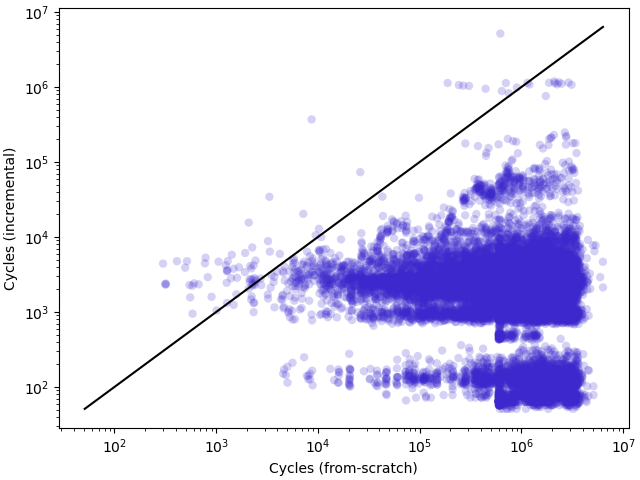
\includegraphics[width=\linewidth]{images/scatter-plot.png}
%DIFDELCMD < %%%
\DIFdelendFL \DIFaddbeginFL 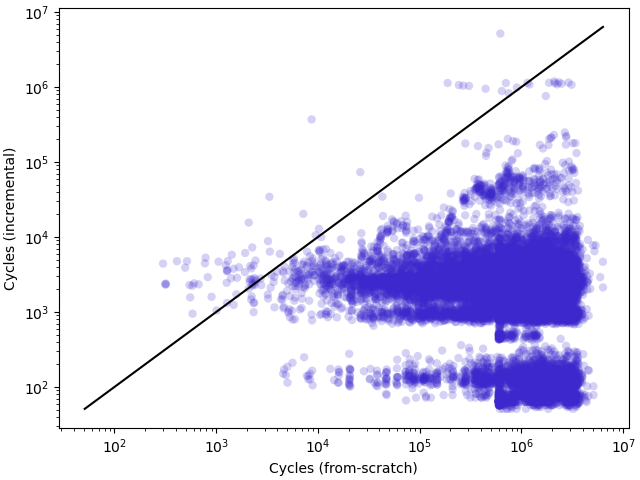
\includegraphics[width=0.75\linewidth]{images/scatter-plot.png}
\DIFaddendFL \caption{Incremental vs. from-scratch editing times}
\label{fig:scatter-plot}
\end{figure}

%\label{sec:Evaluation}
%\begin{figure}
%\begin{minipage}{.48\linewidth}
%    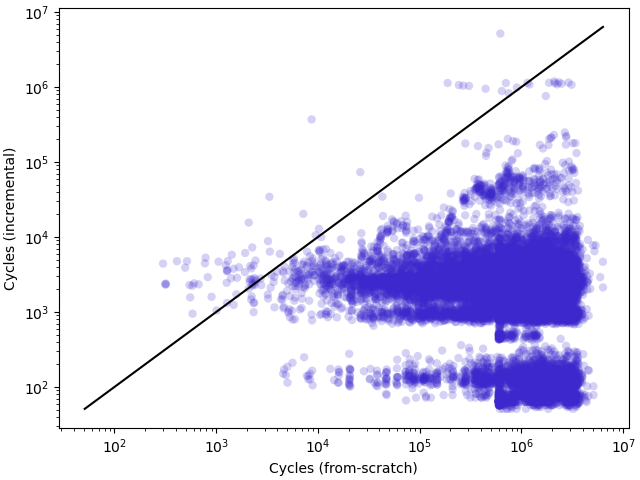
\includegraphics[width=\linewidth]{images/scatter-plot.png}
%    \caption{XXX}
%    \label{fig:scatter-plot}
%\end{minipage}
%\begin{minipage}{.48\linewidth}
%    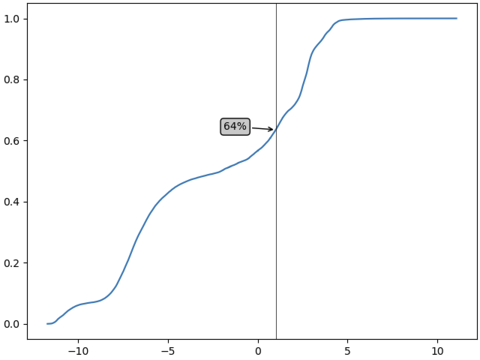
\includegraphics[width=\linewidth]{images/cdf.png}
%    \caption{YYY}
%    \label{fig:cdf}
%\end{minipage}
%\end{figure}

In this section we present our evaluation of the efficiency of Malcom relative to from-scratch type checking.  

\subsection{Benchmark}
We time Malcom on a synthesized edit trace constructed to test multiple aspects of Malcom. The first stage of the edit trace builds the program to a substantial size by constructing 100 nested copies of the merge sort algorithm. Each layer consists of a split function, a merge function, and a sort function. Each instance of the two helper functions, merge and split, is bound to a unique numbered identifier (\texttt{split\_n} and \texttt{merge\_n} for each layer \texttt{n}). Each sort function, on the other hand, is bound to the same identifier (\texttt{mergesort}). To capture long-distance binding patterns, each implementation of sort chooses which copy of split and which copy of merge to use uniformly at random from among those in scope. This  tests two aspects of Malcom's handling of bindings.

% The benchmark revolves around a `mergesort tower', a long chain of let-definitions, where the binding alternate between the options below:
% \begin{enumerate}
%     \item Binding a merge implementation to \texttt{merge\_n}, where \textsc{n} is the amount of previous merge definitions, to give each of them a unique name.
%     \item Binding a split implementation to \texttt{split\_n}.
%     \item Binding a mergesort implementation, which (at program construct time) randomly sample an available \texttt{merge\_n} and \textsc{split\_n} to depend on, to \texttt{mergesort}.
% \end{enumerate}
% Each of these options are defined and bounded to 100 times.

\begin{enumerate}
    \item \textbf{Shadowing}. Each \texttt{mergesort} shadows the one before it, testing Malcom's ability to find ancestor binders efficiently.
    \item \textbf{Name Reuse}. The definitions of \texttt{split\_n}, \texttt{merge\_n}, and \texttt{mergesort} each use common local variable names, such as \texttt{x}. Thus, those variable names are bound in multiple non-overlapping scopes, and Malcom must bind each occurrence to the correct binder.
    % \item \textbf{Irrelevant Names}. There are a multitude of different name, and name resolving should ignore irrelevant name, even though such names might change to shadow other variables in the future.
\end{enumerate}

The edit trace builds this tower by inserting constructors at leaves of the program sketch until complete. At each point in construction, the children of the current node in the sketch are constructed in a random order, and this proceeds recursively. This randomness ensures that different patterns of variable interactions are tested: for example, a variable binding might be inserted into an abstraction after its body has been constructed, capturing the free occurrences in the body.
% The program is built up randomly and recursively: to build a tree \textbf{X} at a Hole, the editor replace the hole with the root node of \textbf{X}, but with all children being empty Hole. It then randomly select a children which is not instantiated yet (so a hole), move down into it build it, and move up, repeating this process until all children had been instantiated. The randomness ensures different kinds of variable interactions are tested: for example, a variable binding might be inserted in the middle of the tree, thus shadowing the same binding from its ancestor, and being shadowed by the same binding from its descendents.

After the construction phase of the edit trace, random edits are applied throughout the program. Each of these edit sequences consists of moving to a uniformly random location in the program, applying a small change based on the node, and reverting the change. This is repeated 500 times. The changes include:
% After the program is built up, we apply random edits to the tree by selecting a random location, moving to the location, applying some small changes to the tree, and reverting our changes. The changes we apply includes:
\begin{enumerate}
    \item Deleting a leaf node and inserting another in its place.
    \item Replacing a binder with another.
    \item Wrapping a constructor around a subterm.
    \item Alternatively, for constructors with one child subexpression (for which unwrapping does not delete subexpressions), unwrapping the constructor.
\end{enumerate}
% \begin{enumerate}
%     \item Deleting an atom to insert an atom in its place, as the most basic 'incremental check'.
%     \item Deleting a binder and insert an existing binder to stress shadowing resolution.
%     \item Wrapping a Node with an unwrapping the node
%     \item Alternatively, if the Node have one children, so unwrapping will not lose information, unwrapping the node then wrapping it again to revert.
% \end{enumerate}
These edits test deletion, insertion, wrapping, and unwrapping, including updating types and binders. They also can introduce errors, demonstrating Malcom's incremental error marking ability.

\subsection{Results}
For each non-move edit, we measure the time it takes to perform the action and propagate updates until quiescent. Timing is done with \DIFdelbegin \DIFdel{the instruction rdtsc. The }\DIFdelend \DIFaddbegin \texttt{\DIFadd{rdtsc}}\DIFadd{. For a baseline, the }\DIFaddend same edit is performed on a bare syntax tree represented with \DIFaddbegin \DIFadd{a }\DIFaddend zipper data structure, and \DIFdelbegin \DIFdel{it }\DIFdelend is type checked from scratch according to the ordinary MALC marking procedure. The total time to edit and type check is compared between the incremental and from-scratch analyses. Note that action performance can be slower for Malcom than for the ordinary zipper representation, since Malcom computes changes to bindings at edit time. Figure \ref{fig:scatter-plot} show a scatter plot comparing these times (in cycles) for Malcom and the from-scratch analysis. Each data point is one non-move edit to the program. Points above the diagonal (shown in black)  are edits where the from-scratch analysis is faster than the incremental one, and below the diagonal is the converse. Almost all points are below the diagonal, meaning that incrementality provides a speedup in almost all cases. Many points are far below the diagonal, with incrementality providing one or more orders of magnitude of speedup. The data points are multi-modal, forming multiple horizontal bands. This indicates a fundamental algorithmic speedup: while the from-scratch analysis grows linearly in program size, empirically the incremental analysis shows hardly any growth. The horizontal bands are likely made up of different kinds of actions. The \DIFdelbegin \DIFdel{top most }\DIFdelend \DIFaddbegin \DIFadd{top-most }\DIFaddend band displays a slight positive trend, indicating cases where the incremental analysis does grow with the program size. This band likely contains edits that affect binding structure.

In total \DIFdelbegin \DIFdel{time }\DIFdelend across all of these edits, Malcom provides whopping \speedup speedup over from-scratch marking, demonstrating its substantial advantage over non-incremental analysis in providing continuous static feedback.

\section{Related Work}%
\label{sec:Related Work}

There is a large body of work on incremental computation~\cite{IC-Survey, IC-bib}, ranging from general frameworks such as Self-Adjusting Computation (SAC)~\cite{SAC}, Adaption~\cite{Adapton,AdaptonName}, and incremental Datalog engines ~\cite{SOUFFLE} to domain-specific approaches for lists~\cite{ICC}, databases~\cite{DDF}, and web browsers~\cite{tali-garseil}.

Order maintenance data structures, first introduced by \cite{OM}, are a common data structure across these approaches, appearing in various forms in both general frameworks like SAC~\cite{DBLP:conf/popl/AcarBH02} and domain-specific systems like web browser layout engines \cite{ST}.

When considering the specific problem tackled in this paper of incrementally maintaining type information in response to program edits, there have been prior efforts of both varieties as well. Our approach is a domain-specific approach targeted very specifically to bidirectional type checking with total error localization, building on recent advances, most notably the marked lambda calculus~\cite{DBLP:journals/pacmpl/ZhaoMDBPO24} which was described in \autoref{sec:Background}. Fundamental to our approach is the use of a structure editor calculus to represent changes. We are most directly inspired by Hazelnut~\cite{omar2017b}, which specified a bidirectionally typed structure editor calculus which was able to update type error marks locally at the cursor without needing recomputation. However, Hazelnut simply leaves edits that require distant changes to error marks undefined, making it impractical for real editing. Hazel, which was originally based on Hazelnut, now uses an approach based on the MLC, and we plan to integrate the approach from this paper into a future version of Hazel.

\DIFaddbegin \DIFadd{The small step approach to typing appears in prior work~\mbox{%DIFAUXCMD
\cite{DBLP:conf/rta/StumpKO11,DBLP:conf/esop/KuanMF07}}\hskip0pt%DIFAUXCMD
, in which typing is presented as a rewrite system and is analyzed using term-rewriting theory. The use of small steps to propagate types is similar to Incremental MALC, but without birdirectionality or total error localization. 
}

\DIFaddend \citet{DBLP:conf/kbse/SzaboEV16} and \citet{DBLP:journals/pacmpl/PacakES20} take a more general approach by translating typing rules to a Datalog program whose database of derived semantic facts can be incrementally updated as the facts that encode the \DIFdelbegin \DIFdel{source code of the }\DIFdelend program are added and removed. This generic approach is worthy of continued investigation, but is limited by the generality of the incremental update algorithm for the chosen implementation of Datalog. One particular challenge is accounting for binding structure in a way that leverages the incrementality when encoded in Datalog.  \citet{DBLP:journals/pacmpl/PacakES20} uses co-contextual typing~\cite{DBLP:conf/oopsla/ErdwegBKKM15}, in which binding information is propagated bottom up rather than top down, to overcome issues related to binding structure updates\DIFdelbegin \DIFdel{, though this requires maintaining additional co-contextual information and updating it on edits. 
We avoid this overhead.
}\DIFdelend \DIFaddbegin \DIFadd{. This approach, while fine grained enough to capture individual binding updates rather than whole-context changes, still requires traversing program spines when bindings are updated, potentially incurring linear time performance penalties. 
%DIF >  though this requires maintaining additional co-contextual information and updating it on edits. We avoid this overhead.
}\DIFaddend 

\citet{Demers1981IncrementalEF} discusses incremental evaluation of attribute grammars, proposing two different approaches. As with Datalog, it is possible to encode many type systems as attribute grammars, and indeed the setting in this paper is the Cornell Program Synthesizer~\cite{teitelbaum1981cornell}, one of the earliest structure editors and a pioneer in live semantic analysis. It may be that a generalized version of our approach would start to look like an incremental attribute grammar system, given analogies between synthesized and analyzed attributes and synthesized and analyzed types. We are not aware of a contemporary implementation of these ideas. 

Our approach in this paper is distinctive relative to these related approaches in that we start by approaching the problem from type-theoretic first principles, developing a formal semantics for type information propagation and proving its \DIFdelbegin \DIFdel{metatheory}\DIFdelend \DIFaddbegin \DIFadd{metatheoretic properties}\DIFaddend , then implementing it in a highly specialized manner targeted to the problem of incremental bidirectional typing. We believe it will be fruitful to continue to compare generic approaches to our more direct approach, and hope that the novel benchmark \DIFdelbegin \DIFdel{tasks developed here 
(which are generally more sophisticated than those used in prior work) }\DIFdelend \DIFaddbegin \DIFadd{task developed here 
%DIF >  (which are generally more sophisticated than those used in prior work) 
}\DIFaddend will be ported to other systems and lead to productive competition (and even more realistic or punishing benchmarks).

In addition to approaches leveraging incrementality derived from edits, there are a number of approaches that rely on memoization or caching to improve the performance of language implementations. This includes a large body of work on incremental build systems \cite{ALACARTE, SALSA}, which are in common use in industry. These systems generally operate at a coarse granularity, rebuilding entire compilation units (e.g. modules or packages) after changes. In contrast, our approach operates at a fine-grained level, on individual expressions. Consequently, our approach is more suitable for live programming environments where edits may occur many times per second.

This family of approaches also includes the system of \citet{DBLP:conf/sle/WachsmuthKVGV13}, which develops a name resolution and type analysis engine using dependent ``tasks'', which each capture one step of analysis. This approach is language-independent but again less fine-grained than our approach, operating primarily at the file level in the implemented system. Some of the approaches we take in Malcom, namely the use of a priority queue to maintain the update propagation frontier, are reminiscent of task analysis engine based approaches.

\citet{DBLP:conf/nfm/BusiDG19} \DIFdelbegin \DIFdel{formally }\DIFdelend specify memoized versions of standard typing rules and implement this system to achieve speedups on various small functional and imperative benchmarks\DIFaddbegin \DIFadd{, but their approach sometimes requires traversing large parts of the program when a variable binding changes}\DIFaddend .  

\DIFaddbegin \DIFadd{\mbox{%DIFAUXCMD
\citet{DBLP:conf/fpca/AdityaN91} }\hskip0pt%DIFAUXCMD
present a system that incrementalizes the Hindley-Milner type inference algorithm based on a call-graph analysis. It specifically incrementalizes the unification phase of type checking, operating at the granularity of changes to individual declarations. \mbox{%DIFAUXCMD
\citet{DBLP:conf/popl/Meertens83} }\hskip0pt%DIFAUXCMD
also presents an incremental system for unification-based type checking, which incrementally maintains the unification constraints generated by the program but does not incrementally solve them in general.  
}

\DIFadd{Incrementalization has also been applied to program analysis techniques, such as abstract interpretation~\mbox{%DIFAUXCMD
\cite{DBLP:conf/sigsoft/McPeakGR13,DBLP:conf/birthday/SeidlEV15,DBLP:conf/benevol/EsVR17,DBLP:conf/ecoop/Razafintsialonina25}}\hskip0pt%DIFAUXCMD
, symbolic execution~\mbox{%DIFAUXCMD
\cite{DBLP:conf/icse/YangKP04,DBLP:conf/issta/YangPK12,DBLP:journals/tosem/YangPRK14,DBLP:conf/icse/QiuYPK15}}\hskip0pt%DIFAUXCMD
, intermediate representation~\mbox{%DIFAUXCMD
\cite{DBLP:conf/indiaSE/GhimeKJC22}}\hskip0pt%DIFAUXCMD
, data flow for probabilistic programs~\mbox{%DIFAUXCMD
\cite{DBLP:conf/sas/ZhangSX17}}\hskip0pt%DIFAUXCMD
, and analysis via encoding as a constraint satisfaction problem~\mbox{%DIFAUXCMD
\cite{DBLP:conf/fase/MudduluruR14}}\hskip0pt%DIFAUXCMD
. Existing techniques for incremental abstract interpretation could be applied to type inference, but it is not clear how they would handle type error localization, fine grained incremental analysis, or concurrent editing and analysis. 
}

%DIF >  These techniques generally rely on dependency analysis and memoization.

%DIF >  ~\cite{DBLP:conf/scam/WautersPSR23} identifies edits of certain forms that have simple effects on the reanalysis (e.g. semantics preserving changes like consistently renaming a binder).

%DIF >  ~\cite{DBLP:conf/icse/LauterburgSMV08}






\DIFaddend % \subsection{Related Work Copied From Spineless Traversal}

% \paragraph{Incremental Computation}
% Incremental computation---%
%   speeding up computations by reusing previously-computed results---%
%   is a long-studied topic in computer science broadly~\cite{memo}
%   and programming language theory in particular;
%   \citet{IC-Survey} and \citet{IC-bib}
%   give thorough surveys of the field.
% The recent Self-Adjusting Computation (SAC)~\cite{SAC} framework
%   proposes incrementalizing arbitrary computations,
%   including a cost semantics~\cite{SACCost},
%   optimizations for data structure operations~\cite{SACTrace},
%   and opportunities for parallelization~\cite{PSAC}.
% The Adapton framework~\cite{Adapton}
%   aims at \emph{demand-driven} incremental computation,
%   and allows manually-specified annotations~\citet{AdaptonName}
%   for greater reuse.
% While this prior work focuses on general-purpose computations,
%   Spineless Traversal is focused on a particularly critical application of incremental computation: web browsers.
% This application-specific focus has precedent:
%   \citet{ICC} speed up memoization for functional programs over lists
%   using ``chunky decomposition'',
%   while differential dataflow databases~\cite{DDF}
%   incrementalize Relational Algebra computations
%   and have achieved some prominence in industry.
% \citet{TR1} is the earliest work
%   on incremental evaluation of attribute grammar,
%   motivated by syntax-directed editors;
% Later work~\cite{TR2} allows reference to non-neighbor attributes.
% However, these early papers require recomputation
%   immediately after every tree change,
%   whereas web browsers, our target application,
%   batch updates to perform incremental computation
%   only once per frame.
% The standard in web browsers is instead
%   the Double Dirty Bit algorithm,
%   implemented in all existing web rendering engines.
% \citet{tali-garseil} describes the Double Dirty Bit algorithm
%   in industry publication \texttt{web.dev},
%   and it also features in textbooks~\cite{wbe}.

% The formal methods community has put significant effort
%   into formalizing web page layout.
% \citet{meyerovich-1} proposed using attribute grammars,
%   similar to the DSL in Figure~\ref{fig:dsl},
%   for formalizing web-like layout rules.
% Later work~\cite{yufeng-1} proposes
%   synthesizing schedules from the attribute grammar rules,
%   including proposals~\cite{meyerovich-2,meyerovich-3}
%   to use parallel schedules to further improve layout performance.
% The Cassius project~\cite{cassius-1}
%   later formalized a significant fragment of CSS~2.1
%   using an attribute-grammar-like formalism.
% Our layout implementation is based on Cassius.
% Later work~\cite{cassius-2} also proposed
%   using the Cassius formalism to verify web page layouts,
%   including in a modular way~\cite{cassius-3}.
% However, none of these works investigated incremental layout.
% By contrast, the MEDEA project~\cite{yufeng-2}
%   proposed synthesizing incremental layout algorithms
%   by automatically synthesizing dirty bit propagation code.
% Our work extends MEDEA by exploring
%   optimized incremental traversal algorithms.

% \subsection{Related Work Copied from WITS Abstract}

% % This work follows the work on  in employing  The prior work on adaptive functional programming presents general translations to incremental programs, using order maintenance to prioritize the recomputation of intermediate values. On the other hand, the present work is specialized to bidirectional typing and uses order maintenance to maintain scoping data.

% Prior approaches to incremental typing utilize a task engine~\cite{DBLP:conf/sle/WachsmuthKVGV13},  or translate typing rules to a Datalog program that can be solved incrementally~\cite{DBLP:conf/kbse/SzaboEV16, DBLP:journals/pacmpl/PacakES20}. 

% This work follows the work in \cite{DBLP:conf/popl/AcarBH02}, which proposes a mechanism to make any purely-functional program adaptive using order maintenance for incremental computation. 

% \cite{DBLP:conf/stoc/DietzS87} describes the order maintenance data structure used in this paper to maintain scoping data.

% While our approach is specialized to the bidirectionally typed lambda calculus, more general prior approaches to incremental typing exist.


% \cite{DBLP:conf/nfm/BusiDG19} proposes a language-independent incrementalization using caching and memoization.

% \cite{DBLP:journals/pacmpl/PacakES20} and \cite{DBLP:conf/kbse/SzaboEV16} take the approach of compiling analyses to Datalog, for which incremental solvers already exist.

% \cite{DBLP:conf/oopsla/ErdwegBKKM15} uses the technique of co-contextual typing, propagating context \textit{requirements} up expression trees during type checking. The co-contextual typing rules naturally give rise to incrementality via memoization.

% \cite{}

%  The first involves two passes .... The second involves propagating changes.

% \cite{}




\section{Discussion and Conclusion}%
\label{sec:Discussion and Conclusion}
In this work we provide a formal system and efficient implementation for maintaining type information in a simple editor calculus. To serve as the base theory, we introduce the marked and annotated lambda calculus (MALC), a novel variant of the marked lambda calculus. 

Our incremental system is remarkably (pun intended) more efficient than from-scratch reanalysis. It contributes to the goal of live programming not just by being efficient, but by reducing the extent to which type checking blocks users from editing the program. 

% [alternative design: all local, no OM => less incremental, but less blocking]

\subsection{Future Work}
Incremental MALC and Malcom present several opportunities for extension and improvement. One notable limitation of our approach is that although update propagation is less blocking than a batch analysis, it is still possible for some individual update propagation steps to take a long time. In particular, those that involve traversing every occurrence of a variable bound by a particular binder block editing for a time proportional to the number of bound variables. Although this would not seem to be much of a problem in practice, future work may refine the approach and address this possibility. One potential strategy is for the binder to track which of its variables have been updated with new information and update the variables one at a time during update propagation.

While Incremental MALC expresses highly incremental expression-level analysis, it does not provide an incremental solution for type-level computations. Consistency checks, for example, must be rerun in their entirety when only part of the input changes. Although the size of types might often remain modest compared with the size of the program, it may be valuable to extend Incremental MALC with incremental type-level operations in future work. 

As described in \DIFdelbegin %DIFDELCMD < \autoref{subsec:Language Extensions}%%%
\DIFdelend \DIFaddbegin \autoref{subsec:generalization}\DIFaddend , Incremental MALC as presented in this work fits within a more general schema that can accommodate additional language features. We leave it to future work to define, prove correct, and explore the expressivity of such a schema. We also leave to future work the engineering, and perhaps additional research, necessary to scale these ideas up to real-world type systems. 

Incremental MALC supports liveness for only type-based editor services. To achieve large scale live programming requires incrementalized theories for other editor services, such as evaluation. There is much future work to be done in developing such theories. 
% - demand driven update prioritization


\newpage 
\section*{Data Availability Statement}

% https://github.com/hazelgrove/incremental-hazelnut/tree/submission-march
This paper is accompanied by two artifacts: an Agda mechanization of the definitions and proofs for Incremental MALC (presented in~\autoref{sec:Formalism}) and an OCaml implementation and interactive workbench of the Malcom incremental type system (described in~\autoref{sec:Implementation}). The Agda mechanization can be found at \url{https://github.com/hazelgrove/incremental-statics-agda} and the workbench can be found at \url{https://github.com/hazelgrove/incremental-hazelnut/tree/submission-march}.

%DIF <  \section*{Acknowledgments}
The authors would like to thank the anonymous referees at WITS 2025 and OOPSLA 2025 for their helpful feedback on this project. The authors would also like to thank Eric Zhao, Sebastian Erdweg, and Michael Arntzenius for their illuminating conversations related to this work, and thank Liam Mulcahy for his contributions to the accompanying workbench. We credit Kanat Tangwongsan, Yit Phang Khoo, and Matthew A. Hammer for their implementation of the order maintenance data structure. This work was partially funded by the National Science Foundation under Grant No. 2238744 and 2340192. Any opinions, findings, and conclusions or recommendations expressed in this material are those of the authors and do not necessarily reflect the views of the National Science Foundation.
\DIFaddbegin \section*{\DIFadd{Acknowledgments}}
\DIFadd{The authors would like to thank the anonymous referees at WITS 2025 and OOPSLA 2025 for their helpful feedback on this project. The authors would also like to thank Eric Zhao, Sebastian Erdweg, and Michael Arntzenius for their illuminating conversations related to this work, and thank Liam Mulcahy for his contributions to the accompanying workbench. We credit Kanat Tangwongsan, Yit Phang Khoo, and Matthew A. Hammer for their implementation of the order maintenance data structure. This work was partially funded by the National Science Foundation under Grant No. 2238744 and 2340192. Any opinions, findings, and conclusions or recommendations expressed in this material are those of the authors and do not necessarily reflect the views of the National Science Foundation.
}

\DIFaddend \bibliography{incremental-paper}

% \newpage 
% \appendix
% 
% \part{Appendix}

\section{Definitions for Incremental MALC}

The syntax of sorts relevant to MALC and Incremental MALC are given in~\autoref{fig:syntax}. The side conditions used for typing are defined in~\autoref{fig:side-conditions}. Note that these operations have been extended to accommodate optional types, as required in the action performance and update propagation step rules. The marking judgments for MALC are defined in~\autoref{fig:marking}. Simple and localized actions are defined in~\autoref{fig:actions}. The variable update judgment is defined in~\autoref{fig:variable-update}.~\autoref{fig:simple-action-perfomance} and~\autoref{fig:localized-action-perfomance} define the rules for simple action performance and localized action performance.~\autoref{fig:update} defines update propagation steps. Finally,~\autoref{fig:Well-Formedness} defines the well-formedness invariant. 

\begin{figure}
    \[\begin{array}{lcllll}
    \VV & \in & \VName &  & \\ 
    \BV & \in & \BName & \Coloneqq & \EHole \mid \VV \\ 
    \TV & \in & \TName & \Coloneqq & 
        \THole 
        \mid \TBase
        \mid \TArrow{\TV}{\TV} \\ 
    \DV & \in & \DName & \Coloneqq & 
        \DNone
        \mid \DSome{\tau}\\ 
    \BEV & \in & \BEName & \Coloneqq & 
        \BEHole
        \mid \BEConst
        \mid \BEVar{\VV}
        \mid \BELam{\BV}{\TV}{\BEV}
        \mid \BEAp{\BEV}{\BEV}
        \mid \BEAsc{\BEV}{\TV}\\
    \MV & \in & \MName & \Coloneqq & 
        \MGood
        \mid \MBad \\ 
    \MEUV & \in & \MEUName & \Coloneqq & \EUp{\MEMV~}{\DV}\\ 
    \MEMV & \in & \MEMName & \Coloneqq & 
        \EHole
        \mid \EConst
        \mid \EVar{\VV}{\MV}
        \mid \ELam{\BV}{\TV}{\MV}{\MV}{\MELV}
        \mid \EAp{\MELV}{\MV}{\MELV}
        \mid \EAsc{\MELV}{\TV}\\ 
    \MELV & \in & \MELName & \Coloneqq & \ELow{\DV}{\MV}{\MEUV}\\
    \MPV & \in & \MPName \subseteq \MELName & \Coloneqq & \ELow{\DNone}{\MGood}{\MEUV}\\ 
    \NVSymbol & \in & \NName & \Coloneqq & \raisebox{0.5pt}{\scalebox{1.3}{\NNewSymbolBlack}} \mid \NOldSymbol\\ 
    \EUV & \in & \EUName & \Coloneqq & \EUp{\EMV~}{\NDV}\\ 
    \EMV & \in & \EMName & \Coloneqq & 
        \EHole
        \mid \EConst
        \mid \EVar{\VV}{\MV}
        \mid \ELam{\BV}{\NTV}{\MV}{\MV}{\ELV}
        \mid \EAp{\ELV}{\MV}{\ELV}
        \mid \EAsc{\ELV}{\NTV}\\ 
    \ELV & \in & \ELName & \Coloneqq & \ELow{\NDV}{\MV}{\EUV}\\ 
    \PV & \in & \PName \subseteq \ELName & \Coloneqq & \ELow{\NV{\DNone}}{\MGood}{\EUV}\\ 
    \ctx & \in & \ctxName & \Coloneqq & \emptyset \mid \extendCtx{\ctx}{\VV}{\TV}\\
    \end{array}\]
    \caption{Syntax of MALC and Incremental MALC}
    \label{fig:syntax}
\end{figure}

\begin{figure}
    \centering

    \judgbox{\inCtx{\BV}{\TV}{\MV}{\ctx}}
    \vspace{-7pt}
    \[
    \inCtxHole\hspace{20pt}\inCtxEmpty\hspace{20pt}\inCtxFound\hspace{20pt}\inCtxSkip
    \]

    \judgbox{\matchedArrow{\DV}{\DV}{\DV}{\MV}}
    \vspace{-7pt}
    \[
    \matchedArrowNone\hspace{20pt}\matchedArrowHole\hspace{20pt}\matchedArrowArrow\hspace{20pt}\matchedArrowOther
    \]
    
    \judgbox{\consistent{\DV}{\DV}{\MV}}
    \vspace{-10pt}
    \[
    \consistentNoneL\hspace{20pt}\consistentNoneR\hspace{20pt}\consistentHoleL\hspace{20pt}\consistentHoleR
    \]
    \[
    \consistentArrow\hspace{20pt}\consistentOther
    \]
    \caption{Side Condition Judgments}
    \label{fig:side-conditions}
\end{figure}

\begin{figure}
    \centering

    \judgbox{\MarkSyn{\BEV}{\MEUV}}
    \[
    \MarkHole\hspace{20pt}\MarkConst\hspace{20pt}\MarkVar
    \]
    \[
    \MarkAsc\hspace{20pt}\MarkSynFun
    \]
    \[
    \MarkAp
    \]  

    \vspace{5pt}
    \judgbox{\MarkAna{\TV}{\BEV}{\MEUV}}
    \[
    \MarkSubsume
    \]
    \[
    \MarkAnaFun
    \]

    \vspace{5pt}
    \judgbox{\MarkProg{\BEV}{\MPV}}
    \[
    \MarkProgram
    \]
    \caption{Marking Judgments}
    \label{fig:marking}
\end{figure}

\begin{figure}
    \[\begin{array}{lclcll}
    \CV & \in & \CName & \Coloneqq & \One \mid\Two \\
        % \mid\Three \\
    \AV & \in & \AName & \Coloneqq & \InsertConst \mid \InsertVar{\VV} \mid \WrapFun \mid \WrapAp{\CV}\mid\WrapAsc\\
        &&&\mid &\Delete \mid \Unwrap{\CV}\mid \SetAnn{\TV} \mid \SetAsc{\TV}\\
        &&&\mid &\InsertBinder{\BV}\mid \DeleteBinder\\
    \overline{s} & \in & \mathsf{List[Sort]} & \Coloneqq & \nil \mid \cons{s}{\overline{s}}\\ 
    \LAV & \in & \LAName & \Coloneqq & \LA{\AV}{\overline{\CV}} 
    \end{array}\]
    \vspace{-10pt}
    \caption{Actions}
    \label{fig:actions}
\end{figure}

\begin{figure}
    \judgbox{\vsyn{\BV}{\MV}{\TV}{~\EUV}{\EUV}}
    \[
    \centering
    \VarUpdateHole\hspace{20pt}
    \VarUpdateVarEq\hspace{20pt}
    \VarUpdateVarNeq
    \]
     \[
    \centering
    \VarUpdateFunEq\hspace{20pt}
    \]
     \[
    \centering
    \VarUpdateFunNeq\hspace{20pt}
    \]
     \[
    \centering
    \VarUpdateAp
    \]
     \[
    \centering
    \VarUpdateAsc
    \]
     \[
    \centering
    \VarUpdateNone
    \]
    \caption{Variable Update Judgment}
    \label{fig:variable-update}
\end{figure}

\begin{figure}
    \judgbox{\ActUp{\AV}{\EUV}{\EUV}}

    \[
    \centering
    \ActInsertConst\hspace{30pt}
    \ActInsertVar\hspace{30pt}
    \ActDelete
    \]
    \[
    \centering
    \ActWrapFun\hspace{30pt}
    \ActWrapAsc
    \]
    \[
    \centering
    \ActWrapApOne
    \ActWrapApTwo
    \]
    \[
    \centering
    \ActUnwrapFun\hspace{20pt}
    \ActUnwrapAsc
    \]
    \[
    \centering
    \ActUnwrapApOne\hspace{20pt}
    \ActUnwrapApTwo
    \]
    \[
    \centering
    \ActSetAnn\hspace{10pt}
    \ActSetAsc
    \]
    \vspace{5pt}
    \[
    \centering
    \ActInsertBinder
    \]
    \[
    \centering
    \ActDeleteBinder
    \]

    \vspace{15pt}
    
    \judgbox{\ActLow{\AV}{\ELV}{\ELV}}
    % \hspace{80pt}\judgbox{\ActProg{\AV}{\PV}{\PV}}
    \[
    \centering
    \ActAna
    % \hspace{80pt}\ActProgram
    \]
    \caption{Simple Action Performance}
    \label{fig:simple-action-perfomance}
\end{figure}

\begin{figure}
    \judgbox{\ActMid{\LAV}{\EMV}{\EMV}}
    \[
    \centering
    \ActFunRec\hspace{20pt}
    \ActAscRec
    \]
    \[
    \centering
    \ActApRecOne\hspace{20pt}
    \ActApRecTwo
    \]
    \judgbox{\ActLow{\LAV}{\EUV}{\EUV}}\hspace{5pt}
    \judgbox{\ActLow{\LAV}{\ELV}{\ELV}}\hspace{5pt}
    \judgbox{\ActProg{\LAV}{\PV}{\PV}}
    \[
    \centering
    \ActSynRec\hspace{20pt}
    \ActAnaRec\hspace{20pt}
    \ActAnaLocal\hspace{20pt}
    \ActProgram
    \]
    \caption{Localized Action Performance}
    \label{fig:localized-action-perfomance}
\end{figure}


\begin{figure}
    \judgbox{\funsyn{\DV}{\TV}{\DV}=\DV}
    \[\begin{array}{lcl}
        \funsyn{\DSome{\TV_1}}{\TV_2}{\DV} &=& \DNone\\
        \funsyn{\DNone}{\TV_2}{\DNone} &=& \DNone\\
        \funsyn{\DNone}{\TV_1}{\TV_2} &=& \TArrow{\TV_1}{\TV_2}
    \end{array}\]
    \judgbox{\StepLow{\ELV}{\ELV}}
    \[
    \centering
    \StepSyn \hspace{20pt}
    \StepAna
    \]
    \[
    \centering
    \]
    \[
    \centering
    \StepAnnFun \hspace{20pt}
    \StepSynFun
    \]
    \[
    \centering
    \StepAnaFun~+~\text{cong. rules}
    \]
    
    \judgbox{\StepUp{\EUV}{\EUV}}
    \[
    \centering
    \StepAp\hspace{20pt}
    \StepAsc~+~\text{cong. rules}
    \]
    
    \judgbox{\StepProg{\PV}{\PV}}
    \[
    \centering
    \InsideStep\hspace{20pt}\TopStep
    \]
    
    \caption{Update Propagation Steps}
    \label{fig:update}
\end{figure}


% \section{Well-Formedness}
% \label{subsec:Well-Formedness}
% Stating and proving the correctness properties of the calculus rely on the notion of a well-formed program. This is the invariant on incremental programs that is preserved by all actions and update propagation steps and ensures the equivalence of the incremental analysis and the from-scratch analysis. The definition of this predicate, denoted $\WFP{\PV}$, is in \autoref{fig:Well-Formedness}. 

\begin{figure}
    \judgbox{\matchedArrow{\NDV}{\NDV}{\NDV}{\NV{\MV}}}\hspace{10pt}
    \judgbox{\consistent{\NDV}{\NDV}{\NV{\MV}}}
    \[
    \matchedArrowDirty\hspace{30pt}\consistentDirty
    \]
    
    \judgbox{\WFU{\EUV}}\hspace{10pt}\judgbox{\WFL{\ELV}}
    \[
    \WFHole\hspace{20pt}\WFConst\hspace{20pt}\WFVar\hspace{20pt}\WFAsc
    \]
    \[
    \WFAp
    \]
    \[
    \WFSubsume
    \]
    \[
    \WFFun
    \]
    
    \judgbox{\ncon{\NV{a}}{a}}\hspace{85pt}
    \judgbox{\WFP{\PV}}
    \[
    \NconNew\hspace{20pt}\NconOld\hspace{60pt}
    \WFProgram
    \]
    \caption{The Well-Formedness Invariant}
    \label{fig:Well-Formedness}
\end{figure}

\paragraph{Well-Formedness} Well-formedness is defined in a syntax-directed way on all analytic expressions, with the \rulename{WFSyn} rule and the $\WFU{\EUV}$ judgment serving as a convenience for factoring the consistency check out of $\WFL{\ELV}$ for subsumable forms. The predicate utilizes the ``directed consistency'' relation, $\ncon{\NV{a}}{a}$. This relation holds when either the first argument is dirty or the arguments carry the same value. Programs are well-formed when this relation holds at every step of the bidirectional information flow. For example, in the rule \rulename{WFAp}, the analyzed type $\NDV_1$ is matched as an arrow type, resulting in a domain type, codomain type, and mark. This information, which was derived from the upstream type, are checked with the directed consistency relation against the downstream information found in the program. This check ensures that the information in the incremental program is locally consistent, except at the frontier of update propagation. Variants of the side condition judgments are introduced which operate on dirtied types, which produce dirty outputs if any inputs are dirty. Actions maintain this invariant by dirtying any information that may be newly inconsistent with its surroundings, and updates maintain the invariant by progressing the frontier according to the correct typing rules.

\FloatBarrier

\section{Polymorphic Incremental MALC}
\label{subsec:appendix-polymorphism}

% Below are the syntax, marking, action performance, update step propagation, and well-formedness rules for the polymorphic extension of Incremental MALC are. Only the rules for the new syntactic forms are included in the action performance, update step propagation, and well-formedness figures, with the other rules 

\begin{figure}[ht]
    \[\begin{array}{lcllll}
    \VV & \in & \VName &  & \\  
    \TVV & \in & \TVName &  & \\ 
    \BV & \in & \BName & \Coloneqq & \EHole \mid \VV \\
    \TBV & \in & \TBName & \Coloneqq & \EHole \mid \TVV \\
    \BTV & \in & \BTName & \Coloneqq & 
        \THole 
        \mid \TBase
        \mid \TArrow{\BTV}{\BTV} 
        \mid \TVar{\TVV} 
        \mid \TForall{\TBV}{\BTV}\\ 
    % \DV & \in & \DName & \Coloneqq & 
    %     \DNone
    %     \mid \DSome{\tau}\\ 
    \BEV & \in & \BEName & \Coloneqq & 
        \BEHole
        \mid \BEConst
        \mid \BEVar{\VV}
        \mid \BELam{\BV}{\TV}{\BEV}
        \mid \BEAp{\BEV}{\BEV}
        \mid \BEAsc{\BEV}{\TV}\\
        &&& \mid & \BETLam{\TBV}{\BEV} 
        \mid \BETAp{\BEV}{\TV}\\
    \MV & \in & \MName & \Coloneqq & 
        \MGood
        \mid \MBad \\ 
    \MTV & \in & \MTName & \Coloneqq & 
        \THole 
        \mid \TBase
        \mid \TArrow{\MTV}{\MTV} 
        \mid \MTVar{\TVV}{\MV} 
        \mid \TForall{\TBV}{\MTV} \\ 
    \MDV & \in & \MDName & \Coloneqq & 
        \DNone
        \mid \DSome{\MTV}\\ 
    \MEUV & \in & \MEUName & \Coloneqq & \EUp{\MEMV~}{\MDV}\\ 
    \MEMV & \in & \MEMName & \Coloneqq & 
        \EHole
        \mid \EConst
        \mid \EVar{\VV}{\MV}
        \mid \ELam{\BV}{\MTV}{\MV}{\MV}{\MELV}
        \mid \EAp{\MELV}{\MV}{\MELV}
        \mid \EAsc{\MELV}{\MTV}\\
        &&& \mid & \ETLam{\TBV}{\MV}{\MEMV} 
        \mid \ETAp{\MEMV}{\MV}{\NV{\MTV}}\\ 
    \MELV & \in & \MELName & \Coloneqq & \ELow{\MDV}{\MV}{\MEUV}\\
    \MPV & \in & \MPName \subseteq \MELName & \Coloneqq & \ELow{\DNone}{\MGood}{\MEUV}\\ 
    \NVSymbol & \in & \NName & \Coloneqq & \raisebox{0.5pt}{\scalebox{1.3}{\NNewSymbolBlack}} \mid \NOldSymbol\\ 
    \EUV & \in & \EUName & \Coloneqq & \EUp{\EMV~}{\NMDV}\\ 
    \EMV & \in & \EMName & \Coloneqq & 
        \EHole
        \mid \EConst
        \mid \EVar{\VV}{\MV}
        \mid \ELam{\BV}{\NMTV}{\MV}{\MV}{\ELV}
        \mid \EAp{\ELV}{\MV}{\ELV}
        \mid \EAsc{\ELV}{\NMTV}\\
        &&& \mid & \ETLam{\TBV}{\MV}{\EMV} 
        \mid \ETAp{\EMV}{\MV}{\NMTV}\\ 
    \ELV & \in & \ELName & \Coloneqq & \ELow{\NMDV}{\MV}{\EUV}\\ 
    \PV & \in & \PName \subseteq \ELName & \Coloneqq & \ELow{\NV{\DNone}}{\MGood}{\EUV}\\ 
    \ctx & \in & \ctxName & \Coloneqq & 
        \emptyset 
        \mid \extendCtx{\ctx}{\VV}{\MTV}
        \mid \tExtendCtx{\ctx}{\TVV}\\
    \end{array}\]
    \vspace{-10pt}
    \caption{Syntax of Polymorphic Incremental MALC}
    \label{fig:appendix-polymorphism-syntax}
\end{figure}

\begin{figure}[h]
    \[\begin{array}{lclcll}
    \CV & \in & \CName & \Coloneqq & \One \mid\Two \\
        % \mid\Three \\
    \AV & \in & \AName & \Coloneqq & \InsertConst \mid \InsertVar{\VV} \mid \WrapFun \mid \WrapAp{\CV}\mid\WrapAsc\\
        &&&\mid &\Delete \mid \Unwrap{\CV}\mid \SetAnn{\TV} \mid \SetAsc{\TV}\\
        &&&\mid &\InsertBinder{\BV}\mid \DeleteBinder\\
        &&&\mid &\WrapTFun \mid \WrapTAp \mid \SetTArg{\TV}\\
    \overline{s} & \in & \mathsf{List[Sort]} & \Coloneqq & \nil \mid \cons{s}{\overline{s}}\\ 
    \LAV & \in & \LAName & \Coloneqq & \LA{\AV}{\overline{\CV}} 
    \end{array}\]
    \vspace{-10pt}
    \caption{Polymorphism Actions}
    \label{fig:appendix-polymorphism-actions}
\end{figure}

\begin{figure}
    \centering

    \judgbox{\MarkTyp{\BTV}{\MTV}}
    \[
    \MarkTHole \hspace{20pt} \MarkTBase \hspace{20pt} \MarkTArrow
    \]
    \[
    \MarkTVar \hspace{20pt} \MarkForall
    \]

    \judgbox{\MarkSyn{\BEV}{\MEUV}}
    \[
    \MarkHole\hspace{20pt}\MarkConst\hspace{20pt}\PolyMarkVar
    \]
    \[
    \PolyMarkAsc\hspace{20pt}\PolyMarkSynFun
    \]
    \[
    \PolyMarkAp
    \]
    \[
    \MarkSynTFun \hspace{20pt} \MarkTAp
    \]

    \vspace{5pt}
    \judgbox{\MarkAna{\MTV}{\BEV}{\MEUV}}
    \[
    \PolyMarkSubsume
    \]
    \[
    \PolyMarkAnaFun
    \]
    \[
    \MarkAnaTFun
    \]

    % \vspace{5pt}
    % \judgbox{\MarkProg{\BEV}{\MPV}}
    % \[
    % \MarkProgram
    % \]
    
    \vspace{-10pt}
    \caption{Polymorphism Marking Judgments}
    \label{fig:appendix-polymorphism-marking}
\end{figure}

% \begin{figure}
%     \judgbox{\vsyn{\BV}{\MV}{\TV}{~\EUV}{\EUV}}
%     \[
%     \centering
%     \VarUpdateHole\hspace{20pt}
%     \VarUpdateVarEq\hspace{20pt}
%     \VarUpdateVarNeq
%     \]
%      \[
%     \centering
%     \VarUpdateFunEq\hspace{20pt}
%     \]
%      \[
%     \centering
%     \VarUpdateFunNeq\hspace{20pt}
%     \]
%      \[
%     \centering
%     \VarUpdateAp
%     \]
%      \[
%     \centering
%     \VarUpdateAsc
%     \]
%      \[
%     \centering
%     \VarUpdateNone
%     \]
%     \caption{Polymorphism variable update judgments}
%     \label{fig:polymorphism-variable-update}
% \end{figure}


\begin{figure}
    \centering

    \judgbox{\ActUp{\AV}{\BTV}{\MTV}}
    \[
    ...\hspace{20pt} \ActWrapTFun \hspace{20pt} \ActSetTArg  
    % \ActWrapTAp
    \]
    % \[
    % \ActSetTArg 
    % \]
    \[
    \ActUnwrapTFun \hspace{20pt} \ActUnwrapTAp
    \]
    % \[
    % \ActInsertTBinder
    % \]
    % \[
    % \ActDeleteTBinder
    % \]
%     \vspace{-10pt}
%     \caption{Polymorphism Simple Action Performance}
%     \label{fig:appendix-polymorphism-actions}
% \end{figure}

% \begin{figure}
    \centering

    \judgbox{\StepLow{\ELV}{\ELV}}
    \[
    ...\hspace{20pt} \StepAnaTFun \hspace{20pt} \StepSynTFun
    \]
    \judgbox{\StepUp{\EUV}{\EUV}}
    \[
    ...\hspace{20pt} \StepTApFun \hspace{20pt} \StepTApArg
    \]
%     \vspace{-10pt}
%     \caption{Polymorphism Update Propagation Steps}
%     \label{fig:appendix-polymorphism-updates}
% \end{figure}

% \begin{figure}
    \judgbox{\WFU{\EUV}}
    \[
    ...\hspace{20pt} \WFTAp
    \]
    \judgbox{\WFL{\ELV}}
    \[
    \WFTFun
    \]
    \caption{Polymorphim Simple Action Performance, Update Propagation, and Well-Formedness Invariant}
    \label{fig:polymorphism-Well-Formedness}
\end{figure}

\FloatBarrier

\section{Properties of Incremental MALC}
\label{subsec:Proofs}

% \begin{figure}
%     \centering 
%     \caption{Interleaved action and update propagation}
%     \label{fig:actstep}
% \end{figure}

% \begin{theorem}[Action Completeness]
%     For any bare expressions $\BEV_1$ and $\BEV_2$, there exists a sequence of localized actions $\overline{\LAV}$ such that \ActProg{\overline{\LAV}}{\BEV_1}{\BEV_2} (where \ActProg{\overline{\LAV}}{\BEV_1}{\BEV_2} denotes iterated action performance). 
% \end{theorem}

This section describes the formal properties proven for Incremental MALC. The full proofs are available in the accompanying Agda mechanization. 

We begin with validity, which is expressed in terms of the relation $\ActStep{\overline{\LAV}}{\PV}{\PV}$, modeling interleaved action performance and update propagation, as well as the well-markedness condition on programs. 

\[
\ActStepAct\hspace{20pt}
\ActStepStep\hspace{20pt}
\ActStepDone
\]


\begin{definition}[Well-Markedness]
    A program $\PV$ is \textit{well-marked} if $\MarkProg{\erase{\PV}}{\MPV}$, where $\MPV$ is equal to $\PV$ up to dirtiness of types. 
\end{definition}

\begin{theorem}[Validity]
\label{theorem:Validity}
    If program $\PV$ is well-formed and $\ActStep{\overline{\LAV}}{\PV}{\PV'}$, then $\PV'$ is well-marked. 
\end{theorem}

Validity guarantees that the result of the incremental analysis agrees with the from-scratch static analysis. The following lemmas and definition are used in the proof:

\begin{lemma}[Action Preservation]
\label{lemma:Action Preservation}
    If $\PV$ is well-formed and $\ActProg{\LAV}{\PV}{\PV'}$, then $\PV'$ is well-formed. 
\end{lemma}

\begin{lemma}[Update Step Preservation]
\label{lemma:Update Step Preservation}
    If $\PV$ is well-formed and $\StepProg{\PV}{\PV'}$, then $\PV'$ is well-formed. 
\end{lemma}

\begin{definition}[Quiescent]
    An incremental program $\PV$ is \textit{quiescent} if it contains no dirty types. 
\end{definition}

\begin{lemma}[Progress]
\label{lemma:Progress}
    If $\PV$ is well-formed, then it can take an update step if and only if it is not quiescent. 
\end{lemma}

\begin{lemma}[Quiescent Validity]
\label{lemma:Quiescent Validity}
    If $\PV$ is well-formed and quiescent, then it is well-marked.  
\end{lemma}

These can be composed in a straightforward way to prove validity. Since $\PV$ is well-formed and $\ActStep{\overline{\LAV}}{\PV}{\PV'}$, then by~\autoref{lemma:Action Preservation} and~\autoref{lemma:Update Step Preservation} (action preservation and update step preservation) $\PV'$ is also well-formed. No steps are possible from $\PV'$, \autoref{lemma:Progress} (progress) ensures that it is quiescent. \autoref{lemma:Quiescent Validity} (quiescent validity) can then be applied to obtain the guarantee of well-markedness. 

\begin{theorem}[Convergence]
    If program $\PV$ is well-formed, $\ActStep{\overline{\LAV}}{\PV}{\PV_1}$, and $\ActStep{\overline{\LAV}}{\PV}{\PV_2}$, then $\PV_1=\PV_2$. 
\end{theorem}

Convergence is proven with the help of the following lemmas:

\begin{lemma}[Action Erasure]
\label{lemma:Action Erasure}
    If \ActProg{\LAV}{\PV}{\PV'}, then
    \ActProg{\LAV}{\erase{\PV}}{\erase{\PV'}}.
\end{lemma}

\begin{lemma}[Update Step Erasure]
\label{lemma:Update Step Erasure}
    If \StepProg{\PV}{\PV'}, then
    ${\erase{\PV}}={\erase{\PV'}}$.
\end{lemma}

\begin{lemma}[Action Unicity]
\label{lemma:Action Unicity}
    If \ActProg{\LAV}{\BEV}{\BEV_1} and \ActProg{\LAV}{\BEV}{\BEV_2}, then $\BEV_1=\BEV_2$.
\end{lemma}

\begin{lemma}[Marking Unicity]
\label{lemma:Marking Unicity}
    If $\MarkProg{\BEV}{\PV_1}$ and $\MarkProg{\BEV}{\PV_2}$, then $\PV_1=\PV_2$.  
\end{lemma}

Assuming $\PV$ is well-formed, $\ActStep{\overline{\LAV}}{\PV}{\PV_1}$, and $\ActStep{\overline{\LAV}}{\PV}{\PV_2}$, then ~\autoref{lemma:Action Erasure} and~\autoref{lemma:Update Step Erasure} (action erasure and update step erasure) imply that \ActProg{\overline{\LAV}}{\erase{\PV}}{\erase{\PV_1}} and \ActProg{\overline{\LAV}}{\erase{\PV}}{\erase{\PV_2}}. By \autoref{lemma:Action Unicity} (action unicity), $\erase{\PV_1}=\erase{\PV_2}$. By~\autoref{theorem:Validity} (validity), $\PV_1$ and $\PV_2$ are well-marked, meaning that $\MarkProg{\erase{\PV_1}}{\PV_1}$ and $\MarkProg{\erase{\PV_2}}{\PV_2}$. Using \autoref{lemma:Marking Unicity} (marking unicity) and the fact that $\erase{\PV_1}=\erase{\PV_2}$, we obtain $\PV_1=\PV_2$.   

\begin{theorem}[Termination]
    There is no infinite sequence $\{\PV_n\}_{n= 0}^\infty$ such that $\forall n$. $\StepProg{\PV_n}{\PV_{n+1}}$. 
\end{theorem}

Termination is proven by defining a well-founded ordering $<_P$ on programs such that if $\StepProg{\PV}{\PV'}$, then $\PV' <_P \PV$. Informally, $\PV' <_P \PV$ if either $\PV'$ has strictly fewer dirty types in the surface syntax (that is, on function annotations or type ascriptions), or $\PV'$ and $\PV$ have an equal number of such dirty types, but the update propagation frontier of $\PV'$ is further downstream than that of $\PV$ in the bidirectional flow. The syntax for incremental programs was designed to have the property that the left-to-right order in which annotations appear corresponds to the downstream order of information flow. All update rules except for those dealing with types in the surface syntax only dirty types to the right of the type they clean.


\end{document}